%%%%%%%%%%%%%%%%%%%%%%%%%%%%%%%%%%%%%%%%%
% Masters/Doctoral Thesis 
% LaTeX Template
% Version 2.4 (22/11/16)
%
% This template has been downloaded from:
% http://www.LaTeXTemplates.com
%
% Version 2.x major modifications by:
% Vel (vel@latextemplates.com)
%
% This template is based on a template by:
% Steve Gunn (http://users.ecs.soton.ac.uk/srg/softwaretools/document/templates/)
% Sunil Patel (http://www.sunilpatel.co.uk/thesis-template/)
%
% Template license:
% CC BY-NC-SA 3.0 (http://creativecommons.org/licenses/by-nc-sa/3.0/)
%
%%%%%%%%%%%%%%%%%%%%%%%%%%%%%%%%%%%%%%%%%

%----------------------------------------------------------------------------------------
%	PACKAGES AND OTHER DOCUMENT CONFIGURATIONS
%----------------------------------------------------------------------------------------

\documentclass[
11pt, % The default document font size, options: 10pt, 11pt, 12pt
%oneside, % Two side (alternating margins) for binding by default, uncomment to switch to one side
english, % ngerman for German
singlespacing, % Single line spacing, alternatives: onehalfspacing or doublespacing
%draft, % Uncomment to enable draft mode (no pictures, no links, overfull hboxes indicated)
%nolistspacing, % If the document is onehalfspacing or doublespacing, uncomment this to set spacing in lists to single
%liststotoc, % Uncomment to add the list of figures/tables/etc to the table of contents
%toctotoc, % Uncomment to add the main table of contents to the table of contents
%parskip, % Uncomment to add space between paragraphs
%nohyperref, % Uncomment to not load the hyperref package
headsepline, % Uncomment to get a line under the header
%chapterinoneline, % Uncomment to place the chapter title next to the number on one line
%consistentlayout, % Uncomment to change the layout of the declaration, abstract and acknowledgements pages to match the default layout
]{MastersDoctoralThesis} % The class file specifying the document structure

\usepackage[utf8]{inputenc} % Required for inputting international characters
\usepackage[T1]{fontenc} % Output font encoding for international characters

\usepackage{palatino} % Use the Palatino font by default

\usepackage[backend=bibtex,style=numeric,firstinits=true,natbib=true,sorting=none]{biblatex} % Use authoryear citation style for "Author, year" citation style

\addbibresource{references.bib} % The filename of the bibliography

%\usepackage{refcheck} % checks for correct reference usage and produces warnings; enable \nocite command

\usepackage[autostyle=true]{csquotes} % Required to generate language-dependent quotes in the bibliography

\usepackage{float} % In order to use the [H] option for figure alignment

\usepackage{fancyvrb} % keep tabs in verbatim sections, see: https://tex.stackexchange.com/questions/231083/how-to-stop-verbatim-from-converting-tabs-to-spaces

\usepackage{listings} % enable to reference source code, see: https://tex.stackexchange.com/questions/74155/how-to-treat-verbatim-as-a-block-that-can-be-referenced-just-like-a-figure

\usepackage{amssymb} % The amssymb package provides various useful mathematical symbols

\usepackage{mathtools} % math tools (ceiling signs, see: http://tex.stackexchange.com/questions/42271/floor-and-ceiling-functions)
\DeclarePairedDelimiter{\ceil}{\lceil}{\rceil}

% following packages allows to write algorithms as pseudocode
\usepackage{amsmath}
\usepackage{algorithmicx}
\usepackage{algorithm}
\usepackage{algpseudocode}
\algnewcommand\algorithmicinput{\textbf{INPUT:}}
\algnewcommand\INPUT{\item[\algorithmicinput]}
\algnewcommand\algorithmicoutput{\textbf{OUTPUT:}}
\algnewcommand\OUTPUT{\item[\algorithmicoutput]}

\usepackage{caption}
\captionsetup{width=0.8\textwidth} % global width of captions in figures, tables, etc. https://tex.stackexchange.com/questions/110393/too-wide-figure-caption

%----------------------------------------------------------------------------------------
%	COMMAND DEFINITIONS
%----------------------------------------------------------------------------------------

\definecolor{todoColor}{rgb}{1,0.55,0.2}
\newcommand{\todo}[1]{\textit{\color{todoColor}#1}}

% define commands to keep the formatting separated from the content 
\newcommand{\keyword}[1]{\textbf{#1}}
%\newcommand{\tabhead}[1]{\textbf{#1}}
\newcommand{\code}[1]{\texttt{#1}}
\newcommand{\file}[1]{\texttt{\bfseries#1}}
\newcommand{\option}[1]{\texttt{\itshape#1}}
\newcommand{\tabhead}[1]{\textbf{#1}}
\newcommand*\diff{\mathop{}\!\mathrm{d}} % dx
\newcommand*\Diff[1]{\mathop{}\!\mathrm{d^#1}} % d^2x
\newcommand{\mtrx}[1]{\mathbf{#1}}

%----------------------------------------------------------------------------------------
%	MARGIN SETTINGS
%----------------------------------------------------------------------------------------

\geometry{
	paper=a4paper, % Change to letterpaper for US letter
	inner=2.5cm, % Inner margin
	outer=3.8cm, % Outer margin
	bindingoffset=.5cm, % Binding offset
	top=1.5cm, % Top margin
	bottom=1.5cm, % Bottom margin
	%showframe, % Uncomment to show how the type block is set on the page
}

%----------------------------------------------------------------------------------------
%	THESIS INFORMATION
%----------------------------------------------------------------------------------------
\title{Doctoral Thesis}
\thesistitle[0, 0]{Multimesh Methods for Data Visualization and Finite Element Analysis} % Your thesis title, this is used in the title and abstract, print it elsewhere with \ttitle
\thesistitlecs{V\'ices\'i\v{t}ov\'e metody pro vizualizaci dat a v\'ypo\v{c}ty MKP} % Your thesis title in Czech, this is used in the title and abstract, print it elsewhere with \ttitlecs
\supervisor{prof. Ing. Jaroslav Kruis, Ph.D.} % Your supervisor's name, this is used in the title page, print it elsewhere with \supname
\examiner{} % Your examiner's name, this is not currently used anywhere in the template, print it elsewhere with \examname
\degree{Doctor of Philosophy} % Your degree name, this is used in the title page and abstract, print it elsewhere with \degreename
\author{Ing. \v{S}t\v{e}p\'{a}n Bene\v{s}} % Your name, this is used in the title page, print it elsewhere with \authorname
\authornodegree{\v{S}t\v{e}p\'{a}n Bene\v{s}} % Your name without degrees, this is used in the abstract and declaration page, print it elsewhere with \authornamenodegree
\addresses{Th\'akurova 7, 166 29 Praha 6} % Your address, this is not currently used anywhere in the template, print it elsewhere with \addressname

\subject{Engineering software} % Your subject area, this is not currently used anywhere in the template, print it elsewhere with \subjectname
\keywords{Finite Element Method (FEM), Finite Element Analysis (FEA), Post-processing, Data visualization, Data compression, Data management, Singular Value Decomposition (SVD)} % Keywords for your thesis, this is not currently used anywhere in the template, print it elsewhere with \keywordnames
\keywordscs{Metoda kone\v{c}n\'ych prvk\r{u} (MKP), Kone\v{c}n\v{e} prvkov\'a anal\'yza, Vizualizace dat, Komprese dat, Spr\'ava dat, Singul\'arn\'i rozklad (SVD)} % Keywords for your thesis, this is not currently used anywhere in the template, print it elsewhere with \keywordnames
\university{\href{http://www.cvut.cz}{Czech Technical University in Prague}} % Your university's name and URL, this is used in the title page and abstract, print it elsewhere with \univname
\department{\href{http://mech.fsv.cvut.cz}{Department of Mechanics}} % Your department's name and URL, this is used in the title page and abstract, print it elsewhere with \deptname
\faculty{\href{http://www.fsv.cvut.cz}{Faculty of Civil Engineering}} % Your faculty's name and URL, this is used in the title page and abstract, print it elsewhere with \facname

\AtBeginDocument{
\hypersetup{pdftitle=\ttitle} % Set the PDF's title to your title
\hypersetup{pdfauthor=\authorname} % Set the PDF's author to your name
\hypersetup{pdfkeywords=\keywordnames} % Set the PDF's keywords to your keywords
}

%----------------------------------------------------------------------------------------
%	SOURCE CODE STYLE
%----------------------------------------------------------------------------------------

\usepackage{inconsolata}

\definecolor{keywordsColor}{rgb}{0,0,1}
\definecolor{commentsColor}{rgb}{0,0.5,0}
\definecolor{stringsColor}{rgb}{0.64,0.08,0.08}
\definecolor{xmlcommentsColor}{rgb}{0.5,0.5,0.5}
\definecolor{typesColor}{rgb}{0.17,0.57,0.68}
\definecolor{numbersColor}{rgb}{0.25,0.6,0.83}

\usepackage{listings}
\lstset{language=[Sharp]C,
%captionpos=b,
%numbers=left, %Nummerierung
%numberstyle=\tiny, % kleine Zeilennummern
frame=lines, % Oberhalb und unterhalb des Listings ist eine Linie
showspaces=false,
showtabs=false,
breaklines=true,
showstringspaces=false,
breakatwhitespace=true,
escapeinside={(*@}{@*)},
commentstyle=\color{commentsColor},
morekeywords={partial, var, value, get, set},
keywordstyle=\color{keywordsColor},
stringstyle=\color{stringsColor},
basicstyle=\ttfamily\tiny,
}

\newcommand\JSONnumbervaluestyle{\color{numbersColor}}
\newcommand\JSONstringvaluestyle{\color{stringsColor}}

% switch used as state variable
\newif\ifcolonfoundonthisline

\makeatletter

\lstdefinestyle{json}
{
  showstringspaces    = false,
  keywords            = {false,true},
  alsoletter          = 0123456789.,
  morestring          = [s]{"}{"},
  stringstyle         = \ifcolonfoundonthisline\JSONstringvaluestyle\fi,
  MoreSelectCharTable =%
    \lst@DefSaveDef{`:}\colon@json{\processColon@json},
  basicstyle          = \ttfamily\tiny,
  keywordstyle        = \ttfamily\bfseries,
}

% flip the switch if a colon is found in Pmode
\newcommand\processColon@json{%
  \colon@json%
  \ifnum\lst@mode=\lst@Pmode%
    \global\colonfoundonthislinetrue%
  \fi
}

\lst@AddToHook{Output}{%
  \ifcolonfoundonthisline%
    \ifnum\lst@mode=\lst@Pmode%
      \def\lst@thestyle{\JSONnumbervaluestyle}%
    \fi
  \fi
  %override by keyword style if a keyword is detected!
  \lsthk@DetectKeywords% 
}

% reset the switch at the end of line
\lst@AddToHook{EOL}%
  {\global\colonfoundonthislinefalse}

\makeatother

\definecolor{positiveColor}{rgb}{0,1,0}
\definecolor{negativeColor}{rgb}{1,0,0}
\definecolor{neutralColor}{rgb}{0.6,0.6,0.6}

% https://tex.stackexchange.com/questions/12703/how-to-create-fixed-width-table-columns-with-text-raggedright-centered-raggedlef
\usepackage{array}
\newcolumntype{L}[1]{>{\raggedright\let\newline\\\arraybackslash\hspace{0pt}}m{#1}}
\newcolumntype{C}[1]{>{\centering\let\newline\\\arraybackslash\hspace{0pt}}m{#1}}
\newcolumntype{R}[1]{>{\raggedleft\let\newline\\\arraybackslash\hspace{0pt}}m{#1}}

\begin{document}


\frontmatter % Use roman page numbering style (i, ii, iii, iv...) for the pre-content pages

\pagestyle{plain} % Default to the plain heading style until the thesis style is called for the body content

%----------------------------------------------------------------------------------------
%	TITLE PAGE
%----------------------------------------------------------------------------------------

\begin{titlepage}
\begin{center}

% Logo CVUT

\includegraphics[width=30mm]{figures/logo-cvut} \\
{\scshape\LARGE \univname\par} % University name
\HRule \\[0.2cm] % Horizontal line
%\vspace*{.06\textheight}
\facname\\[0.2cm] % Faculty name
\deptname % Department name
\vspace{3.5cm}

{\huge \bfseries \ttitle\par}\vspace{1.0cm} % Thesis title

\textsc{\Large Doctoral Thesis}\\[1.5cm] % Thesis type
 
{\large \authorname}\\[3.0cm] % Author name


\begin{minipage}[t]{\textwidth}
\begin{flushleft}
\emph{Doctoral study programme:} \\
Civil Engineering \\[0.5cm] % Supervisor name  
\emph{Branch of study:} \\
Building and Structural Engineering \\[0.5cm] % Supervisor name  

\emph{Doctoral thesis tutor:} \\
\supname % Supervisor name  
\end{flushleft}
\end{minipage}\\[3cm]

\vfill

{\large Prague, 2018}\\[2cm] % Date
 
\vfill
\end{center}
\end{titlepage}

%----------------------------------------------------------------------------------------
%	DECLARATION PAGE
%----------------------------------------------------------------------------------------

\begin{declaration}
\addchaptertocentry{\authorshipname} % Add the declaration to the table of contents
\vspace{1cm}
\noindent
\textbf{Ph.D. student's name:} \authorname
\vspace{5mm} \\
\noindent
\textbf{Title of the doctoral thesis:}\\
\ttitle
\vspace{1.5cm} \\
\noindent
I hereby declare that this doctoral thesis is my own work and effort written under the guidance of the tutor \supname{} All sources and other materials used have been quoted in the list of references.
\vspace{2.9cm} \\
\begin{tabular}{L{200pt} L{100pt}}
In Prague on \today & Signature:
\end{tabular}

%\noindent I, \authorname, declare that this thesis titled, \enquote{\ttitle} and the work presented in it are my own. I confirm that:

%\begin{itemize} 
%\item This work was done wholly or mainly while in candidature for a research degree at this University.
%\item Where any part of this thesis has previously been submitted for a degree or any other qualification at this University or any other institution, this has been clearly stated.
%\item Where I have consulted the published work of others, this is always clearly attributed.
%\item Where I have quoted from the work of others, the source is always given. With the exception of such quotations, this thesis is entirely my own work.
%\item I have acknowledged all main sources of help.
%\item Where the thesis is based on work done by myself jointly with others, I have made clear exactly what was done by others and what I have contributed myself.\\
%\end{itemize}
 
%\noindent Signed:\\
%\rule[0.5em]{25em}{0.5pt} % This prints a line for the signature
 
%\noindent Date:\\
%\rule[0.5em]{25em}{0.5pt} % This prints a line to write the date
\end{declaration}

\cleardoublepage

%----------------------------------------------------------------------------------------
%	ABSTRACT PAGE
%----------------------------------------------------------------------------------------

\begin{abstract}
\addchaptertocentry{\abstractname} % Add the abstract to the table of contents

% Text of abstract should have three parts: Motivation. This paper. Summary.

Finite element analysis is a process of modeling physical reality that consists of several phases -- model generation, meshing, attribute assignment, solution, and post-processing. With the ongoing desire to solve more complex systems with better and better precision, an analysis has to process enormous amount of data in each of its phases. Traditional unstructured file-based representation of the mesh, input parameters, and the results from the solution is the bottleneck of the entire process. It lacks the scalability and complicates the development of the tools for engineers and researchers that are either preparing the input to FEM, or interpreting the output from FEM.

Limitations of the standard file-based approach are the motivation to re-think the entire process of data management in FEA. The focus of the thesis is mainly on the post-processing of the results and the way the results are stored, transfered, and visualized. However, the thesis describes the design and implementation of the complete FEA data management system that connects all the parts of the finite element analysis, providing query interface and remote access over the Internet. There is proposed the new storage format for representation of FEM results that provides the persistent representation of visual filters to simplify the implementation of a post-processor.

The main feature of the storage format is the support for compression of FEM results. The compression method based on singular value decomposition is proposed. The method is able to compress arbitrary results from FEM using low-rank approximation matrices. The compression ratio is at most 10\% for all tested results. In many cases, the compression ratio is bellow 1\% of the original size, while the relative approximation error is kept under $10^{-5}$.

To demonstrate the proposed methods, the thesis describes the implementation of two post-processors. The desktop post-processor is based on the existing software that was rewritten to support the proposed storage format. It is able to create efficient surface representation of an arbitrary finite element mesh and it implements advanced techniques for manipulation with the mesh entities. The web-based post-processor is a simple cross-platform application that is able to visualize the simulation results located in a remote storage. As the hard work connected with processing of the results is offloaded to a server, the web application is just a thin client that works even on devices with limited CPU and memory resources.\\

\noindent
\textbf{\keywordstitle} \keywordnames
\end{abstract}

\begin{abstractcs}
\addchaptertocentry{\abstractnamecs} % Add the abstract to the table of contents
  
Kone\v{c}n\v{e} prvkov\'a anal\'yza je proces slou\v{z}\'ic\'i k simulaci pr\r{u}b\v{e}h\r{u} fyzik\'aln\'ich veli\-\v{c}in, kter\'y sest\'av\'a z n\v{e}kolika f\'az\'i -- vytvo\v{r}en\'i geometrick\'eho modelu, generov\'an\'i s\'it\v{e} kone\v{c}n\'ych prvk\r{u}, p\v{r}i\v{r}azen\'i parametr\r{u} modelu, kone\v{c}n\v{e} prvkov\'y v\'ypo\v{c}et a zpracov\'an\'i v\'ysledk\r{u}. S pokra\v{c}uj\'ic\'i snahou o st\'ale vy\v{s}\v{s}\'i p\v{r}esnost v\'ypo\v{c}tu, ka\v{z}d\'a z f\'az\'i anal\'yzy mus\'i zpracov\'avat obrovsk\'e mno\v{z}stv\'i dat. Tradi\v{c}n\'i reprezentace s\'it\v{e}, vstupn\'ich para\-metr\r{u} a v\'ysledk\r{u} zalo\v{z}en\'a na oby\v{c}ejn\'ych nestrukturovan\'ch souborech je \'uzk\'ym hrdlem cel\'eho procesu. Tento fakt komplikuje v\'yvoj n\'astroj\r{u} pro in\v{z}en\'yry a v\v{e}dce, kte\v{r}\'i p\v{r}ipravuj\'i vstupn\'i data do MKP nebo interpretuj\'i v\'ysledky z MKP.

Nev\'yhody a omezen\'i tradi\v{c}n\'iho p\v{r}\'istupu zalo\v{z}en\'eho na souborech je motivac\'i pro v\'yrazn\'e p\v{r}epracov\'an\'i cel\'eho zp\r{u}sobu nakl\'ad\'an\'i s daty v kone\v{c}n\v{e} prvkov\'e ana\-l\'yze. Pr\'ace je zam\v{e}\v{r}ena p\v{r}edev\v{s}\'im na zpracov\'an\'i v\'ysledk\r{u} z MKP a na zp\r{u}sob jejich ukl\'ad\'an\'i, p\v{r}enos a zobrazov\'an\'i. Nicm\'en\v{e}, dizerta\v{c}n\'i pr\'ace popisuje tak\'e n\'avrh a implementaci kompletn\'iho syst\'emu pro spr\'avu dat, kter\'y propoj\'i v\v{s}echny \v{c}\'asti kone\v{c}n\v{e} prvkov\'e anal\'yzy a poskytne rozhran\'i pro dotazov\'an\'i nad daty a vzd\'alen\'y p\v{r}\'istup p\v{r}es Internet. Je zde rovn\v{e}\v{z} p\v{r}edstaven nov\'y form\'at pro reprezentaci v\'ysled\-k\r{u} z MKP, kter\'y mimo jin\'e podporuje ulo\v{z}en\'i vizu\'aln\'ich filtr\r{u} aplikovan\'ych na data, co\v{z} usnad\v{n}uje implementaci post-procesoru.

Hlavn\'i v\'yhoda nov\'eho form\'atu je podpora pro kompresi dat. Kompresn\'i metoda zalo\v{z}en\'a na singul\'arn\'im rozkladu je p\v{r}edstavena a pops\'ana. Metoda je schopna zkompresovat libovolnou sadu v\'ysledk\r{u} z MKP pou\v{z}it\'im aproximace matic\'i s ni\v{z}\v{s}\'i hodnost\'i. Kompresn\'i pom\v{e}r je nejv\'y\v{s}e 10\% pro v\v{s}echny testovan\'e v\'ysledky. V~mno\-ha p\v{r}\'ipadech je kompresn\'i pom\v{e}r pod 1\% p\r{u}vodn\'i velikosti, zat\'imco relativn\'i chybu aproximace se poda\v{r}ilo udr\v{z}et pod $10^{-5}$.

Pro demostraci uveden\'ych metod dizerta\v{c}n\'i pr\'ace rovn\v{e}\v{z} popisuje implementaci dvou post-procesor\r{u}. Desktopov\'y post-procesor je zalo\v{z}en na existuj\'ic\'i aplikaci, kter\'a byla p\v{r}epracov\'ana a byla j\'i p\v{r}id\'ana podpora pro nov\'y form\'at. Post-pro\-ce\-sor je schopen vytvo\v{r}it efektivn\'i reprezentaci kone\v{c}n\v{e} prvkov\'e s\'it\v{e} a implementuje po\-kro\-\v{c}il\'e techniky pro manipulaci s uzly, hranami a prvky s\'it\v{e}. Webov\'y post-procesor je jednoduch\'a multi-platformn\'i aplikace, kter\'a um\'i zobrazit v\'ysledky z MKP um\'i\-st\v{e}\-n\'e ve vzd\'alen\'em \'ulo\v{z}i\v{s}ti. D\'iky tomu, \v{z}e v\'ypo\v{c}etn\v{e} n\'aro\v{c}n\'e operace souvisej\'ic\'i se zpracov\'an\'im v\'ysledk\r{u} jsou prov\'ad\v{e}ny na vzd\'alen\'em serveru, webov\'a aplikace je pouze tenk\'y klient, kter\'y je schopen pracovat dokonce i na za\v{r}\'izen\'ich s velmi omezen\'ym v\'ykonem a pam\v{e}t\'i.\\

\noindent
\textbf{\keywordstitlecs} \keywordnamescs
\end{abstractcs}

%----------------------------------------------------------------------------------------
%	ACKNOWLEDGEMENTS
%----------------------------------------------------------------------------------------

\begin{acknowledgements}
\addchaptertocentry{\acknowledgementname} % Add the acknowledgements to the table of contents

I would like to express my sincere gratitude to my supervisor \supname{} for all his help and guidance throughout the work on this thesis, and also throughout my studies.

I also thank the teachers of my doctoral courses, especially prof. RNDr. Ivo Marek, DrSc., rest his soul, for his advice on the mathematical problems that arose during my research work. I am grateful for the discussions with prof. Dr. Ing. Bo\v{r}ek Patz\'ak about the design of the database for the finite element model, which was an inspiration for a part of my research. My special thanks go to Ing. Martin Hor\'ak, Ph.D., who brougth me to the idea to use singular value decomposition for the compression of FEM results. Many thanks also to the colleagues in the Department of Mechanics for a great time spent after the working hours.

I would also like to give my thanks to my parents for their patience and understanding. Last but not the least, I thank Hana for her endless support and encouragement that helped me to accomplish the goal.\\

This work was supported by the Czech Science Foundation under projects with numbers P105/12/G059 and 15-05935S. The financial support is gratefully acknowledged.

% TODO: uvest SGS projekty - podivat se do databaze

\end{acknowledgements}

%----------------------------------------------------------------------------------------
%	LIST OF CONTENTS/FIGURES/TABLES PAGES
%----------------------------------------------------------------------------------------

\tableofcontents % Prints the main table of contents

\listoffigures % Prints the list of figures

\listoftables % Prints the list of tables

%----------------------------------------------------------------------------------------
%	DEDICATION
%----------------------------------------------------------------------------------------
%\dedicatory{Dedicated to all reasonable people that prefer facts over impressions and beliefs.}

%----------------------------------------------------------------------------------------
%	THESIS CONTENT - CHAPTERS
%----------------------------------------------------------------------------------------

\mainmatter % Begin numeric (1,2,3...) page numbering

\pagestyle{thesis} % Return the page headers back to the "thesis" style

% Include the chapters of the thesis as separate files from the Chapters folder
% Uncomment the lines as you write the chapters

\chapter{Introduction}
\label{chapter:introduction}

The research work presented in this thesis has set ambitious goal to redesign the whole well established process of data management in Finite element analysis software. It also proposes efficient methods to visualize finite element meshes and the results from the complex finite element analyses.

Finite Element Analysis (FEA) is the term describing the entire process of modeling the physical system using the Finite Element Method (FEM). FEA consists of model generation, meshing, attribute assignment, solution, and post-processing. With the ongoing desire to solve more complex systems with better and better precision, an analysis has to process enormous amount of data in each of its phases. Traditional unstructured file-based representation of the mesh, input parameters, and the results from the solution is the bottleneck of the entire process. It lacks the scalability and complicates the development of the tools for engineers that are either preparing the input to the FEM, or interpreting the output from the FEM.

The solution of large-scale Finite element analysis itself can be parallelized and calculated in reasonable time on high-performance computing clusters. Nevertheless, in the end the results are transfered over network and post-processed on an ordinary personal computer. Another concern is the colaboration and sharing of the model and the results between engineers and researchers. All these limitation of the standard file-based approach lead to re-think the entire process of data management in FEA. The focus of the thesis is mainly on the post-processing of the results, and the way the results are stored, transfered, and visualized. However, the storage format for the results was designed with the whole picture in mind and there is proposed database-centric environment for complete FEA data management.

As an motivation example can serve analysis of reactor vessels in nuclear power plants which is used in the process of prolongation of their service life. The vessels are approximately 40 years old and detailed thermo-hydro-mechanical analysis has to be performed. Usually, two-dimensional axisymmetric or fully three-dimensional models are considered and it means hundreds of thousands degrees of freedom are used. The number of time steps is between 10,000 and 15,000. The output files contain displacements, strain and stress components, temperature, relative humidity (or moisture content) and several internal parameters (e.g. creep strains, damage parameter, etc.) in all time steps. The output files with size in the order of gigabytes are generated. More details can be found in \cite{XXX-1,XXX-2}.

\begin{figure}[H]
\centering
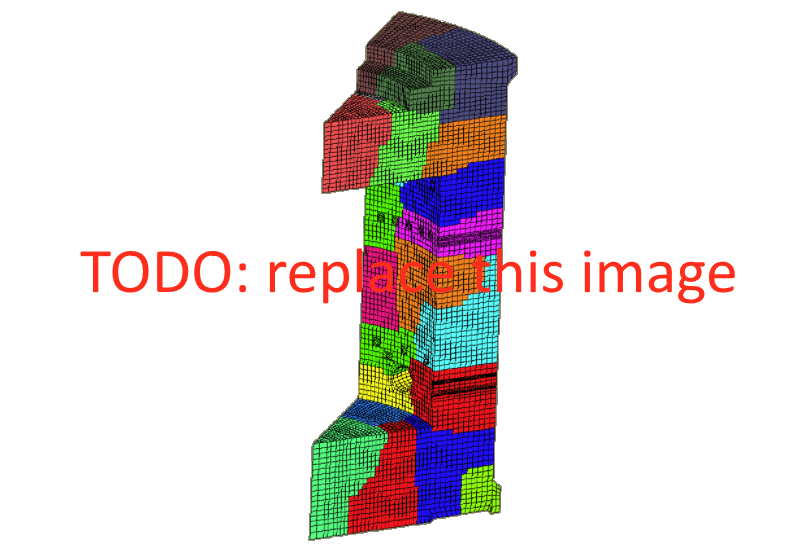
\includegraphics[width=\textwidth]{figures/chapter-introduction/motivation-example}
\decoRule
\caption[TODO: ]{TODO: Motivation example visualization}
\label{fig:motivation-example}
\end{figure}

The thesis is structured in the following manner. Chapter \ref{chapter:related-work} gives a brief revision of related work performed in FEA data management, file formats, data compression, and post-processing of the results. Chapter \ref{chapter:data-management} deals with the alternative to file-based data management. Section \ref{sec:system-architecture} contains proposal of relational database model that connects all parts of Finite element analysis including geometry, model attributes, and simulation results, providing query interface and remote access over the Internet. Section \ref{sec:storage-format} describes details of new data format. Section \ref{sec:postprocessing} presents design of the postprocessor that is built on top of the data management system. Chapter \ref{chapter-implementation} summarizes interesting technical details and challenges that arose during implementation of the management system and post-processor. Chapter \ref{chapter:overall-results} evaluates the implementation of the tools that are based on the new storage format and contains comparison to the traditional data formats. Chapter \ref{chapter:conclusion} concludes the thesis with final remarks, benefits and weaknesses of the chosen solution, and possible future work.

%----------------------------------------------------------------------------------------
%	SECTION Concepts
%----------------------------------------------------------------------------------------

\section{Concepts}

Here follows a summary of basic terms and concepts the thesis is based on.

\paragraph{Finite Element Method (FEM).} FEM is a numerical method for solving problems of engineering and physics. Typical areas include structural analysis, heat transfer, fluid flow, and electromagnetics. The analytical solution of these problems generally require the solution to boundary value problems for partial differential equations. The finite element method formulation of the problem results in a system of algebraic equations. The method yields approximate values of the unknowns at discrete number of points over the domain \cite{XXX}. To solve the problem, it subdivides a large problem domain into smaller, simpler parts that are called finite elements. This process is called the mesh generation \cite{XXX}. The simple equations that model these finite elements are then assembled into a larger system of equations that models the entire problem. FEM then uses variational methods from the calculus of variations to approximate a solution by minimizing an associated error function \cite{XXX}. The focus of this thesis is exclusively on the data management problems in the context of FEM-based simulations, not the simulations themselves.

% TODO: do predchoziho odstavce vlozit vysvetleni gaussovych/integracnich bodu

\paragraph{Finite Element Analysis (FEA).} Various data creation and modification tasks precede and follow the actual numerical solution of the boundary value problem using FEM. This whole process is called \textbf{Finite element analysis} and consists of several distinct phases. The basic phases of a FEA depicted in Figure \ref{fig:FEA-phases} are\footnote{This is a quite simplified description of the FEA process as the results from one simulation are then sometimes used as an input for other simulations. Preliminary results of the simulation can also be post-processed continualy during the calculation phase to monitor the convergence of the iterative methods. Another case represent the iso-parametric representation of finite elements \cite{XXX} and NURBS-enhanced FEM \cite{XXX}. These new approches are somewhat bridging the mesh generation phase as the curves describing the geometry are used also as the base functions of the finite elements.}:

\begin{enumerate}
    \item \textbf{Model creation} phase describes geometry of the domain, typically by defining boundaries of the domain using parametric surfaces like Bézier patches or Non-Uniform Rational Bézier-Splines (NURBS) \cite{XXX} in a CAD (Computer Aided Design) tool.
    \item \textbf{Attribute definition and assignment} specifies properties of the model, i.e. material properties of volumes, initial and boundary conditions for the solution.
    \item \textbf{Mesh generation} decomposes the geometry of the model into simple shapes (triangles or quadrilaterals) or voxels like tetrahedra or bricks that fill the volume. This is often only an approximation of the orignal domain, because it is not possible for these simple shapes to fill the complex domain completely without gaps.
    \item \textbf{FEM solution} uses the equations describing the problem, model discretization, and attributes to simulate the system's behavior. Often, the process is parametric either in geometry, or in assigned attributes. Simulation then produces multiple sets of output data, each for different configuration.
    \item \textbf{Post-processing} of results is examination of the output by engineer or scientist, who is seeking the features and trends in data using the visualization tool.
\end{enumerate}

\begin{figure}[H]
    \centering
    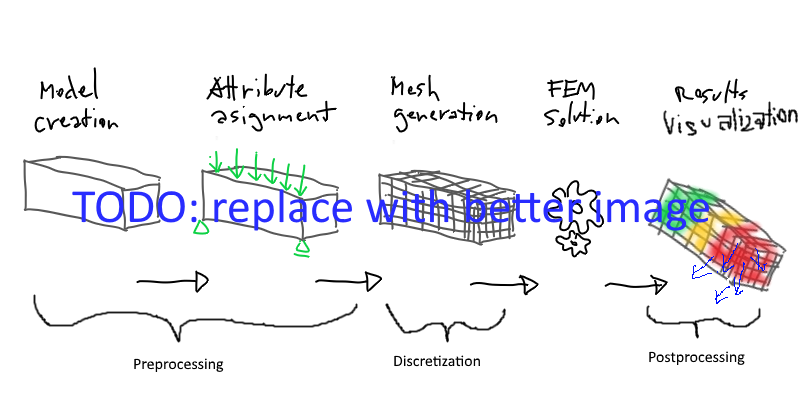
\includegraphics[width=\textwidth]{figures/chapter-introduction/FEA-phases}
    \decoRule
    \caption[TODO: ]{TODO: FEA phases}
    \label{fig:FEA-phases}
\end{figure}

Visualization tools are used to explore and analyse the data during all the phases. However, the vast majority of discussion about FEA focuses on the solution phase only. This makes sense as the solution phase consumes the largest portion of the computer time. But the solution phase itself consumes the insignificant amount of people-time. The majority of people's time is spent in pre-processing and post-processing of complex models. This fact seems to be overlooked and is one of the motivations for research work presented in this thesis.

\paragraph{FEM results.} Results from FEM are scalar, vector, or tensor fields represented by discrete values. Some results are stored in nodes of the mesh, such as vectors of nodal displacements. Other results are stored typically in Gauss points (i.e. integration points) on finite elements. There are two similar sets of results. One is generated by a non-linear algorithms, where several incremental steps are stored and the other is generated by time integration, where results in particular time steps are stored. These results are represented as dense tabular values of basic types, usually double-precision floating-point numbers (8 bytes each). For example, a 3D material stress calculation of the domain discretized by tetrahedral elements with quadratic approximation yields 12 values for the stress and strain tensors in each Gauss points. There are 11 Gauss points in each element. If 100 time samples are taken, the size of the solution output is $100 \times 12 \times 11 \times 8 \approx 100$ kilobytes per single (!) element. The number of finite elements depends on (1) the resolution of the discretization, (2) the geometric complexity of the model, and (3) the desired accuracy of output. In practice, fine discretizations of the problem domain contain millions of elements.

Current FEA software packages store the results either sequentially in formatted \textit{ASCII or binary files} ordered by time steps, or use more sophisticated \textit{database}\footnote{The term database is used here to describe any structured storage beyond a simple file store.} systems to preserve the links between the input model and the simulation results. Either way, the size of output data is very large for non-trivial analyses, which puts pressure on storage capacity, transfer times over the network, and memory consumption of postprocessing tools.

\paragraph{Data compression.} A compression method can be lossy or lossless. Lossless methods reduce information by identifying and eliminating statistical redundancy in data and are therefore able to fully reconstruct original data from its compressed form. Lossy methods, on the other hand, reduce the size by removing less important information in data and are thus producing only the approximation of original data.

\paragraph{Approximation error.} Compression methods usually yield approximated data. In the following text, the term approximation error denotes an error resulted from compression, i.e. difference between original results of FEM analysis and their compressed form. It should not be confused with the error of the Finite Element Method itself that yields approximate solution to mathematical problems used to model physical reality. There are defined several error metrics in the text (Section \ref{sec:error-estimation}) that are used to measure the approximation error.

% TODO: vysvetlit, proc pouzivam pojem Multi-mesh (Multigrid byla inspirace)

% TODO: pridat dalsi pojmy/hesla, ktera potrebuji vysvetlit. Tato kapitola by mela fungovat jako slovnicek pojmu

%----------------------------------------------------------------------------------------
%	SECTION Aims
%----------------------------------------------------------------------------------------

\section{Aims} % or Goal of the thesis

\begin{itemize}
    \item The main goal of the research work is to develop a new storage format that supports compression of results, and to outline the transition to a new post-processor that can read and visualize the compressed data in the new storage format. There is understandable resistance against invention of new data formats in the area of information technology. A new format leads to fragmentation of user base and compatibility issues. Conversion tools need to be created and maintained. There should be a strong motivation for introduction of a new format. However, there is no standard format for representation of results from FEM. Each software package uses proprietary format with syntax suitable for its internal implementation. There is also lack of support for compression methods that fit the character of FEM results. Standard file-based format does not allow for querying of specific information without the need to parse through the complete set of results. Chapter \ref{chapter:related-work} contains discussion about the existing formats in more detail and Chapter \ref{chapter:data-management} describes the proposed format.
    \item In addition, several suitable compression methods are proposed. Singular Value Decomposition (SVD) (Chapter \ref{chapter:SVD}) is the most promising method used for compression of results in this research. Other methods, that are investigated, include Wavelet transform (\ref{XXX}) and approximation of discrete values by continuous polynomial functions (Chapter \ref{chapter:approximation}).
    \item Finally, the product of this research is the implementation of two postprocessors. The first is a standard desktop postprocessor that is based on existing software and should present the way of transition from the convential file-based formats to the proposed structured database format utilizing compression. The second postprocessor is a web-based thin client intended to present advantages of the proposed format when incorporated into a complex FEA running on a remote server. Chapter \ref{chapter-implementation} summarizes implementation details.
\end{itemize}

%----------------------------------------------------------------------------------------
%	SECTION Challenges
%----------------------------------------------------------------------------------------

\section{Challenges}

Main challenge is a design of universal format that can hold the results from any FEM analysis. Results are composed of scalars, vectors, or tensors. Each field with different number of components. The results can be located on nodes or integration points. There may be a requirement to extrapolate the results from integration points to element nodes. There are different extrapolation strategies. Mesh can be different for each time step (e.g. in case of simulating the construction stages). Mesh can contain 1D, 2D, or 3D elements. Each of different type and approximation. Results from 3D simulations can be visualized on the surface of the mesh, in form of cross-sections or iso-areas, or as a vector field. The storage format should support efficient generation of all these views of results.

Finite element solution and post-processing of results can be sometimes done on different computers. Complex FEA solution phase runs on a supercomputer or a performant cluster of workstations, but the results are post-processed on common personal computer that has significantly less memory available. Typical personal computer has 8 to 16 GB of RAM available while the size of results can be in order of tens to hunderds of gigabytes. Also, the data to postprocess have to be first transfered over the corporate network or the Internet. These conditions indicate the need for partitioning of data into smaller chunks and/or compression of data.

The goal of compression methods is a significant reduction in size while preserving the quality (keeping the approximation error low). Unlike with image compression methods where the main aspect is the human perception of the reconstructed image the compression of FEM results should be able to guarantee the matematical acuracy of the approximations and the user should be able to specify a desired value of the approximation error. Another concern is the computation complexity of the compression algorithm. The compression will be performed only once after the solution phase is complete. The computational time should be order of magnitude lower compared to the solution phase. Decompression (reconstruction of the original data) should be very fast as it is supposed to be performed every time the data are post-processed on the end device, which can be ordinary PC or even mobile device. The ability to create animations should also be taken into account.

Other kind of challenge is to provide a data management system that will connect all the FEA phases, i.e. to provide links between the geometric model, the mesh entities, and the output values. A project typically encompasses multiple simulations, each with different input or solver parameters. Multiple users are usually involved in the project and the system should help them to cooperate during the preparation of the input and allow to share the output of the analysis. All these aspects influence the design of the data management system.

% TODO: Pridat dalsi vyzvy a namety. Napr.:
% Slo by propojit vypocet a zpracovani vysledku? Zminit multigrid.
% Co takhle nejak zohledit chybu aproximace FEMu, zohlednit ji pri kompresi a prezentovat ji uzivateli?

\chapter{Related work}
\label{chapter:related-work}

This chapter gives a brief revision of related research work that deals with visualization of finite element meshes and results from FEM, file formats used for representation of FEM data, compression methods, and FEA data management.

% TODO: State of the art and discussion about related work in the area of FEM results post-processing, storage formats, and cloud-based FEA.

\section{Data compression and visualization}
% Vrstva je koncept, ktery se vyskytuje i u jinych postprocessoru (napr. Simscale)

mesh compression:

surface mesh visualization (refinement/progressive meshes):
\cite{Gudukbay2002}
\cite{Vasa2011}
\cite{Alliez2001}
\cite{Maglo2012}
\cite{Valette2004}

\cite{Hoppe1996}

% Quite surprisingly, most of the existing algorithms mainly use only general compression techniques, such as entropy coding, quantisation, PCA or wavelet decomposition, while the inherent geometrical properties of the compressed surface remain unexploited. In this paper we focus on geometry specific optimisation: we extend the PCA-based dynamic mesh compression by optimising the order in which the mesh is traversed.

volumetric mesh visualization:
\cite{Ueng2004}, \cite{Robaina2010}

Iso geometric analysis + post-processing
\cite{Stahl2017}

3D graphics on the web:
\cite{Evans2014}
\newline
\cite{Hoppe1998}, \cite{Limper2013}, \cite{Maglo2012}, \cite{Lavoue2013}, \cite{Valette2009}, \cite{Charland2011}, \cite{Behr2012}, \cite{OpenCTM2010}, \cite{Mouton2011}, \cite{Marion2012}, \cite{Alliez2005}

% Data compression is a very wide area - image compression is related, fem data compression se nedela, VTK sice podpoduje kompresi ale obycejnou zip?
Image compression methods:
\cite{Lui2001}
\cite{Watson1994}

\section{File formats}
% univerzalni formaty pro vstupni geometrii:
IGES (Initial Graphics Exchange Specification) \cite{Groton2006}, STEP (STandard for the Exchange of Product model data) \cite{Pratt2001}

% http://blog.grabcad.com/blog/2014/10/14/get-over-iges/

% BREP, STL, ... formats; VRML

% OpenCASCADE
\cite{OpenCASCADE}

% Abaqus
\cite{Abaqus}

\cite{McHenry2008}  presents about 140 file formats for representation of 3D models...


% VTK format podporuje kompresi, ale bez znalosti obsahu dat. Pouze nejakou ZIP kompresi ci co. Neni to tak efektivni. Kazdy casovy krok ulozeny zvlast. Ale umi ukladat v ascii i binarne (base64 kodovani)



% pro vysledky: proprietary formats, VTK open source - used in scientific reasearch mainly, Gmsh - open, GiD - proprietary, Abaqus, ...

% zatimco pro reprezentaci geometrickeho modelu existuje spousta standardizovanych formatu, pro reprezentaci vysledku neexistuje otevreny univerzalni format podporujici kompresi. snad jen s vyjimkou VTK, ale ten ma sve nedostatky

% https://scicomp.stackexchange.com/questions/23882/what-is-a-common-file-data-format-for-a-mesh-for-fem

VTK: \cite{VTK2015}
Gmsh: \cite{Geuzaine2009}
GiD: \cite{GiDPostProcess}
Abaqus: 
\newline
\cite{Ivanyi2012}

% TODO: prozkoumat dalsi formaty pro ulozeni vysledku (vetsinou asi proprietarni, zadny standard neexistuje?)

\section{Web-based data management}

% citovat papery
\cite{Ari2013}
\cite{Yu2010}
\cite{Peng2003}
\cite{Heber2007I}
\cite{Heber2007II}
\cite{Weng2011}
\cite{Chen2008}

Paraview web: \cite{Jourdain2011}

% uvest Simscale
\chapter{FEA data management}
\label{chapter:data-management}

Together with growing complexity of finite element calculations, the importance of management of data produced by the calculations is increasingly emphasized in both industrial and research communities. As information is shared between multiple users, moved from one computer to another, and further transformed to enable different views over the data to enable inpterpretation of the information. Definition of persistent and standard representation of the data is therefore required as well as the corresponding data access system architecture that allows to query the data.

\section{System architecture}
\label{sec:system-architecture}

The prototype implementation of the FEA data management system is designed as a collaborative framework that can be accessed by users from different client devices. Figure \ref{fig:FEA-architecture} depicts the schema of the system architecture. System consists of several independent modules. The FEM calculation itself runs on a remote server as one of micro-services\footnote{TODO: micro-services} along with mesh generation service, results processing service, etc. These services are controlled by the application service that provides interface to the client applications in form of REST-ful web API\footnote{TODO: REST; REST-ful service; REST web API.}.

\begin{figure}[H]
    \centering
    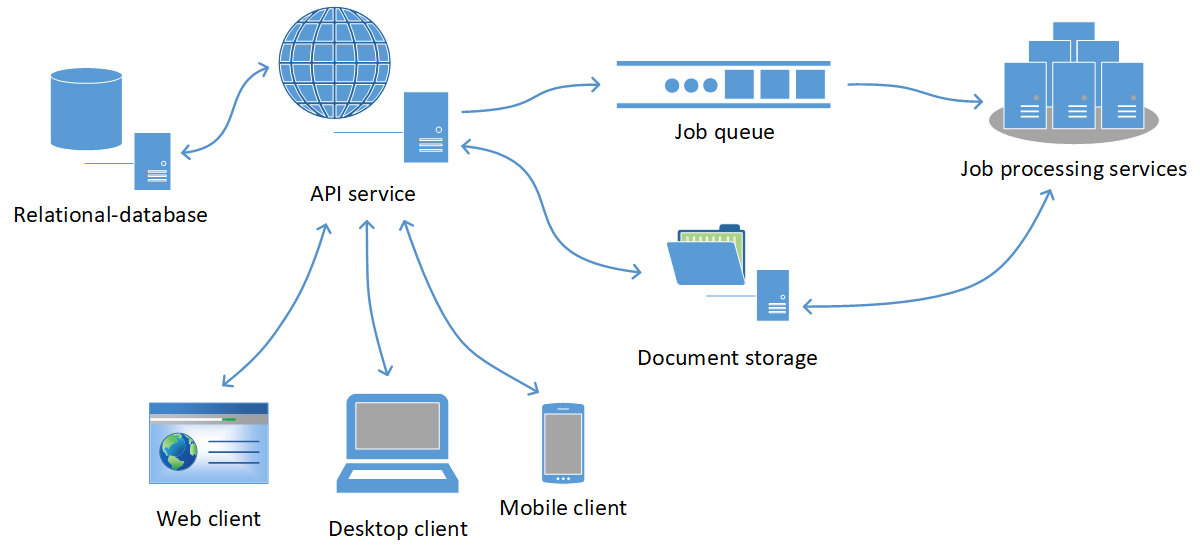
\includegraphics[width=\textwidth]{figures/chapter-data-management/FEA-architecture}
    \decoRule
    \caption{FEA system architecture.}
    \label{fig:FEA-architecture}
\end{figure}

The architecture relies on an abstraction provided by Platform-as-a-Service\footnote{PaaS. TODO: These services can be carried in a public cloud or on-premises. ...} computing model. No service component is tied directly to a specific machine. Hardware resources are allocated when they are needed by a service infrastructure controller. This makes the scaling and deployment of components easier and allows to focus on the problem domain instead of solving server configuration and networking issues.

The system contains two types of data storage. The relational-database type of storage is intended to store basic project-related data such as description of simulations, links to the simulation resources, information about the owner and other colaborating users, etc. The input to the FEA -- geometrical model, attribute assignments, and analysis parameters -- can also be stored in a relational database, eventhough, storing this complex type of information in the SQL database is questionable and has its drawbacks\footnote{TODO: Zminit vyhody i nevyhody. Jake jsou alternativy? No-SQL databaze?}.

The second type of storage is a blob storage used to hold temporary files serving as the input or the output to particular components, especially the mesh generator and the FEM solver. The system is designed to be independent of the solver and mesh generator components, therefore this intermediate step of converting the input to proprietary file format that the components understand is necessary. In the future, it is possible to expect a gradual transition from the file-based approach to the direct connection to the database and query the input model directly. Also, the output of the calculation could be saved directly in the proposed format to represent the results in post-process-ready form.

Workflow diagram in Figure \ref{fig:FEA-workflow} helps to visualize the sequence of FEA steps and the transfer of data between the service components. It also reveals the basic design principle behind the microservice architecture -- Separation of concerns\footnote{Separation of concerns -- design principle for separating system into distinct sections, such that each section addresses a separate concern.}. The vertical bars denote computational intensive tasks performed by the service components. The client side in the diagram represents the presentation layer of the FEA system that the user directly interacts with. In the presentation layer, also called \textit{frontend}, there is spent the vast majority of time by users doing pre- and post-processing of data (which is not depicted in the diagram). The Web API service, also called as \textit{backend}, is the key component that assigns work to other components, serves as an controller for a running analysis and mainly as an interface between the data stored in databases and the client applications.

\begin{figure}[H]
    \centering
    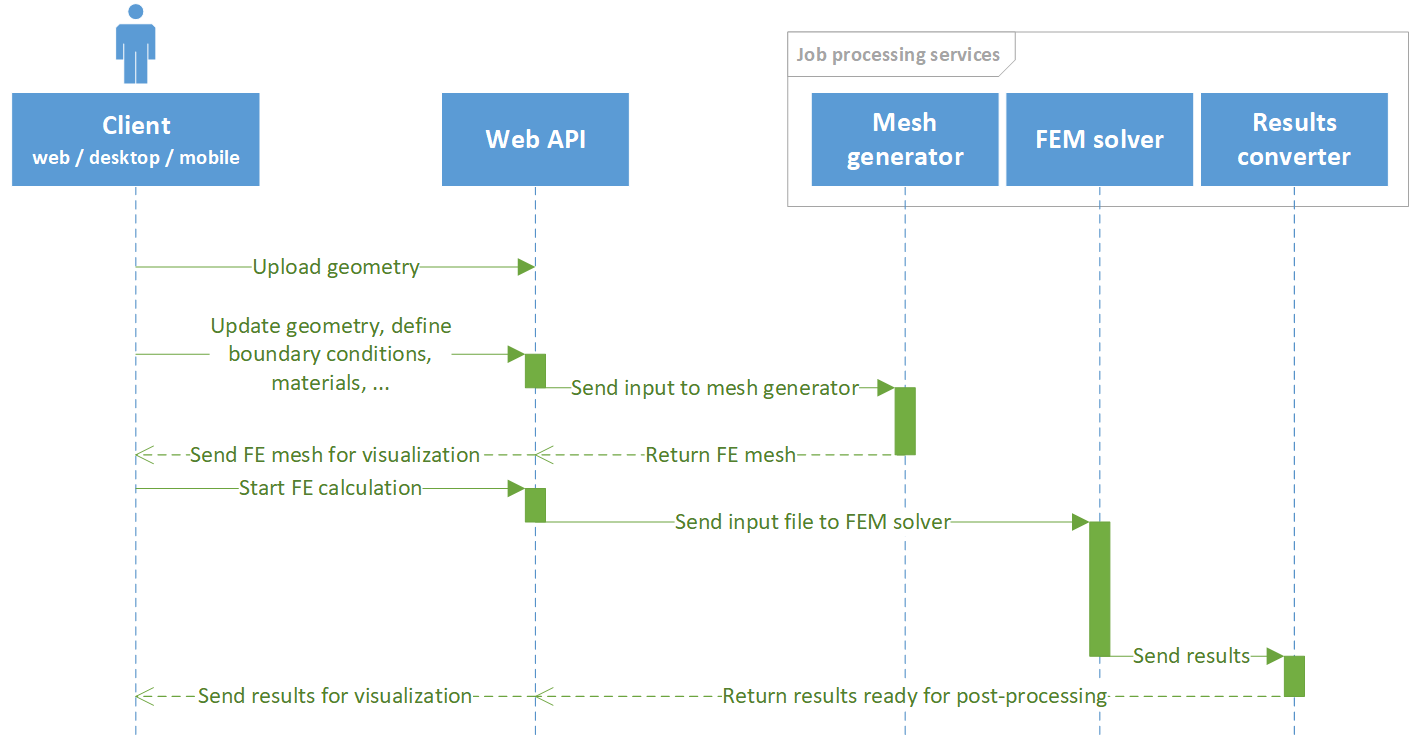
\includegraphics[width=\textwidth]{figures/chapter-data-management/FEA-workflow}
    \decoRule
    \caption{FEA system workflow.}
    \label{fig:FEA-workflow}
\end{figure}

The prototype implementation of the data management system follows the schema and the workflow depicted in Figures \ref{fig:FEA-architecture} and \ref{fig:FEA-workflow}. The difference is that the pre-processing phase is currently excluded. The focus of the work presented in this thesis is primarily on the post-processing features and the representation of results. Therefore, the results from the existing FEM solver are uploaded into the system and the system converts them to the internal representation suitable for post-processing. To test the prototype implementation of the data management system, two client applications are created. The first is the feature-rich desktop post-processor with the support for Microsoft Windows and Linux operating systems. The second is the simple web application that provides basic control over an analysis and basic post-processing capabilities. Its purpose is mainly to demonstrate the benefits of proposed format for storage of results when post-processing complex FEA. Its web-based implementation allows for truly cross-platform experience without the need for installation and it allows to access the analysis data even from low-end mobile devices.

\section{Project-based data representation}
\label{sec:project-db-schema}

Most researchers and engineers typically work independently using their own workstations, while sharing the hardware infrastructure for intensive FEM calculations. The output from the complex analyses are also shared as it would be costly and ineffective if each collaborator had performed her/his own calculations. Since potentially many users can access the server to oversee the analysis and to query the analysis results, a project management scheme is needed. The overall database schema is depicted in Figure \ref{fig:FEA-db-schema}. It is an entity-relationship diagram representing conceptual model that can be mapped on the SQL database model.

\begin{figure}[H]
    \centering
    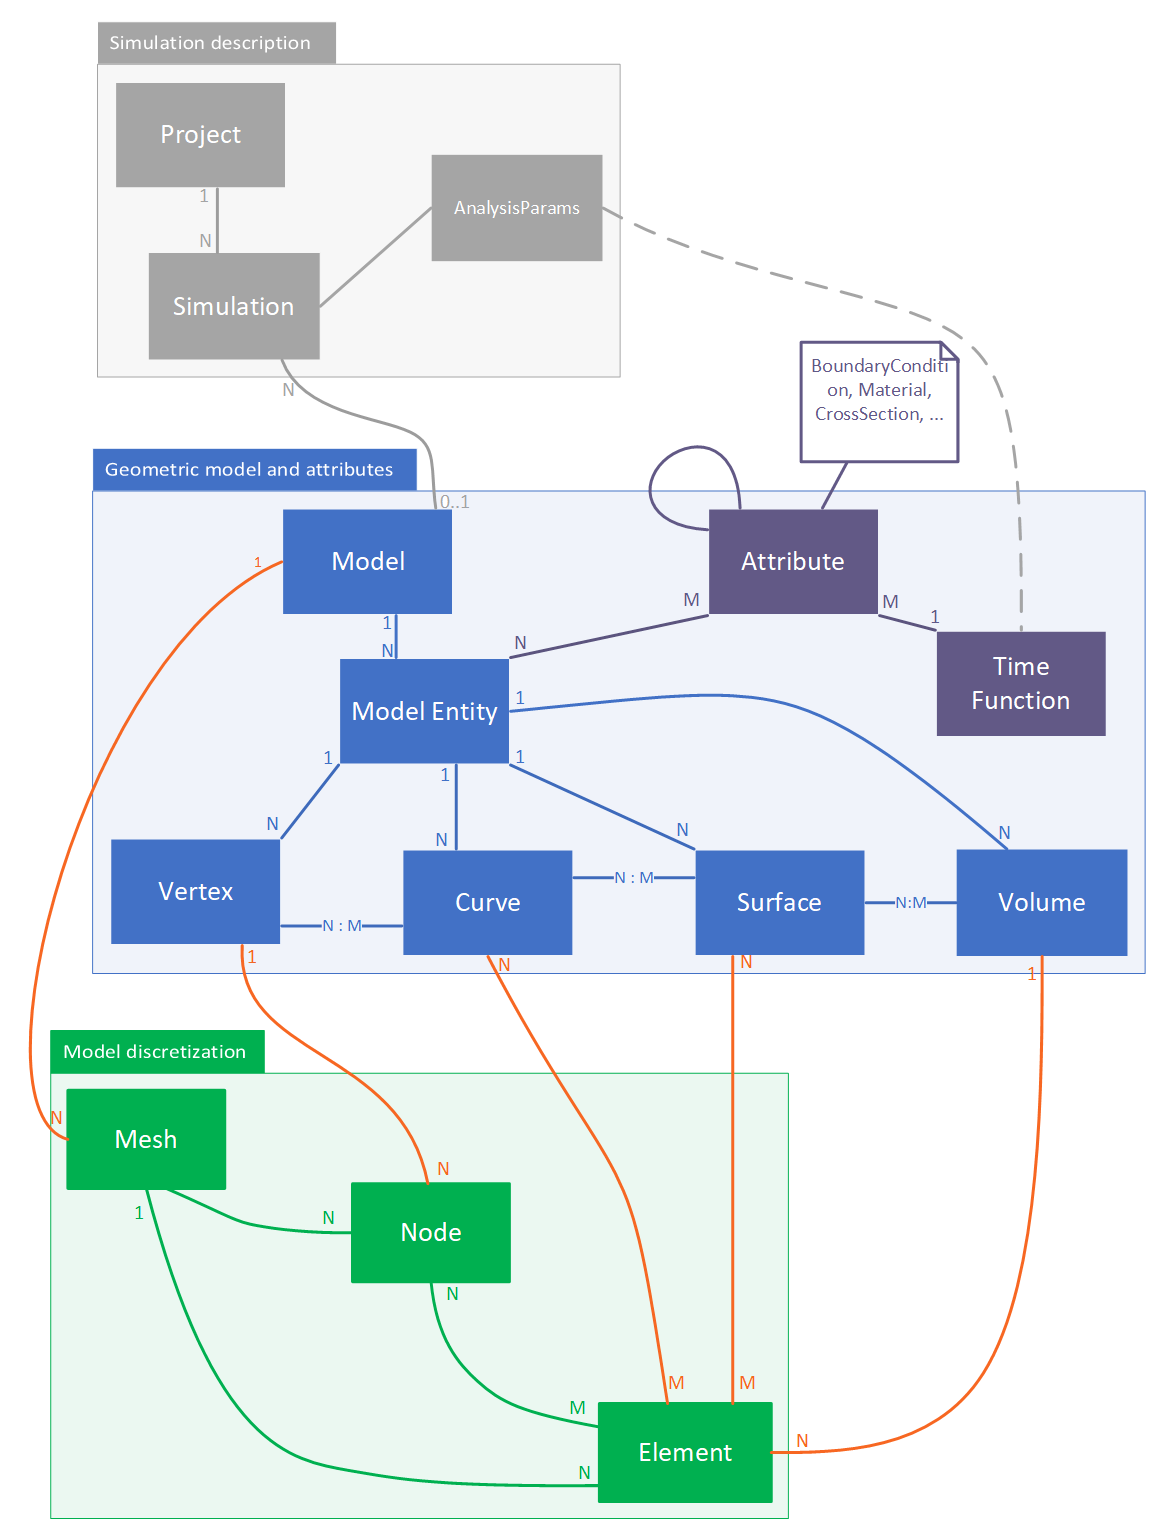
\includegraphics[width=0.8\textwidth]{figures/chapter-data-management/FEA-database-schema}
    \decoRule
    \caption{Database schema for FEA.}
    \label{fig:FEA-db-schema}
\end{figure}

The Project entity holds the basic information about a set of related analyses. It has name, the owner, and the list of other users that have access permissions. The Project has also relations to the list of simulations. The Simulation entity encapsulates the information about a single finite element analysis. Each simulation can have different input -- geometrical model, attributes (properties of model entities, i.e., material properties of volumes, initial and boundary conditions), and/or parameters of analysis (e.g., number of time steps). Geometrical model and its discretizations (finite element meshes) can either be stored directly in a relational database or as a custom file in a blob storage.

The conceptual model presented in Figure \ref{fig:FEA-db-schema} can be naturally extended to contain entities representing the results of the simulations. The project-based data model enhanced with the representation of simulation results is depicted in Figure \ref{fig:FEA-db-schema-results}.

\begin{figure}[H]
    \centering
    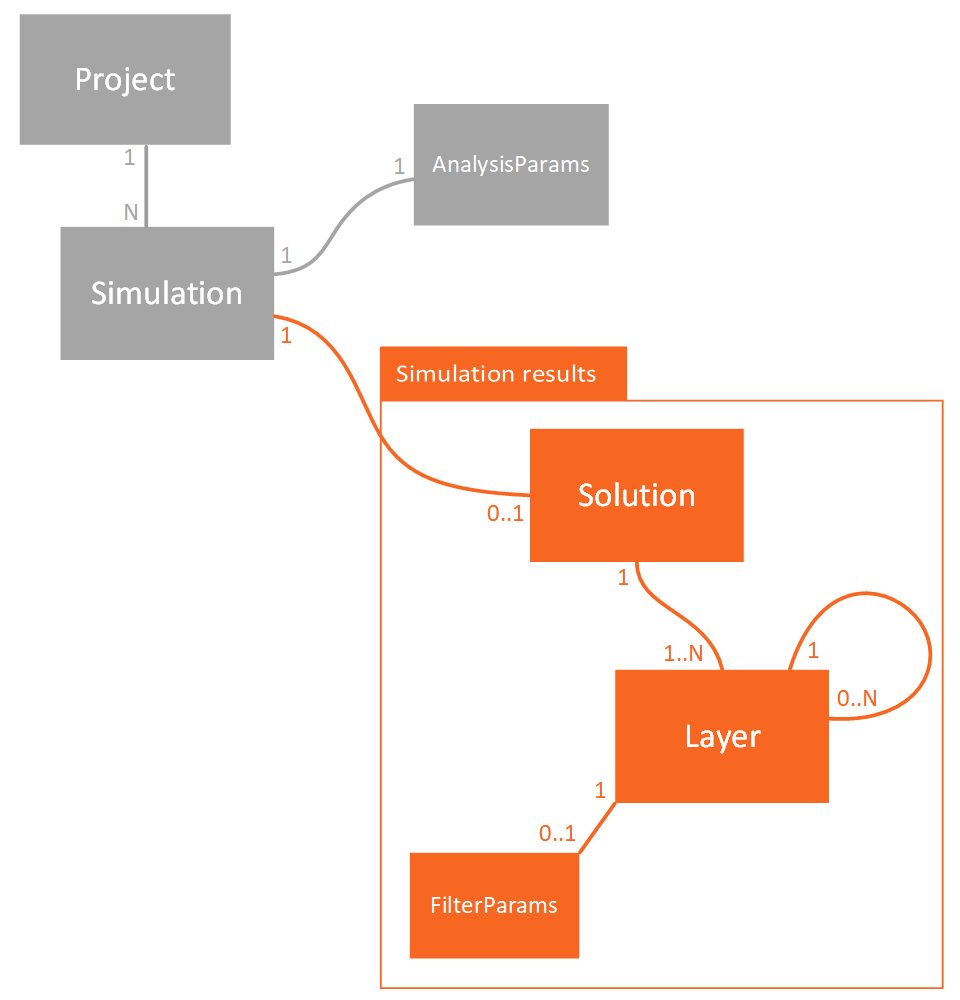
\includegraphics[width=0.6\textwidth]{figures/chapter-data-management/FEA-database-schema-only-results}
    \decoRule
    \caption{Database schema for FEA with results representation only (without the input model).}
    \label{fig:FEA-db-schema-results}
\end{figure}

The simulation results are represented by the Solution entity, which holds a structure representing the data generated by the FEM solver and converted to the form suitable for post-processing. The structure has the form of a tree with the nodes of type the Layer entity. A layer is an association of a mesh and corresponding result fields and other attributes. The mesh need not to be the same as the mesh used as the input mesh to FEM. It could be modified by the solver due to the use of adaptive finite element techniques \cite{XXX}, which can automatically refine, coarsen, or relocate a mesh to achieve a solution having a specified accuracy. Also, the resulting mesh can be further modified to facilitate the post-processing implementation, e.g. the surface representation of a 3D mesh can be generated as well as the cross-sections at uniform intervals. Generally, multiple views on the results can be prepared in advance before the user even starts to investigate the results. The concept of a layer is introduced to represent the pre-generated view and the tree structure allows to preserve the relations between the parent layers and the layers that were derived from them. More on the storage format for results is in the next section.


\section{Storage format for results}
\label{sec:storage-format}

% Pojmout tuto kapitolu jako detailni specifikaci formatu. Inspirovat se dokumentem GiD postprocess format (a take mozna C# proposals na githubu)

% Result converter component ma za ukol transformovat vysledky z FEM solveru do mojeho formatu (predpokladam pouziti solver komponenty, ktera ma vlastni proprietarni format, protoze se snazim navrhnout system nezavisly na jednotlivych komponentach)

% Centrem vseho je solution. To muze byt reprezentovano entitou v DB. Pripadne solution.json souborem v pripadne vysledku ulozenych a postprocessovanych lokalne. Hlavni koncept pri postprocessingu ke vrstva - layer - reprezentuje sit konecnych prvku a korespondujici vysledky at uz v uzlech ci v prvcich. Tyto data mohou byt zkompresovana. Vysvetlit, proc mam vic vrstev. Proc nestaci jedna.
% TODO: pridat obrazek stromu vrstev.

% In addition to that the desktop postprocessor ma moznost ukladat si data lokalne
% solution.json - priklad solution.json s layers tree - melo by nahradit fig:layers-tree - ten smazat?
% Remote/Local solutions - neni rozdil, postprocessor je tenky klient

Figure \ref{fig:layers-tree} ...

\begin{figure}[H]
    \centering
    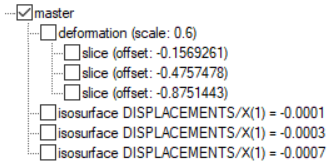
\includegraphics[width=0.5\textwidth]{figures/chapter-data-management/layers-tree-diagram}
    \decoRule
    \caption{Diagram of layer tree.}
    \label{fig:layers-tree}
\end{figure}

% samotny seznam souboru, ktere pouzivam. Nerikat tomu soubory, ale dokumenty? objekty?
% summary.json, mesh.json, attribute.json, and result.json - odkaz do Appendixu na example
% NoSQL DB
% U kazdeho souboru

% konverze z tradicnich souboru do noveho formatu (do budoucna integrovat do solveru); data location Points/Cells/CellPoints, GP extrapolation

% sit je krome vstupu dulezita i u vystupu. je nutne zachovat 1:1 mapovani vysledku na sit

\subsection {Encoding}
% base64, JSON, XML, ...

\subsection {Compression}
% Compression methods: SVD, Wavelet, polynomial functions, ... Kazdou rozepsat, u Wavelet zminit Hilbert curve?
% main features for optimization: key time steps (time step span compression), Randomized SVD, Parallelization, Sparse matrix of details, prenasobeni U matice singularnimi cisly, trochu usetrim pamet, mohu pouzit vzorkovani...

\section{Post-processing}
\label{sec:postprocessing}

% V teto kapitole popsat navrh post-processoru, ktery je postaven na popsanem datovem formatu
% layers, filters, vytvoreni Surface vrstvy pro webovy postprocessor, barevna skala, prepinani skalarnich velicin, vektorove veliciny - je treba nacist vice komponent najednou. Dekomprese: prenasobeni matic - staci jeden radek. ...

% ke kazdemu typu filtru pridat obrazek z postprocessoru at je to zajimavy

Displacement in Z axis: Figure \ref{fig:beam-master-layer} and Figure \ref{fig:beam-deformation-layer}.

Displacement in X axis: Figure \ref{fig:beam-slice-layers} and Figure \ref{fig:beam-isosurface-layers}.

\begin{figure}[H]
    \centering
    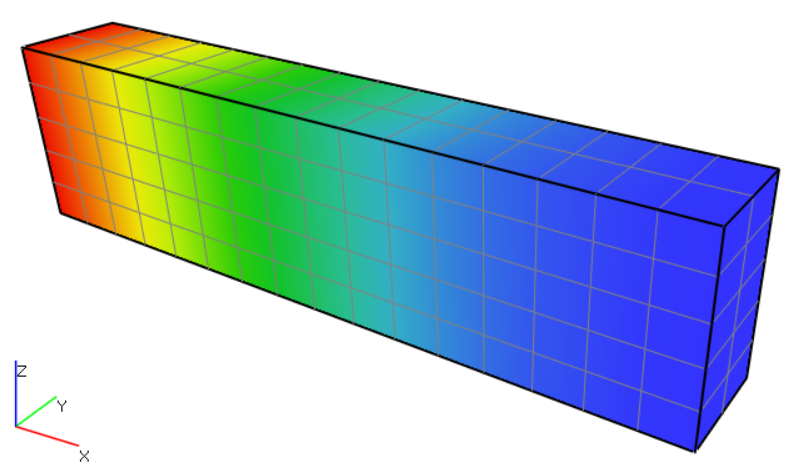
\includegraphics[width=0.7\textwidth]{figures/chapter-data-management/beam-master-layer}
    \decoRule
    \caption{Example of the master layer visualization.}
    \label{fig:beam-master-layer}
\end{figure}

\begin{figure}[H]
    \centering
    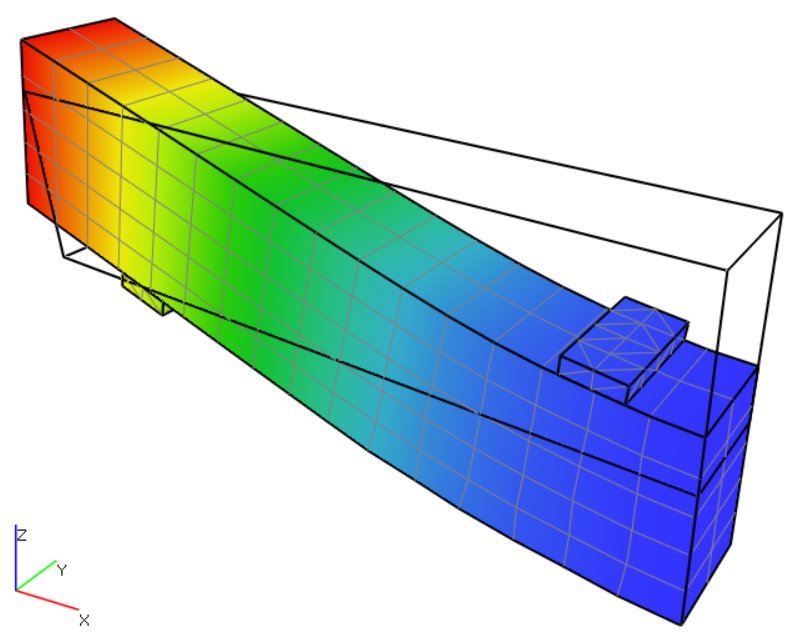
\includegraphics[width=0.7\textwidth]{figures/chapter-data-management/beam-deformation-layer}
    \decoRule
    \caption{Example of the deformation layer visualization.}
    \label{fig:beam-deformation-layer}
\end{figure}

\begin{figure}[H]
    \centering
    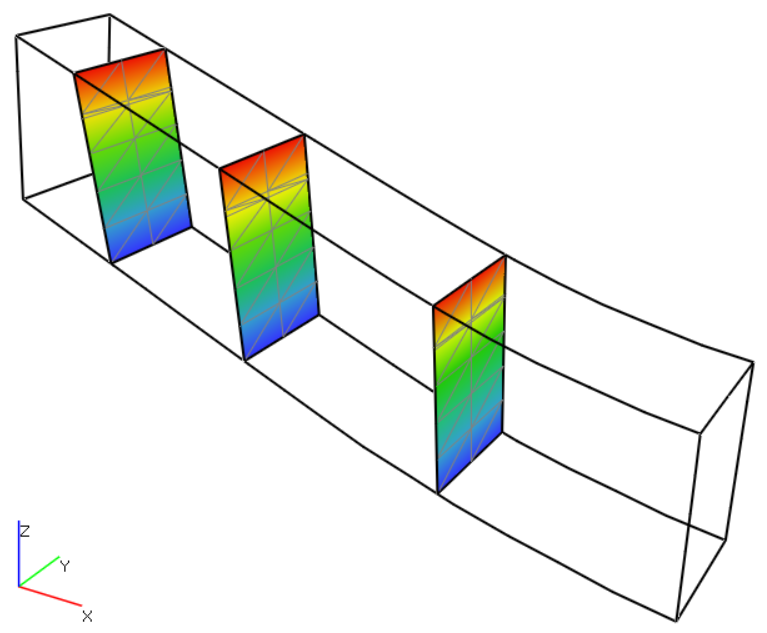
\includegraphics[width=0.7\textwidth]{figures/chapter-data-management/beam-slice-layers}
    \decoRule
    \caption{Example of multiple slice layers.}
    \label{fig:beam-slice-layers}
\end{figure}

\begin{figure}[H]
    \centering
    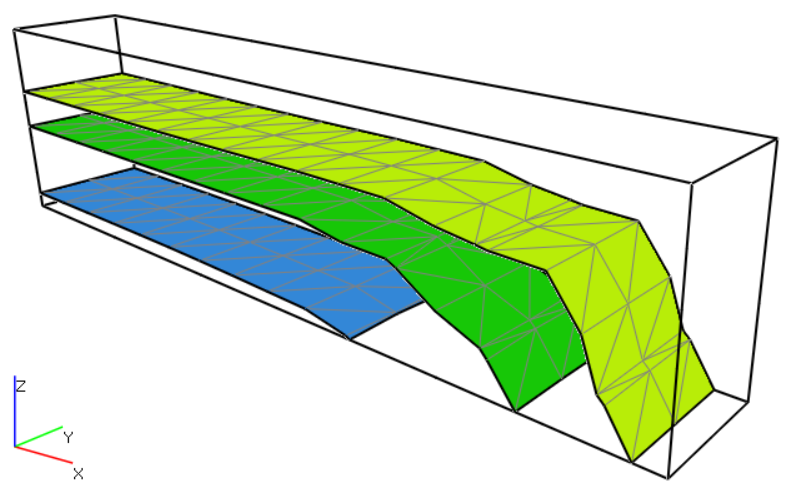
\includegraphics[width=0.7\textwidth]{figures/chapter-data-management/beam-isosurface-layers}
    \decoRule
    \caption{Example of multiple iso-surface layers.}
    \label{fig:beam-isosurface-layers}
\end{figure}


\section{Implementation details}
\label{sec:implementation-details}

% implementation details; cloud-infrastructure, Azure functions, web frontend, backend providing project info, blob-storage with layer format; command-based console management - popsat prikazy; reference to appendix with storage format examples
% SVD compression using redsvd; How is realized postprocessing of compressed data
% Encoding: converting to text representation, base64, NaN values, ... UTF8

% Webový browser, WebGL, textové pole se zadáváním příkazů, veškeré zpracování příkazů na serveru, na klient se budou posílat jen grafické buffery

% Přidat podkapitolku o implementaci barevné škály (diskrétní, spojitá, isoareas shader)

Figure \ref{fig:results-class-diagram} ...

\begin{figure}[H]
    \centering
    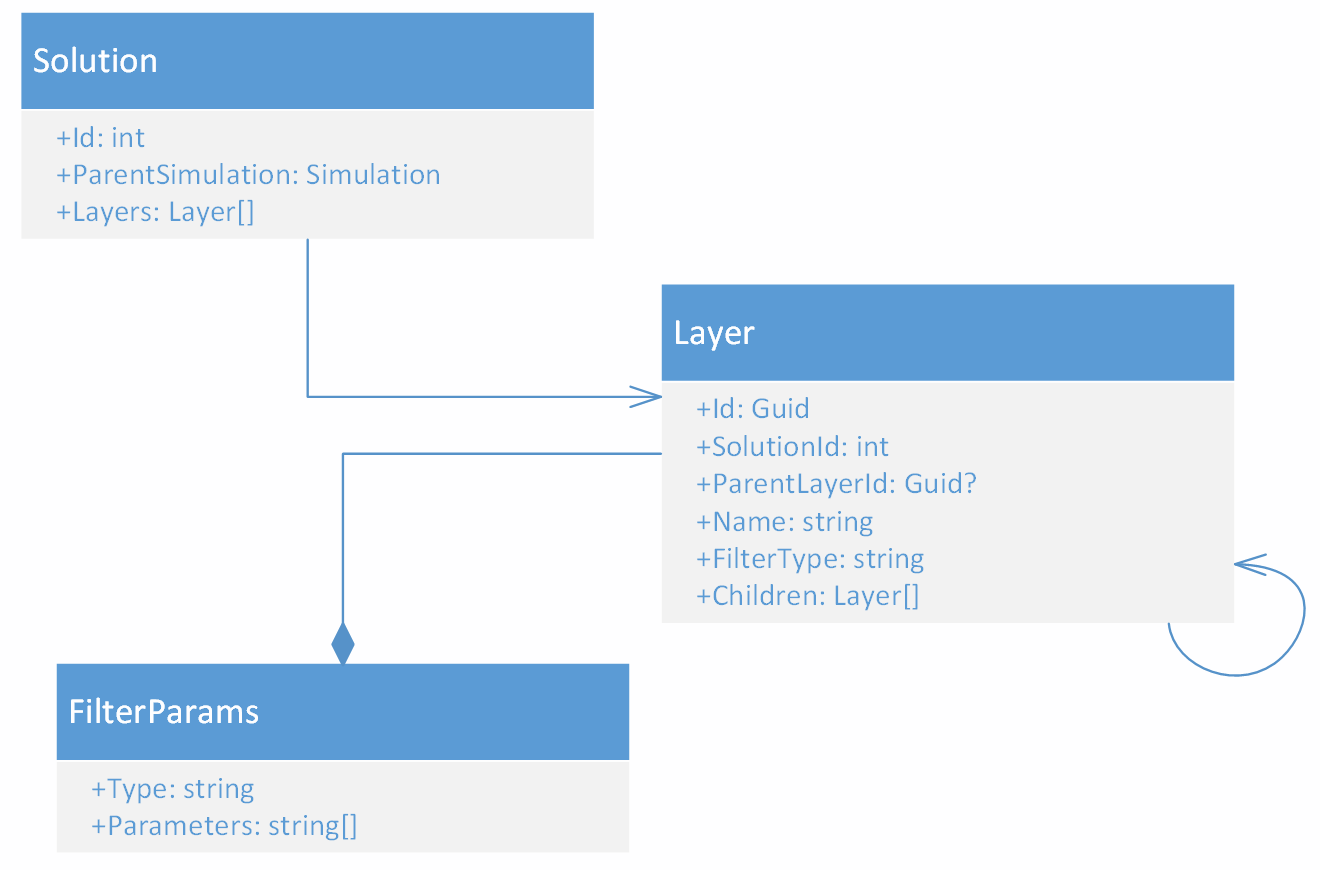
\includegraphics[width=0.7\textwidth]{figures/chapter-data-management/results-class-diagram}
    \decoRule
    \caption{Class diagram of results representation}
    \label{fig:results-class-diagram}
\end{figure}
\chapter{Efficient methods to visualize finite element meshes}
\label{chapter:mesh-visualization}

This chapter contains the description of the methods to process and visualize large finite element meshes and presents the design and implementation details of the desktop post-processor. The objectives for the implementation are high responsivness, comfort of use, and low memory consumption of the final application. The text in this chapter with more details is also published in \cite{Benes2015}.

%----------------------------------------------------------------------------------------
%	SECTION Theoretical background
%----------------------------------------------------------------------------------------

\section{Theoretical background}

It is needed to have the model of the problem domain as a composition of individual entities, their geometry and topological connections, before a finite element mesh is generated. The model is described by its boundary and the problem domain must be discretized for further use. This process is called mesh generation \cite{Frey2000, Rypl1998}. The output of a mesh generator is a finite element mesh corresponding to the input domain. The elements are the basic components and there are several types of them. The frequently used tetrahedral elements consist of four triangular faces described by three edges with the edge is made of two nodes.

It is sufficient to have only the list of nodes with their coordinates and the list of elements with references to their respective nodes for the mesh representation. Other entities (e.g. faces, edges) are usually omitted from the mesh generator output. However, the mesh editor has to handle them all, therefore, they must be created while loading the mesh. It is necessary to know all the kinds of the meshes that can be used as an input for the mesh editor implementation and especially for the design of the internal mesh representation. Meshes can be divided into several groups according to different criteria. The mesh classification is described in \cite{Hoppe1996}. The most basic form of mesh classification is based upon the connectivity of the mesh: structured or unstructured.

\textbf{A structured mesh}, also known as a grid, has a regular internal structure. Elements in the mesh are simply addressable due to the uniform distances between nodes. It restricts the element choices to quadrilateral in 2D or hexahedra in 3D. The regularity of the connectivity allows us to conserve space since neighborhood relationships are defined by the storage arrangement.

\textbf{An unstructured mesh} is characterized by irregular connectivity. It allows for any possible element that a solver might be able to use. When compared to the structured meshes, the storage requirements for an unstructured mesh can be substantially larger since the neighborhood connectivity must be explicitly stored.

Other mesh classification is based upon the \textbf{dimension} and the type of elements present. Depending upon the analysis type and solver requirements, meshes can be composed of one-, two- or three-dimensional elements. \textbf{Homogenous} meshes contain elements of the same type and dimension. \textbf{Hybrid} meshes are composed of elements of different type and/or dimension, e.g. tetrahedral mesh with 1D bars.

Additional classification can be made upon whether the mesh is \textbf{conformal} or not. An intersection of any two elements is either by a face, an edge or a node in conformal mesh. A non-conformal mesh contains for instance two quadrilaterals sharing two edges or two quadrilaterals sharing only a half of one edge. Non-conformal meshes are usually created during distributed generation of meshes from sub-domains and can cause issues during creation of the surface representation of non-conformal meshes. This issue is described in detail in section \ref{sec:A-implementation}.

Three-dimensional meshes can be replaced for the purpose of visualization with its surface representation. The elements (or parts of elements) that are hidden inside the volume of the mesh can be omitted. Visualization is much more efficient then. Most of the operations on entities, such as selection or setting of properties, can also be made on the mesh surface. The implementation of cuts through the volume is a problem. In order to show the entities on the cross-section, the surface representation must be regenerated each time. Making a cut is therefore a little more computationally intensive but it is outweighed by the fact that 2D surface representation is sufficient to handle any finite element mesh.

Because of the fact that the surface of both two-dimensional and three-dimensional elements is formed by either a triangle or a quadrilateral to represent the whole mesh, it is sufficient to use these two shapes. The surface representation must also include edges and vertices which the faces are formed of. The one-dimensional elements will be dealt with separately. When considering the internal representation of a mesh it is necessary to take into account the memory requirements. It should be noted that closed 3D mesh (not counting boundary elements) with homogenous structure and with $n$ elements has approximately $6n$ edges, $10n$ faces and $5n$ tetrahedral elements.

Most of the triangles and the edges will be inside the volume and can be therefore discarded after surface generation. The number of the surface entities is closely related to the geometrical shape of the domain. However, the number is significantly lower than the number of all entities for most meshes. The common operations on the mesh, e.g. to find neighboring faces, need complete topological data about the original mesh. The input file usually does not contain information about connections between elements. Therefore it must be determined while loading the mesh from the input file.

The data structure called \textbf{Winged edge} is used to store this kind of information. It is a widely used data structure in computer graphics especially for modeling practice, \cite{Baumgart1972,Floriani2005,Shirley2009}. It describes explicitly the geometry and topology of faces and allows fast traversing between faces, edges and vertices on the surface through a structure similar to the linked list. Traditional winged-edge data structure is represented by edge table. Each entry in the edge table contains these references: start vertex and end vertex, left face and right face, the predecessor and successor edges when traversing its left face, and the predecessor and successor edges when traversing its right face. Clockwise ordering (viewing from outside of the polyhedron) is used for traverse. Note that if the direction of the edge is changed, all entries in the table must be changed accordingly. Also, if some faces of a solid have holes, the above form of winged-edge data structure does not work. To make it work, ordering of the edges must be changed or some auxiliary edges must be added to surface representation. All these changes are difficult to implement efficiently. And this type of winged-edge data structure cannot be used for non-conformal finite element meshes. The basic composition of the winged-edge data structure that describes polygon meshes is widely used in computer graphics. However, the increased memory requirements compared to representations like the simple list of vertices and elements is the disadvantage. Moreover, the winged edge structure is based on dynamically created objects and therefore fragmentation of the memory can occur.

Figure \ref{fig:winged-edge} shows the adjusted data structure describing mesh surface based on traditional winged-edge schema, but eliminating some of its deficits. This structure is more suitable to use in finite element mesh scenario.

\begin{figure}[H]
\centering
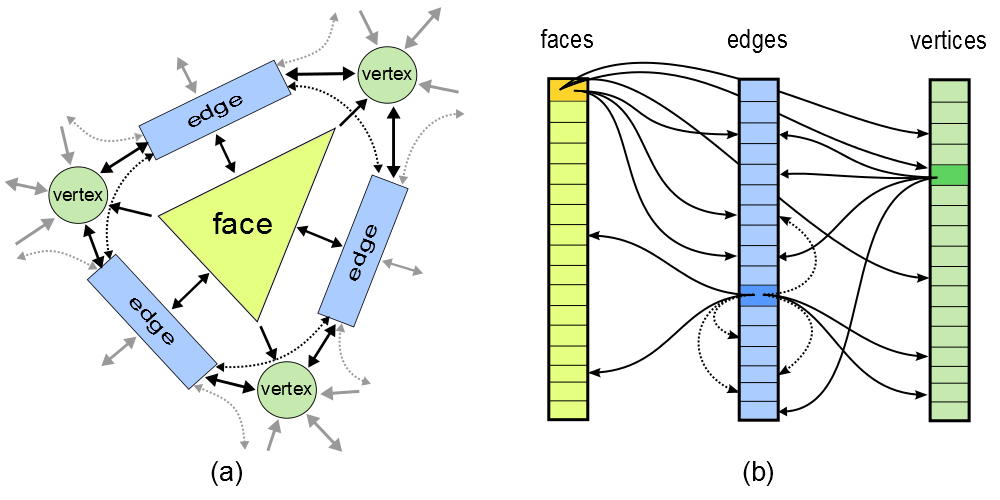
\includegraphics[width=\textwidth]{figures/chapter-mesh-visualization/figure1}
\decoRule
\caption[Winged edge data structure]{Winged edge data structure. (a) Entity dependencies. (b) Storage in lists with references.}
\label{fig:winged-edge}
\end{figure}


%----------------------------------------------------------------------------------------
%	SECTION Implementation details
%----------------------------------------------------------------------------------------

\section{Implementation details}
\label{sec:A-implementation}

All types of elements that are handled by the program are represented by the class hierarchy depicted in Figure \ref{fig:class-diagram-elements}. The common properties of all elements are accommodated in an abstract base class Element. The next level of the abstraction classifies the elements according to their spatial dimension. The particular class Beam stands for the one-dimensional element with linear approximation. The class inheriting from the Beam gains quadratic approximation by adding extra node in the middle of the line. The approximation type of other elements is distinguished by the type of their edges (a data structure describing the edge is similar to the one for 1D-elements).

\begin{figure}[H]
\centering
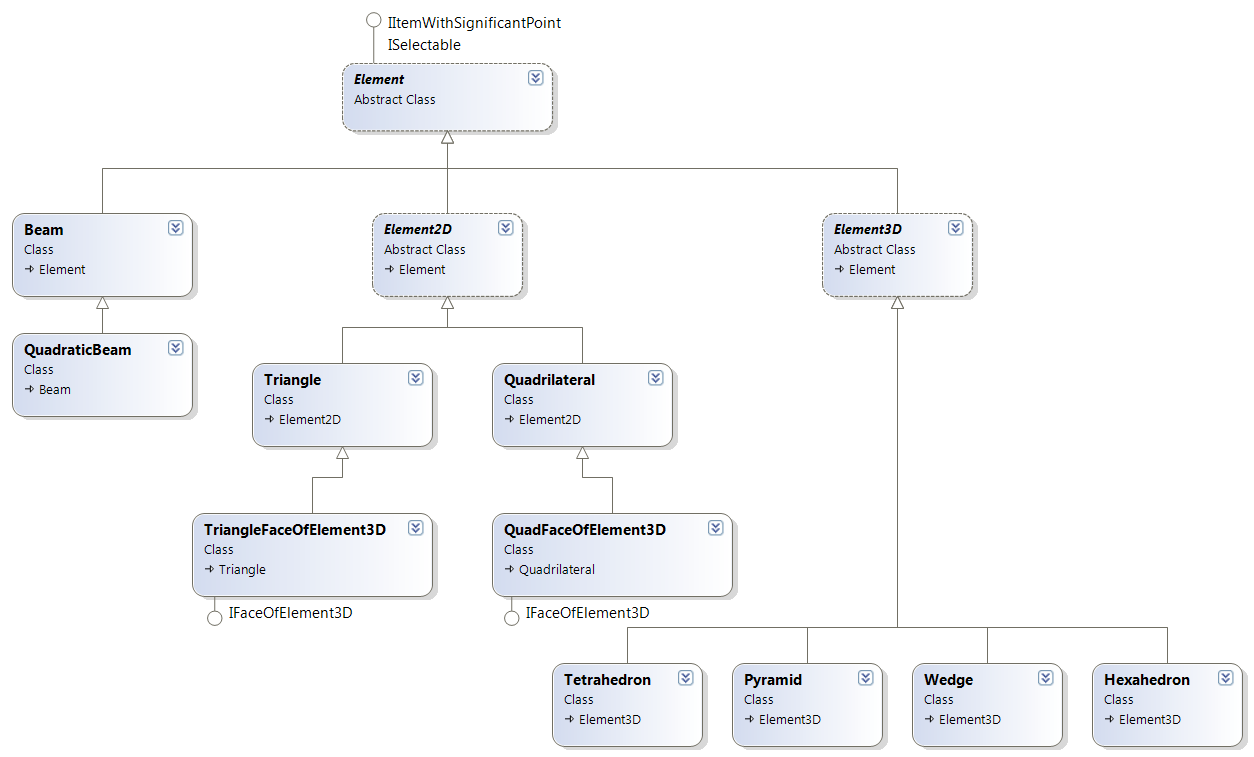
\includegraphics[width=\textwidth]{figures/chapter-mesh-visualization/figure2}
\decoRule
\caption[Class diagram of element types]{Class diagram with hierarchy of all supported element types.}
\label{fig:class-diagram-elements}
\end{figure}

The abstract base class Element2D is common for both the two-dimensional elements (triangle and quadrilateral) and faces of the three-dimensional elements (also triangles or quadrilaterals for all the widely used element types). The fact that 2D elements and faces of 3D elements can be handled in the same way allows us to implement a single generic algorithm for generation of the surface of the mesh so that the problem with hybrid meshes is hereby elegantly solved.

The 3D element face classes differ only by implementation of the interface \code{IFaceOfElement3D}.

\begin{lstlisting}
interface IFaceOfElement3D
{
	Element3D ParentElement { get; }
}
\end{lstlisting}

The interface helps to include reference to the parent 3D element at each face. This link is important for selection of elements on the mesh surface, because surface is composed, among other things, of external faces of those 3D elements that lie on the domain boundary. The adapted winged edge pattern is applied for the surface representation. All classes participating in this data structure are summarized in the class diagram in Figure \ref{fig:class-diagram-surface}.

\begin{figure}[H]
\centering
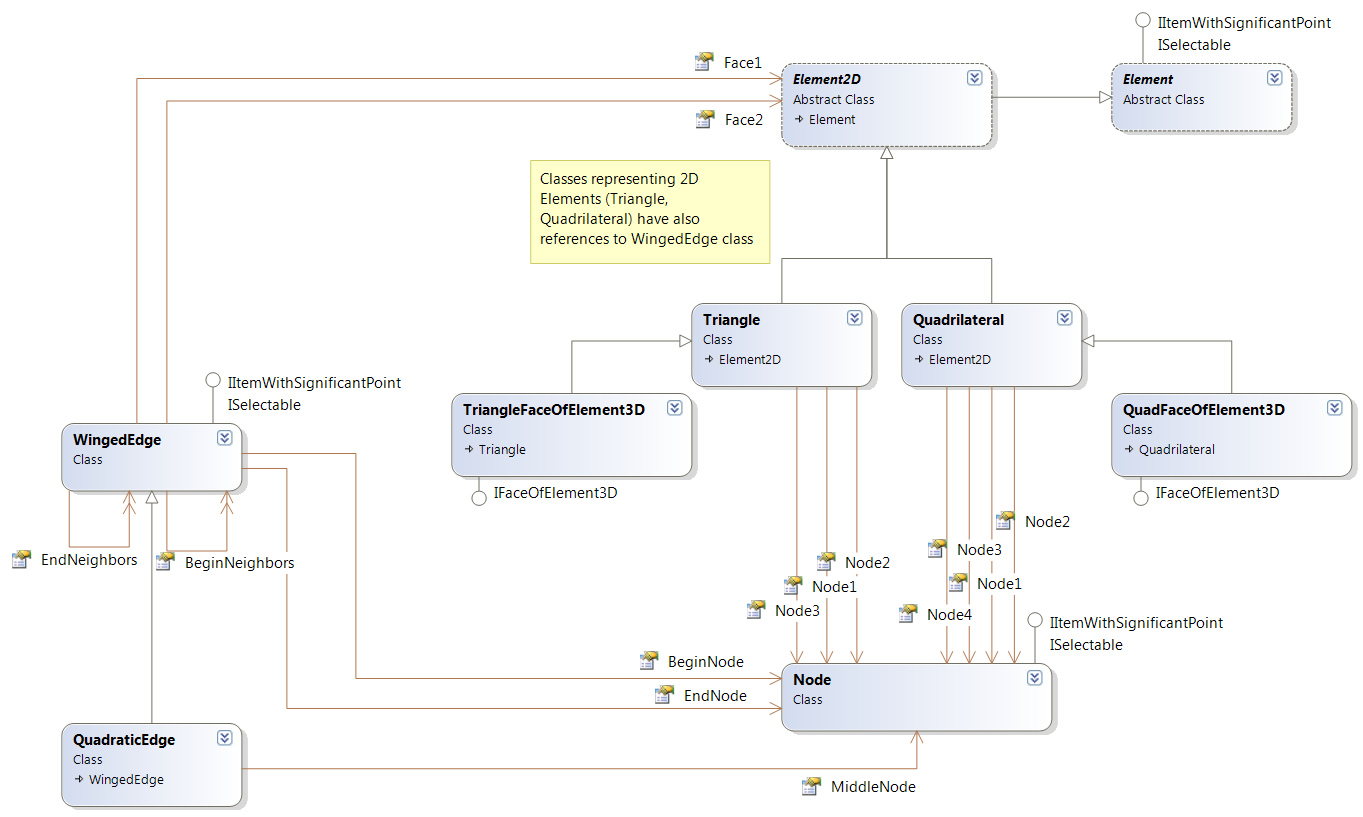
\includegraphics[width=\textwidth]{figures/chapter-mesh-visualization/figure3}
\decoRule
\caption[Class diagram of surface representation]{Class diagram with mesh surface representation.}
\label{fig:class-diagram-surface}
\end{figure}

Unlike traditional winged-edge data structure used in computer graphics in which each edge has references only to two neighboring edges, in our data structure each edge knows all its incident edges. The list of adjacent edges is tracked by every node and is shared between the node and all its neighboring edges. The ordering of edges in the list is arbitrary because in some cases there can be multiple candidates for its predecessors and successors. In this case no right ordering exists and traditional winged edge data structure used in computer graphics cannot be used. The surface representation is constructed on the fly in our single-pass algorithm. During the construction it cannot be known which edges are on the surface and what are its predecessors and successors. Therefore all adjacent edges for each node are kept in single unsorted list. To determine ordering of edges there would have to be second pass which would have significant negative impact on performance and therefore we wanted to avoid it. Moreover, for non-conform meshes there can be found no right ordering even after the surface construction.

Additionally, our approach has better memory footprint due to sharing adjacency list between node and all its neighboring edges as oppose to traditional winged edge structure. Another advantage is better performance in most common use cases of the mesh editor. Every user-triggered operation with mesh starts with selection of node or face on the mesh surface. Having direct references between each node and all its incident edges enables us quickly traverse the whole mesh surface.

Another adjustment of our data representation that differs from winged edge structure used in computer graphics is calculating and storing angle between each two neighboring faces. This enables us to implement advanced features such as finding significant edges or selection of logically related elements (e.g. on the same flat surface) as described below.

Besides the references to the begin- and end- nodes, every edge also has references to the lists of neighboring edges for each of both nodes. The lists are shared between the adjacent edges to achieve lower memory consumption. The edge also contains references to the faces on the left and on the right. This kind of linking is suitable for the majority of meshes. A problem can occur only in the non-conformal mesh processing when elements can share only a part of its surface. Visualization of this mesh can show up some artifacts caused by the fact that some internal faces do not have the adjacent counterparts and thus cannot be paired off. Another problem shows up when some elements have only one edge in common. In that case, the edge can be shared by more than two faces and the winged edge data structure cannot capture properly this situation. However, these are rare cases and do not render the program unusable.

%----------------------------------------------------------------------------------------
%	SUB-SECTION Data structures overview
%----------------------------------------------------------------------------------------

\subsection{Data structures overview}

The modified winged-edge data structure was used to describe the internal surface representation of a mesh. Instead of references to the left and the right adjacent edges, each node has reference to the list of all edges that begin or end at this node. The references to these lists are also contained in each winged-edge object. This approach allows representing the meshes with some abnormalities or non-conformal meshes in where it is impossible to determine which edge is the left and which is the right. Other characteristics of the winged-edge data structure remain the same. Each edge has references to the left and the right adjacent faces. Each face has references to its nodes, edges and the parent 3D element. The elements need to have references only to its nodes, because not every element is on the mesh boundary and so it does not need to have reference to surface objects. Every operation on the mesh, such as selection, begins with either a face or a node on the surface. Other entities are found by searching through the links in the winged edge data structure. Figure \ref{fig:data-structure-mesh} shows data lists used in the mesh editor.

\begin{figure}[H]
\centering
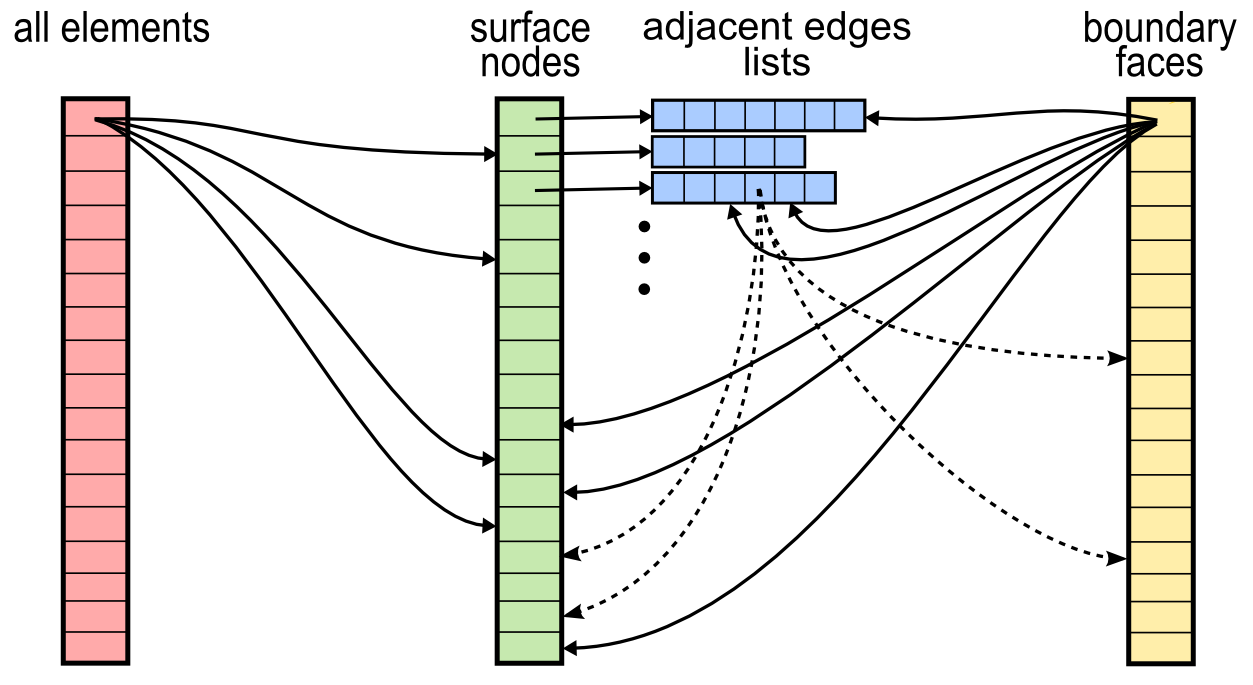
\includegraphics[width=\textwidth]{figures/chapter-mesh-visualization/figure4}
\decoRule
\caption[Data structure overview]{Diagram with data structure overview.}
\label{fig:data-structure-mesh}
\end{figure}

Memory requirements of each entity object are summarized in Figure \ref{fig:surface-rep-memory}. The overall memory consumption depends highly on the mesh topology and on the ratio of the number of surface elements to the total number of elements. This ratio decreases with the growing size of the mesh (or the element density) because the total number of elements increases with cube of the size of mesh, unlike the number of surface elements which increases with square of the mesh size.

\begin{figure}[H]
\centering
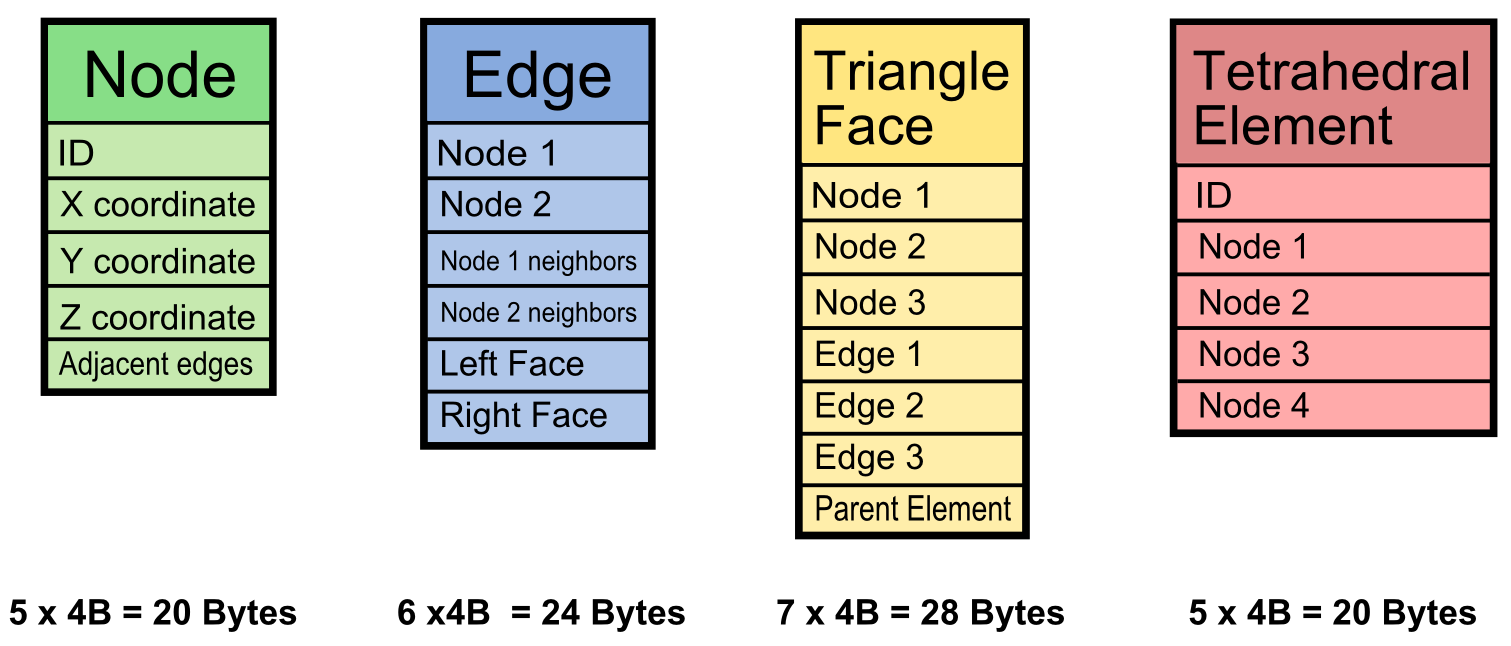
\includegraphics[width=\textwidth]{figures/chapter-mesh-visualization/figure5}
\decoRule
\caption{Memory consumption of the surface representation.}
\label{fig:surface-rep-memory}
\end{figure}

%----------------------------------------------------------------------------------------
%	SUB-SECTION Surface representation construction
%----------------------------------------------------------------------------------------

\subsection{Surface representation construction}

The process of creating the mesh surface representation is the key feature. It was designed as a one-pass algorithm which finds surface entities and creates the winged edge data structure on the fly during loading an input file. It should be noted that the input file does not contain any relationships between the mesh entities besides the coordinates of each node and a simple list of elements with links to relevant nodes.

The main problem is to find those faces of 3D elements that belong to the mesh surface. To resolve this issue we started with the consideration that each internal face has its twin in the adjacent element. While loading each element from the file, all its faces are generated. Then, the faces are included to a global hash table \cite{Knuth1998}. The key to this table is a special object consisting of the face node IDs. If the face under same key already exists, it means that the face is an internal face that we do not consider. Hence, the face is thrown away and the twin face is removed from the hash table. The procedure is repeated until all faces of all elements are processed. At the end (for conformal meshes) it is guaranteed that all remaining faces in the table are on the mesh boundary. For non-conformal meshes the algorithm can produce also some internal faces. Additional check for these situations is possible but it would break the simplicity and performance of the algorithm. Figure \ref{fig:mesh-construction} shows a diagram with the progress of loading an input file and constructing the mesh internal representation.

\begin{figure}[H]
\centering
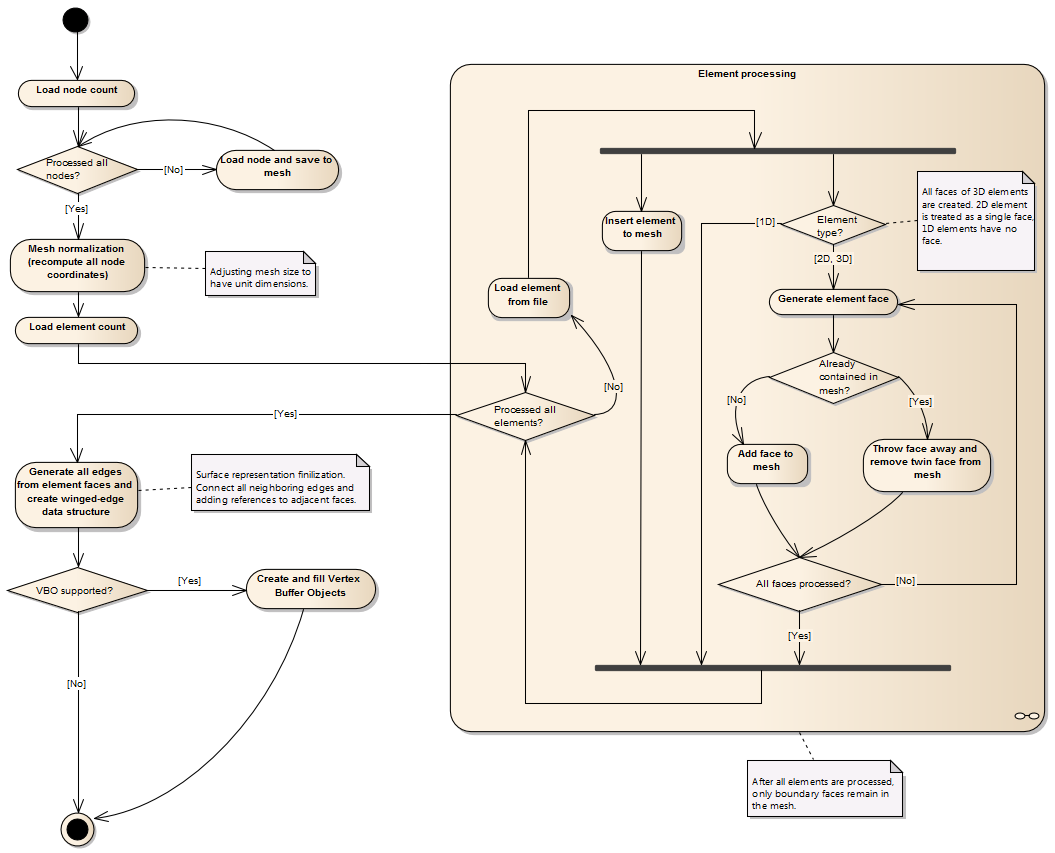
\includegraphics[width=\textwidth]{figures/chapter-mesh-visualization/figure6}
\decoRule
\caption[Activity diagram of mesh construction]{Activity diagram of loading and construction mesh surface representation.}
\label{fig:mesh-construction}
\end{figure}

In order to complete the surface representation, the edges must be generated from their faces. The analogous procedure that works with the hash table of edges is used here. Each edge has its twin in the adjacent face on the surface. But only one representative is needed. If a new edge is included into the table and under the same key the object is already contained, the new edge is thrown away. But compared to the previous case the edge in the table is not removed. The byproduct of this algorithm is finding the edges on the surface boundary. These edges have no twins as they have only one neighboring face. This however applies only to two-dimensional meshes, since the 3D meshes have a closed boundary.

Finally, when all surface entities are found, the Vertex Buffer Object (VBO) is created. It is an OpenGL feature that provides methods for uploading vertex data to the video device for rendering. VBO offers substantial performance gains over the immediate mode rendering because the data resides in the video device memory rather than the system memory and so it can be rendered directly by the video device. However, the buffer of rendered data must be updated each time the surface geometry changes. All up-to-date video cards support the VBO feature. If the card still does not support this feature, the application is smart enough to use the immediate-mode for rendering.

%----------------------------------------------------------------------------------------
%	SUB-SECTION Looking inside the mesh
%----------------------------------------------------------------------------------------

\subsection{Looking inside the mesh}

The editor allows to hide (or delete) some group of elements to enable the user to look inside the mesh. This makes sense especially for the 3D models when the user wants to see and manipulate the internal entities. Let us suppose that the set of elements to be hidden is known. Firstly, the program disposes of the current mesh surface representation and after that it basically creates the entire surface again with the use of the above mentioned effective surface representation construction algorithm. However, in this case the algorithm does not take all the elements from the input file as an input parameter, it take only those that are \textbf{not} contained in the list of elements to be removed. This solution offers the possibility to reuse the existing code that is already optimized and universally applicable to all types of meshes.

Moreover, this approach simplifies the implementation of other useful features summarized in the following list (all the features use the same surface construction algorithm).

\begin{itemize}
	\item \textbf{Hide selected elements} -- remove a set of arbitrary elements selected by the mouse pointer.
	\item \textbf{Show or hide elements with specific property} -- e.g. turn on or off layers containing elements with the same material id.
	\item \textbf{Cut through the mesh defined by plane} -- hide all the elements that are located behind the plane specified with three points lying in the plane or by a point on the plane and a normal vector. In this case only the elements that fall entirely behind the cut plane are displayed. Then the view is not perfect, but this approach is needed in our editor, where we have to assign properties to individual entities such as nodes and faces of elements. If the cut portion of the elements intersecting the cut plane would be displayed, editing of entities on the cut will not be possible. Also the implementation would be more complicated and our winged-edge data structure could not be used.
	\item \textbf{Cut through the mesh defined by general algebraic equation} -- previous operation (cut defined by plane) uses internal testing function that takes the point coordinates as an input parameter and returns a boolean value saying whether the point lies inside the area to be removed or not. The testing function is called for all currently visible elements. The testing function is in this case generalized to test the point against the algebraic equation specified by the user.
\end{itemize}

Each time the cut is performed the surface representation of the mesh is regenerated. Therefore turning on the cuts has no effect on the speed of manipulating views. All calculations are performed only during applying the cut through the mesh.

%----------------------------------------------------------------------------------------
%	SUB-SECTION Finding visible nodes
%----------------------------------------------------------------------------------------

\subsection{Finding visible nodes}

For various operations with a mesh, it is useful to have some method that finds the set of nodes that are visible from the current view-point, i.e. nodes that are not hidden behind a part of the mesh. Apart from the rendering of nodes and labels on the mesh surface, information about visible nodes can be used for implementation of the method for selection of entities on the surface using the mouse pointer.

The principle of the method is simple. Firstly, the method performs the perspective projection of all nodes to the screen and their actual depth is determined. Then the whole model is rendered into depth-buffer to produce a depth-map of the mesh. After that, the value in the depth-buffer corresponding to each node is compared to the Z-component of the screen coordinates of this node. If the value in the depth-buffer is greater than the projected distance of the node, the node is hidden behind some face. Otherwise, the node is added to the visible nodes set. The best precision in the depth-buffer is for the vertices that are in a small distance from the front clipping plane of the viewing frustum. The first step of the algorithm is therefore to move the near clipping plane from the observer to the mesh surface as close as possible. The pseudo-code of the described algorithm follows.

\begin{lstlisting}
Set<Node> FindVisibleNodes(Rectangle area)
{
	GL.MatrixMode(MatrixMode.Projection);
	GL.LoadIdentity();
	// move the Near plane closer to model for better precision
	double newZ_NEAR_PARAM = ComputeMeshMinVisibleDistance();
	// set perspective projection with updated parameters
	Glu.Perspective(FOVY_PARAM, aspect_ratio, newZ_NEAR_PARAM, Z_FAR_PARAM);
	// ---------------------------------------------------------------------
	// compute projections of all nodes to screen coordinates
	Dictionary<Node, Vector3> projections = new Dictionary<Node, Vector3>();
	Vector3 winPos;
	foreach (Node node in allSurfaceNodes)
	{
		Glu.Project(node.Position, modelview, projection, viewport, out winPos);
		if (area.Contains(winPos.X, winPos.Y)) // if the point is inside area,
			projections[node] = winPos;  // save projection to dictionary
	}
	// ---------------------------------------------------------------------
	// draw faces to depth buffer
	GL.Clear(ClearBufferMask.DepthBufferBit);
	GL.PolygonOffset(1f, 1f); // move little bit to enable testing
	GL.Enable(EnableCap.PolygonOffsetFill);
	DrawFaces();
	GL.Disable(EnableCap.PolygonOffsetFill);
	// ---------------------------------------------------------------------
	Set<Node> result = new Set<Node>();
	foreach (KeyValuePair<Node, Vector3> pair in projections)
	{
		Node node = pair.Key; winPos = pair.Value; float pixelDepth;
		GL.ReadPixels(winPos.X, winPos.Y, 1, 1, Format.Depth, Type.Float, out pixelDepth);
		// !! key depth test; if passes, node is visible
		if (winPos.Z <= pixelDepth)
			result.Add(node);
	}
	return result; // return list of visible nodes
}
\end{lstlisting}

%----------------------------------------------------------------------------------------
%	SUB-SECTION Selection of entities
%----------------------------------------------------------------------------------------

\subsection{Selection of entities}

The mesh editor implements a tool for selection of entities in the mesh. The tool has two modes. The first mode allows user to select entities contained in the rectangular area specified by dragging the mouse pointer. Implementation of this tool uses the above mentioned method \code{FindVisibleNodes()}. The set of nodes returned by the method is then transformed to the set of entities that the user wants to select by looking to the winged edge data structure that takes advantage of its rich interconnections. For example, if the user wants to select all the edges in the rectangular area, the algorithm finds all edges that have one of theirs node in the set of nodes returned by the method \code{FindVisibleNodes()} that takes the selection rectangle as a parameter.

The second mode of the tool is selection of some geometrically related entities, e.g. all nodes on the top of the mesh. The input file that is used does not contain any information about neither the model from which the mesh was generated nor the curves and planes that form the surface of the model. However, the user usually requests to be able to select such groups of entities.

The core of the implementation of this functionality is the method \code{SelectSurface()}. The method returns the set of element faces on the mesh surface that have pre-specified maximum angle between them. The angle (passed as a function parameter) defines the degree of smoothness of the resulting surface.

The limit angle is determined by the count of the mouse button clicks on some face. The target face is also passed as an input parameter of the function. The limit angle increases with a growing number of clicks. The program operates with four levels of tolerance in the surface selection. The default values of the limit angles for each level are carefully chosen to suit the largest number of the mesh. For atypical-formed meshes, the user can change these default parameters.

The following pseudo-code shows the implementation of the \code{SelectSurface()} method. Figure \ref{fig:element-face-selection} illustrates the result of the double- and triple-click on the mesh surface. Double-click selects all faces in the area that is delimited by the first limit angle. Default value of this parameter is one degree. Therefore double-click selects the elements or faces of elements which have a face on the same flat surface as the mouse cursor, whereas the triple-click selects the elements or faces on the smooth (possibly curved) surface as the mouse cursor. This surface is delimited by edges whose adjacent faces include angle lower than or equal to the second limit angle. Fourth click selects all the remaining neighboring elements or faces.

\begin{lstlisting}
Set<Element2D> SelectSurface(Element2D startFace, float borderAngleLimit)
{
	Set<Element2D> selectionSet = new Set<Element2D>(); // faces to select
	Stack<Element2D> faces = new Stack<Element2D>(); // visited faces
	faces.Push(startFace); // push starting face
	selectionSet.Add(startFace);
	while (faces.Count > 0) // while the stack is not empty
	{
		Element2D face = faces.Pop();
		// add to the stack all neighboring faces
		// that form with the face an angle of value at most borderAngleLimit
		foreach (Element2D neighbor in face.GetNeighbors(borderAngleLimit))
		{
			if (!selectionSet.Contains(neighbor))
			{
				faces.Push(neighbor);
				selectionSet.Add(neighbor);
			}
		}
	}
	return selectionSet;
}
\end{lstlisting}

\begin{figure}[H]
\centering
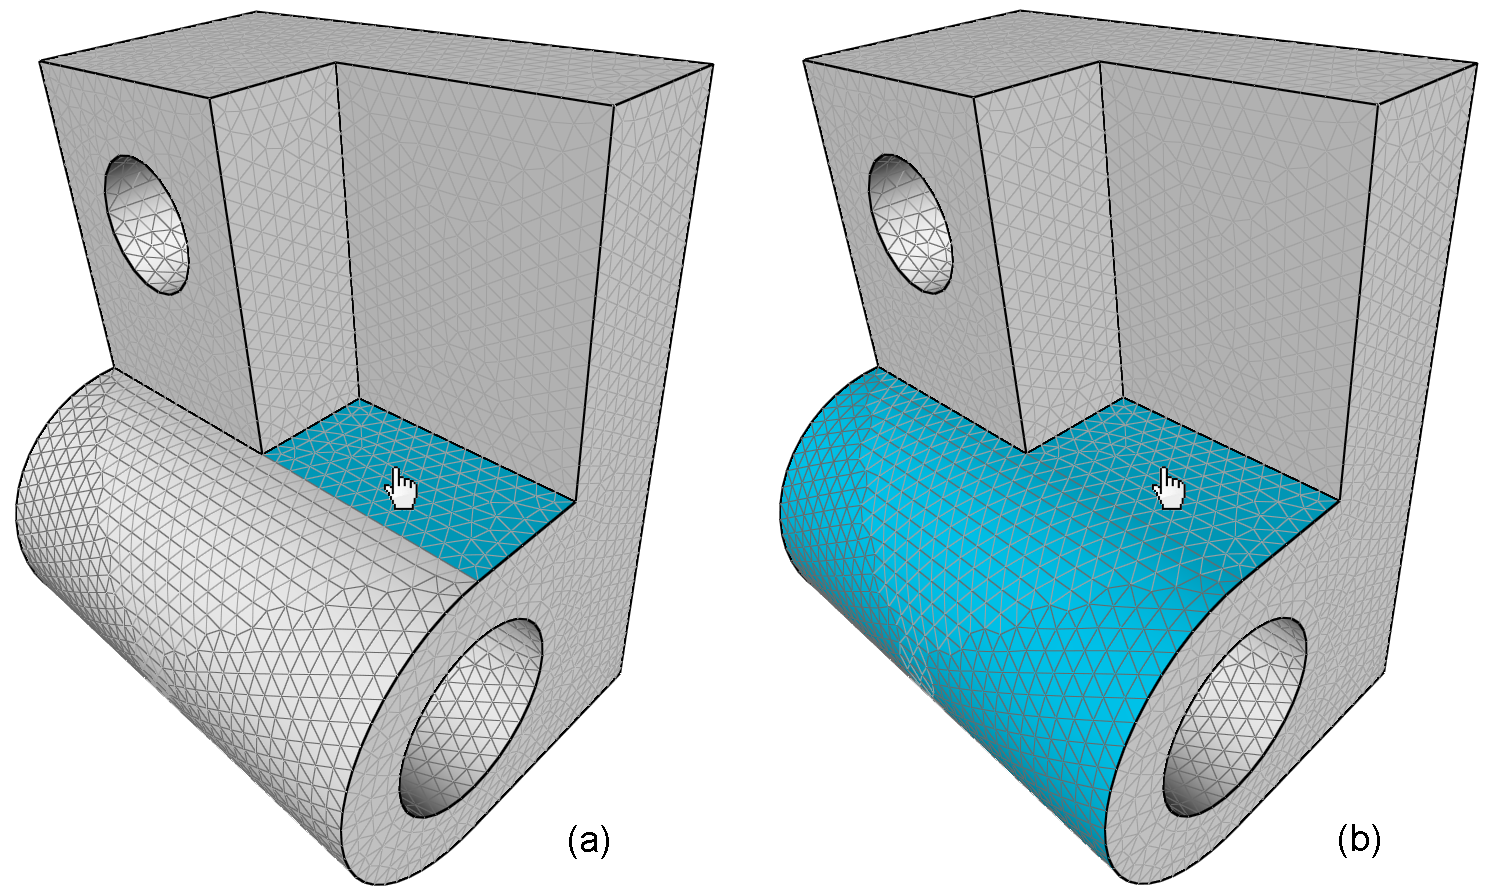
\includegraphics[width=\textwidth]{figures/chapter-mesh-visualization/figure7}
\decoRule
\caption[Selection of element faces]{Selection of element faces on the mesh surface. (a) Result after mouse double-click. (b) Result after mouse triple-click.}
\label{fig:element-face-selection}
\end{figure}


%----------------------------------------------------------------------------------------
%	SECTION Results
%----------------------------------------------------------------------------------------

\section{Results}

The program was benchmarked against other commonly used editors that have similar capabilities. We chose the \textbf{GiD} \cite{GiD2013} postprocessor, \textbf{ParaView} \cite{ParaView2005} and \textbf{VisIt} \cite{VisIt2005}. The initial loading time (see Table \ref{tab:loading-time}) and memory consumption were measured (see Table \ref{tab:memory-consumption}). The memory requirements of our mesh editor grows slightly faster than requirements of other tools for meshes with high number of finite elements. It is caused by auxiliary data structures assembled for future fast manipulation with meshes. The mesh Beam with $651.873$ elements represents a limit task which can be solvable on a single processor computer. For smaller problems, memory requirements of our editor are comparable or even smaller in comparison with GiD, ParaView and VisIt. Figure \ref{fig:benchmark-meshes} contains visualizations of the meshes that were used in the benchmark.

\begin{table}
\caption[Initial loading time comparison]{Measured results: Initial loading time in seconds (CPU time).}
\label{tab:loading-time}
\centering
\begin{tabular}{| l | r | r | r | r |}
\hline
\tabhead{mesh (size)} & \tabhead{MeshEditor} & \tabhead{GiD} & \tabhead{ParaView} & \tabhead{VisIt} \\
\hline
Beam (651873 elements) & 36 & 28 & 16 & 24\\
Beam (47680 elements) & 4 & 5 & 3 & 2\\
Beam (3222 elements) & 1 & 4 & 2 & 1\\
Sphere (348014 elements) & 4 & 3 & 7 & 2\\
Robo (244188 elements) & 7 & 7 & 7 & 7\\
\hline
\end{tabular}
\end{table}

\begin{table}
\caption[Memory consumption comparison]{Measured results: Memory consumption in megabytes (Private working set) [MB]}
\label{tab:memory-consumption}
\centering
\begin{tabular}{| l | r | r | r | r |}
\hline
\tabhead{mesh (size)} & \tabhead{MeshEditor} & \tabhead{GiD} & \tabhead{ParaView} & \tabhead{VisIt} \\
\hline
Beam (651873 elements) & 824.616 & 620.956 & 339.436 & 526.144\\
Beam (47680 elements) & 104.124 & 92.772 & 128.888 & 123.244\\
Beam (3222 elements) & 42.800 & 52.480 & 114.380 & 89.116\\
Sphere (348014 elements) & 108.324 & 106.428 & 133.652 & 128.808\\
Robo (244188 elements) & 291.836 & 200.484 & 543.316 & 355.268\\
\hline
\end{tabular}
\end{table}

\begin{figure}[H]
\centering
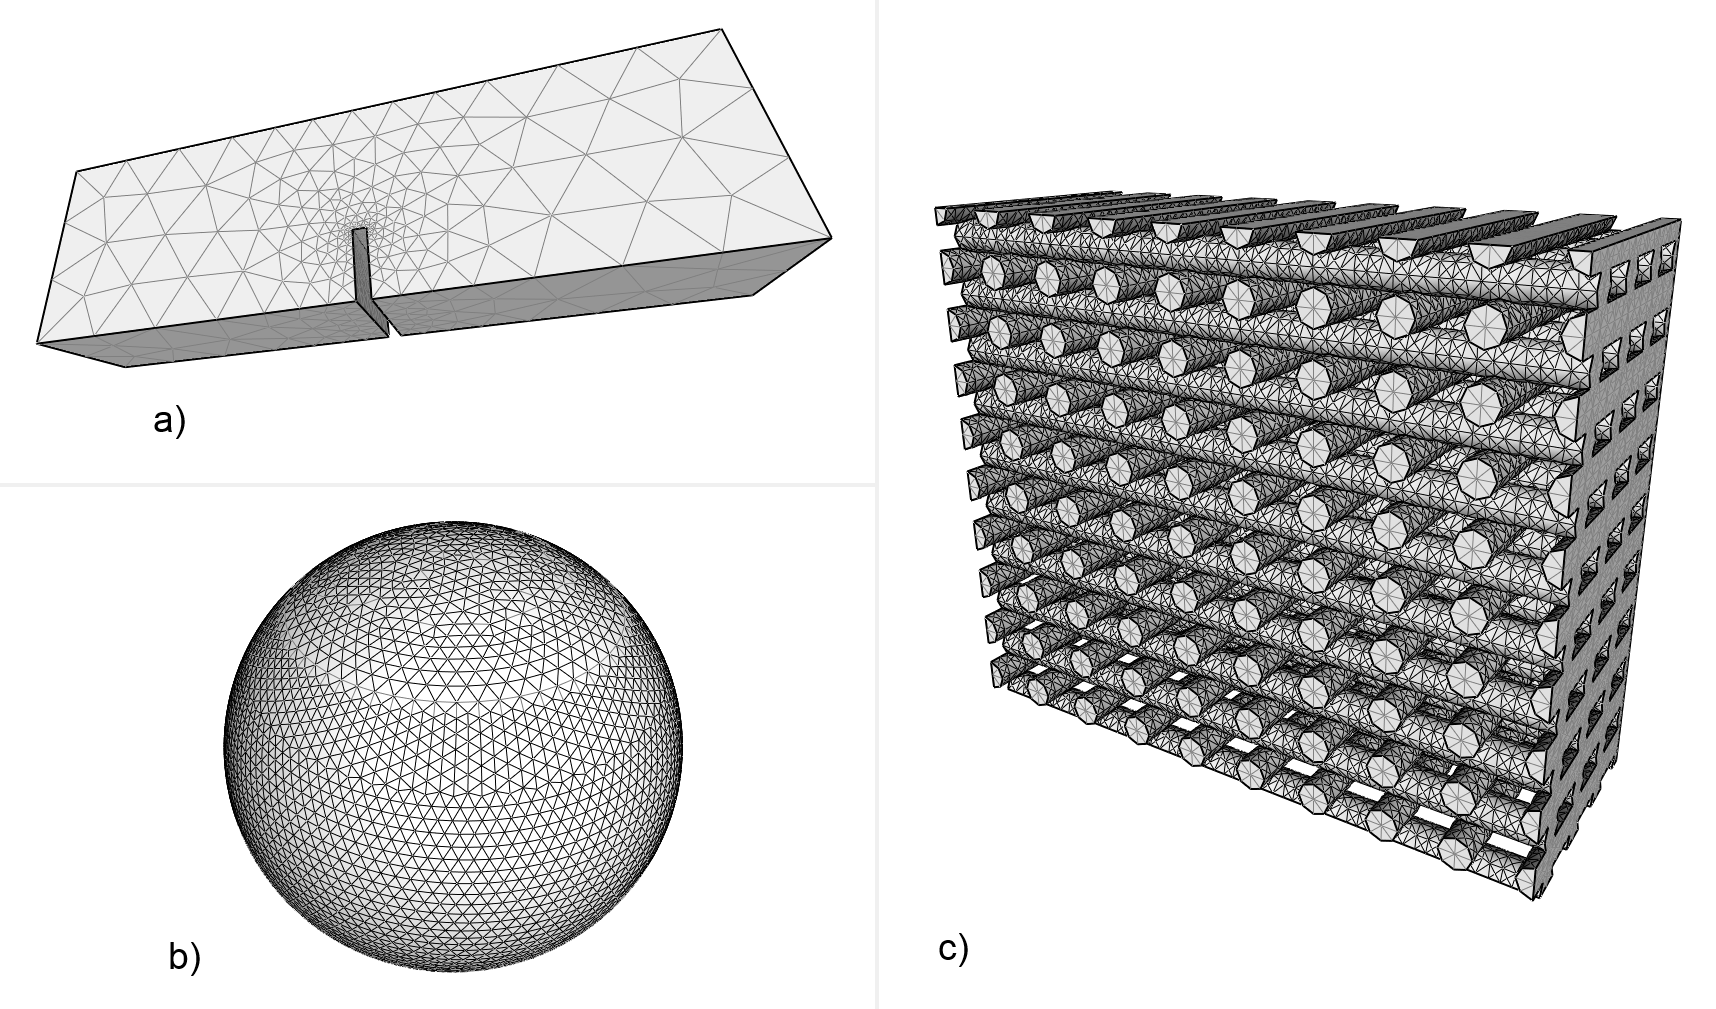
\includegraphics[width=\textwidth]{figures/chapter-mesh-visualization/figure8}
\decoRule
\caption[Meshes for benchmarks]{Visualizations of meshes used in benchmark. Three different densities of the Beam mesh were used to demonstrate the effects of mesh size. Meshes Sphere and Robo show effect of surface area/volume ratio. a) Beam. b) Sphere. c) Robo.}
\label{fig:benchmark-meshes}
\end{figure}

\begin{figure}[H]
\centering
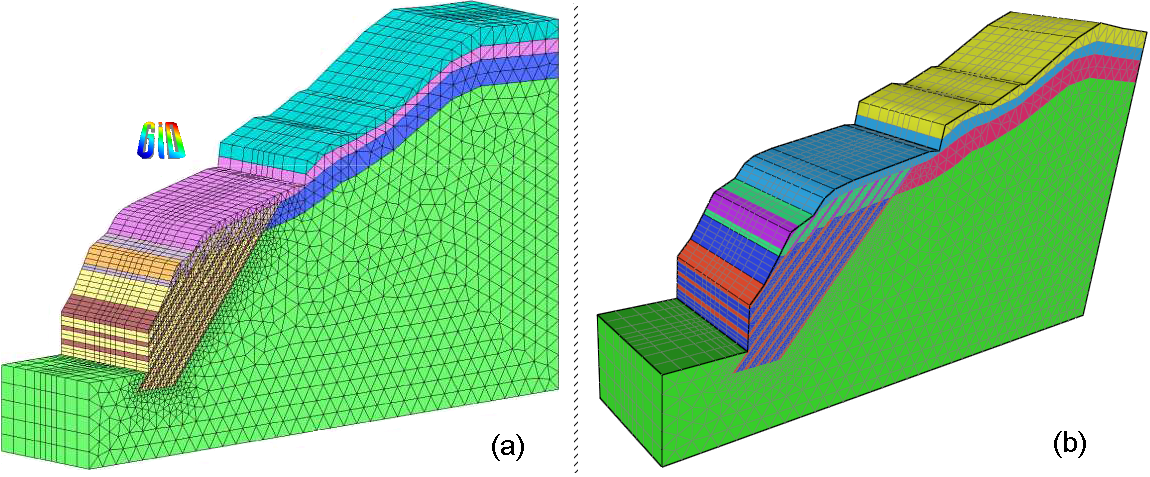
\includegraphics[width=\textwidth]{figures/chapter-mesh-visualization/figure9}
\decoRule
\caption[Visualization of significant edges]{Finding and visualization of significant edges. a) GiD postprocessor. b) The Mesh Editor.}
\label{fig:significant-edges}
\end{figure}

For benchmarking we used PC with Intel Core i7-2600 processor, 16 GB memory and NVidia GeForce GT 545 graphics card. The results support the fact, that more complex data structure is constructed to represent the mesh in our editor. The manipulation with the model is comfortable even for a very large data input. The program takes benefit of creating the sophisticated internal data structure that, on the contrary, causes longer initial loading time. However, the presented smart internal model representation allows selection of logically related groups of entities on the mesh surface without knowing the geometrical and topological connections from the modeller. The program is able to find automatically the significant edges where the geometry changes (shown in Figure \ref{fig:significant-edges}) and therefore simplify the process of selecting the entities. Moreover, individual elements can be easily removed so it is allowed to dig into the mesh and view the internal elements. The other editors, which were tested against the proposed editor, do not support those features. Besides that, the capability of unlimited view-point movement allows to fly through holes in the mesh and investigate the mesh from the inside.
\chapter{Approximation of FEA results by polynomial functions}
\label{chapter:approximation}

% TODO: odebrat prvni 2 vety, jsou nadbytecne a zrejme, uz o tom mluvim nekde v uvodu asi?
The method of approximation of output from the Finite element method is based on premise, that computer memory and performance are limited. Without some kind of simplification or compression no program can efficiently process large amount of data generated by extensive finite element analysis. This chapter contains description of a proposed method for approximation of results from the Finite element method, which are discrete values, by polynomial functions. The approximation method is also presented in \cite{Benes2016}.

%----------------------------------------------------------------------------------------
%	SECTION Idea
%----------------------------------------------------------------------------------------

\section{Idea}

The multigrid method \cite{XXX6-9} was the inspiration for this work. Multigrid method allows to solve partial differential equations using the hierarchy of domain discretizations. The main idea of multigrid method is to make the convergence of iterative method faster due to global corrections of error that is made from time to time on the coarser mesh. There are many variations of multigrid method. However, all of them need existence of mesh hierarchy that represents domain discretizations of different mesh sizes.

Basic steps of multigrid method are:

\begin{itemize}
    \item \textbf{Smoothing} -– The main goal of the smoothing phase is the high-frequency error reduction. It can be done e.g. by few iterations of the Gauss-Seidel method.
    \item \textbf{Restriction} -- Restriction of the residual from the finer to the coarser mesh.
    \item Solution of the coarse problem.
    \item \textbf{Prolongation} -- Interpolation and projection of the correction computed on the coarser mesh to the finer mesh.
\end{itemize}

The main problem with a mesh hierarchy is that often none is available. Only the finest mesh exists. The coarser meshes must be either generated directly by a mesh generator \cite{XXX-10, XXX-11} in the pre-processing phase or it must be created from the finer mesh. But generating coarser mesh from the finer one is very problematic or even impossible, because corresponding nodes between different levels should be preserved to be sure that multigrid method will work correctly without special modifications.

Therefore, it was decided to do visualization of the results from the finite element analysis on the fine mesh that is used for solution of FEM. Different methods of simplification and compression of the resulting data in space and time were developed and data were projected back to fine mesh. Results of the projection and comparison of methods are presented in this paper.

%----------------------------------------------------------------------------------------
%	SECTION Implementation
%----------------------------------------------------------------------------------------

\section{Implementation}

Even if the mesh hierarchy is generated, one of the obstacles for using the same multigrid techniques as are often used in the finite element analysis is that only one mesh hierarchy is available. That is sufficient for finite element solver, because this hierarchy is used to solve only one set of equations. However, in the post-processor it is necessary to display various kinds of data, such as temperature, displacements, stress, strain, etc. These quantities are scalars, vectors or tensors of second order. Components of vectors and tensors could be considered in post-processing as a scalar and therefore scalars will be dealt in the following text. Every scalar is represented in the finite element analysis by a set of discrete values computed in nodes or Gauss points, but in the strong formulation of a problem, it is a function. For graphical purposes, it is possible and often suitable to replace the set of discrete values by a continuous function. In the following text, the set of discrete values describing a scalar will be denoted as the discrete function or original function, but approximation of the discrete values for graphical purposes by continuous function will be called approximation function (shape functions used in FEM are not used here).

Approximation functions should be as simple as possible to be representable by a small set of parameters. Therefore, the domain of approximation function should respect the character of the discrete function. It can’t be the whole mesh, because one part of mesh could contain data replaceable by a simple linear function and other part could have much wilder character. It is therefore necessary to find alternative division of problem domain that will respect the shape of function in space and time better than the mesh hierarchy used in the multigrid method. Moreover, each quantity component must have its separately generated mesh hierarchy.

%----------------------------------------------------------------------------------------
%	SUB-SECTION Octree generation
%----------------------------------------------------------------------------------------

\subsection{Octree generation}

Domain space has to be divided into subdomains of the size which allows to replace discrete function with continuous, simpler, e.g. linear function that is easy to describe by fewer parameters. The goal is to automatically recognize areas in mesh, where the nature of function is smooth (the function is continuous together with the first derivatives and very coarse mesh can be used) and areas in which function rapidly changes its character (the first derivatives are large or the function is even discontinuous). These areas of interest become object of further subdivision, because for visualization purposes they need finer underlying mesh. For recursive division of 3D space the octree data structure is suitable (see Figure \ref{fig:octree-visualization}). The other spatial dividing data structures used in computer graphics were investigated, but octree seemed to be the best choice due to its hierarchical form and low average depth.

\begin{figure}[H]
\centering
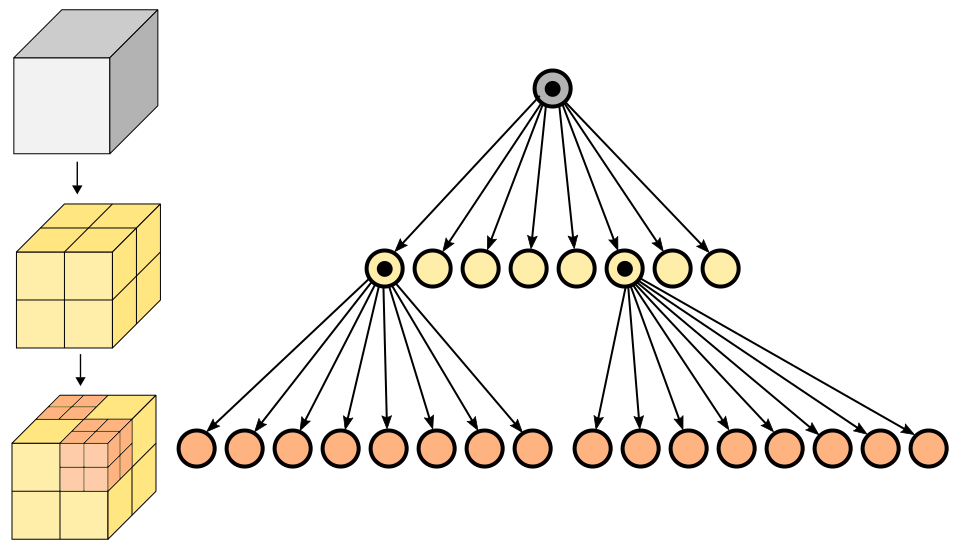
\includegraphics[width=\textwidth]{figures/chapter-approximation/figure1}
\decoRule
\caption[Octree visualization]{Octree visualization. Left: Recursive subdivision of a cube into octants. Right: The corresponding octree.}
\label{fig:octree-visualization}
\end{figure}

Basic overview of the decomposition and approximation procedure is in Listing \ref{alg:approximation}. At first whole mesh is inserted into one big cube -- octree root node. Then a condition that tells whether to divide current domain into eight subdomains is needed. Three conditions were designed. All have to be satisfied to proceed with decomposition.

\begin{enumerate}
    \item First condition specifies minimum number of finite element nodes to be represented by single octree cell. There are two reasons. Firstly, some specification of minimum number is necessary to compute approximation function, e.g. least square trilinear algorithm needs at least 8 values. Secondly, if the number is too small and the approximation function does not fit ideally, subdivision of the octree will be too subtle and memory consumption will easily exceed the case with no approximation applied at all.
    \item Second condition is based on maximal allowed relative error of chosen approximation function. Algorithm that replaces discrete data points with continuous approximation function also calculates relative error of the method. This number is then compared with some preset fixed value. According to the experiment results the most appropriate value of 1\% was chosen.
    \item Third condition describes maximum depth of octal tree. Each level of the tree exponentially increases memory consumption of data values stored in octree. Maximum depth is therefore artificially set to some acceptable value, e.g. 9. However, this depth should not be reached in common cases, it is ensured by condition 1.
\end{enumerate}

If all conditions are met, domain represented by the current octree node is divided into eight subdomains. Differences between original value of discrete function and value of approximation function in the same point are transferred to corresponding sub-nodes based on their location and whole process is recursively repeated in all octree sub-nodes. The difference $D_i$ of the $i$-th data value is defined by

\begin{equation}
D_i=V_i-\bar{V}_i, % or \overline ?
\end{equation}

where $V_i$ is the original function value in the $i$-th node and $\bar{V}_i$ is the value of approximation function in the same location as the $i$-th node.

Similar procedure -- passing residuals between mesh levels -- is applied in the multigrid method. Due to this approach the top levels of octree filter out main character of function (lower frequencies), bottom levels and leaves of the octree catch higher frequencies of function values.

%----------------------------------------------------------------------------------------
%	SUB-SECTION Approximation in space
%----------------------------------------------------------------------------------------

\subsection{Approximation in space}
\label{sec:approximation-in-space}

Discrete values within an octree cell are replaced by a continuous function which is as simple as possible and can be represented in memory by a few parameters. It is therefore necessary to find suitable type of function and in the case of polynomial functions also the order of the function. Compression algorithm has to be very fast. Compromise between low error and memory consumption must be found. For the sake of simplicity at the beginning of the work the relations between neighboring octree nodes were neglected. Nodal values in each octree cell are approximated separately.

The compression procedure requires the surface representation of the mesh to be already created. The element connectivity and nodal coordinates has to be present in memory and accessible in constant $\mathrm{O}(1)$ time. Efficient methods to create this surface representation are described in Appendix \ref{chapter:mesh-visualization} and also in \cite{XXX}.

The procedure is reading the FEM results divided to data sets from the external file and then processing the data sets one by one. By a data set is meant primarily the array of floating-point numbers corresponding to one component of one quantity, e.g. $x$ component of displacement vector, temperature (which is scalar) or one component of stress tensor. Each floating-point number is the value of the quantity in single time step corresponding to one node or gauss-point. Whole array is loaded from file into computer memory, its values are distributed into growing octree and the approximation is calculated and saved in corresponding octree cells. After that the original data are deleted and algorithm continues with the next data component.

Compression has to be made on-the-fly during loading of data from the file to the memory between each data component. Starting compression after all results has been loaded to the memory would not make sense, because the main purpose of the compression step is to save overall memory consumption of the post-processor. Therefore, the format of data should ideally be designed in the way that each data component is separated in single data file or at least in one isolated data block in the file not mixed with other data. No particular order of data components is required. However, data formats used by common finite element software packages are usually designed in the way that the components of each quantity are grouped together. We rely mainly on GiD postprocess file format (\file{.res}) described in detail in \cite{XXX-12} where data are divided to blocks according to physical quantity and time step. Each block is the list of value tuples introduced by a node number (or element number in case of values in gauss-points), e.g. $x$, $y$ and $z$ component triplet for displacement vector in node $42$ in time step $3.0$. To avoid multiple passes through the data file the value tuples are cached and processed right after reading the whole data block.

\begin{lstlisting}[caption=Core of aproximation procedure,label=alg:approximation]
function OctreeInternalNode.InsertDataValues(dataValues, dataComponentId, depth, approximationMethod)
{
  // find approximation function and save it in current octree node
  approximation = ComputeApproximation(dataValues, dataComponentId, approximationMethod)
  DataCatalog[dataComponentId] = approximation
  // if condition #2 is met, propagate values to child nodes
  if (approximation.MaxRelativeError > MIN_RELATIVE_ERROR_TO_EXPAND)
  {
    // split residual values to octants based on data point positions
    foreach (dataValue in dataValues)
    {
      // calculate residual and distribute to octants according to position
      position = mesh.Nodes[dataValue.NodeId].Position
      residual = dataValue.Value - approximation.GetValueAt(position)
      octantIndex = getIndexOfOctantOnPosition(position)
      residuals[octantIndex].Add(new DataValue(residual, dataValue.NodeId))
    }
    foreach (octantIndex in range 1..8)
    {
      // if condition #1 is met, algorithm is recursively called on child octree node
      if (residuals[octantIndex].Count > max(MIN_LEAF_DATA_POINTS_COUNT, approximationMethod.MinNumberOfDataPoints))
      {
        // recursive call to InsertDataValues, if children[octantIndex] is LeafNode, than recursion is stopped
        children[octantIndex].InsertDataValues(residuals[octantIndex], dataComponentId, depth + 1, approximationMethod)
        // if child node is leaf, find out if expansion is needed
        if (children[octantIndex] is LeafNode)
        {
          // if condition #3 is met, algorithm can continue with octree node expansion
          if (depth < MAX_OCTREE_DEPTH - 1)
          {
            // if condition #2 is met, expand leaf node
            if (children[octantIndex].DataCatalog[dataComponentId].MaxRelativeError > MIN_RELATIVE_ERROR_TO_EXPAND)
            {
              children[octantIndex] = new OctreeInternalNode(children[octantIndex].LowerBounds, children[octantIndex].UpperBounds)
              children[octantIndex].InsertDataValues(residuals[octantIndex], dataComponentId, depth + 1, approximationMethod)
            }
          }
        }
      }
    }
  }
}

function OctreeLeafNode.InsertDataValues(dataValues, dataComponentId, depth, approximationMethod)
{
  // find approximation function and save it in current octree node
  DataCatalog[dataComponentId] = ComputeApproximation(dataValues, dataComponentId, approximationMethod)
}

function ComputeApproximation(dataValues, dataComponentId, approximationMethod)
{
  switch (approximationMethod)
  {
    case TrilinearInterpolation:
      approximation = DoLeastSquaresTrilinearInterpolation(dataValues)
    ...
  }
  // compute absolute error
  maxError = 0;
  foreach (dataValue in dataValues)
  {
    position = mesh.Nodes[dataValue.NodeId].Position
    error = dataValue.Value - approximation.GetValueAt(position)
    maxError = Max(maxError, Math.Abs(error));
  }
  approximation.MaxError = maxError;
  approximation.MaxRelativeError = maxError / GlobalDataRange[dataComponentId]
  return approximation
}    
\end{lstlisting}

After loading a data block, compression is started. Listing \ref{alg:approximation} contains pseudo-code of recursive procedure that is the core of the compression algorithm. Figure \ref{fig:octree-generation} contains overview of this algorithm in form of UML Activity diagram. The input is an array of nodal values in one component of one field defined on the mesh in single time step. In case of data stored in gauss-points the values has to be at first extrapolated to nodes using natural coordinates supplied in the data file. Nodal data are then passed as an input parameter \code{dataValues} to the function \code{InsertDataValues} that is called upon the octree root node which represents one big cube that surrounds the whole mesh. Each \code{dataValue} object is a structure consisting of floating-point number Value and integer \code{NodeId} that represents a key to the table of nodes in global mesh object. \code{InsertDataValues} is pure virtual function declared in abstract base class \code{OctreeNode} and its implementation differs in derived classes. Its implementation in \code{OctreeLeafNode} is straightforward and so follows description of its implementation in class \code{OctreeInternalNode}. Simplified class diagram of the key types involved in Listing \ref{alg:approximation} is shown in Figure \ref{fig:octree-class-diagram}.

\begin{figure}[H]
\centering
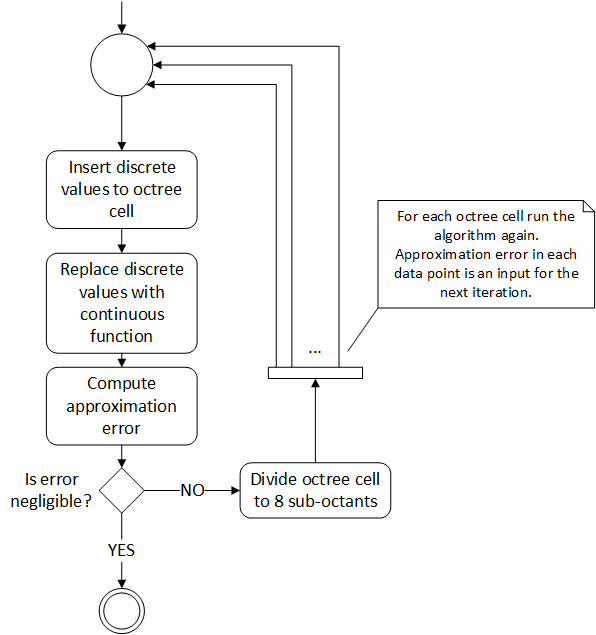
\includegraphics[width=\textwidth]{figures/chapter-approximation/figure2}
\decoRule
\caption[Octree generation]{Octree generation algorithm in form of activity diagram.}
\label{fig:octree-generation}
\end{figure}

\begin{figure}[H]
\centering
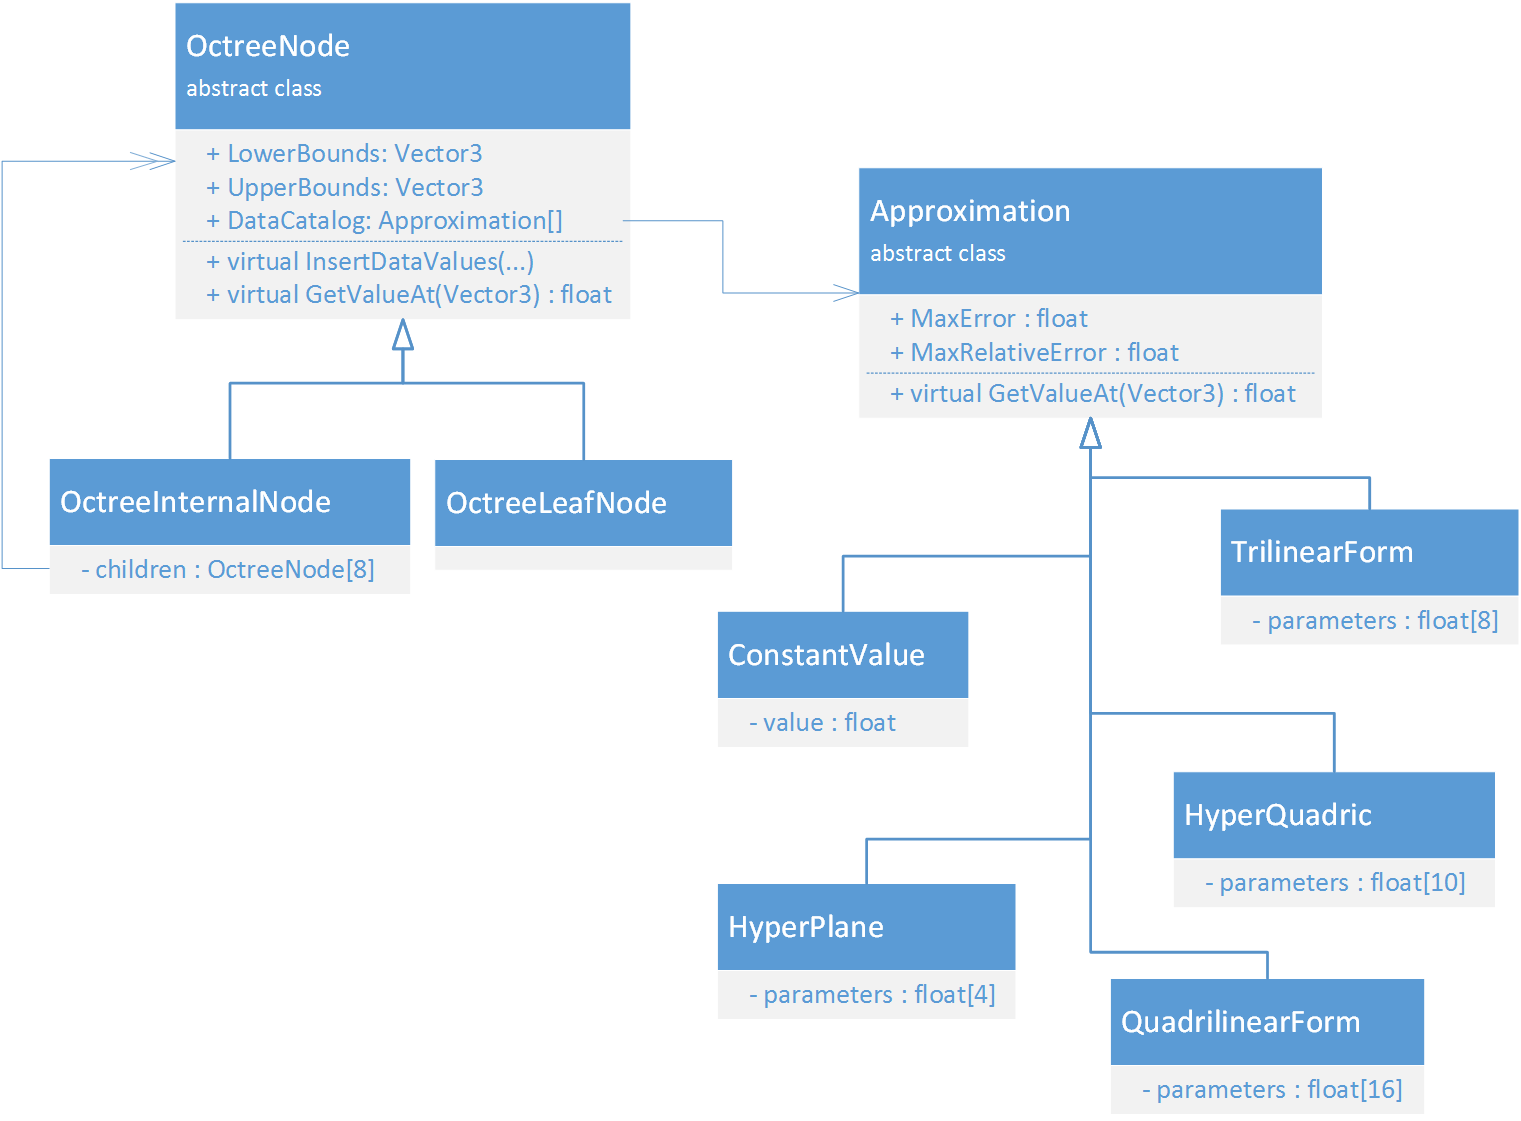
\includegraphics[width=\textwidth]{figures/chapter-approximation/figure3}
\decoRule
\caption[Diagram of octree generation classes]{Class diagram of types involved in octree generation algorithm.}
\label{fig:octree-class-diagram}
\end{figure}

At first the algorithm computes parameters of continuous approximation function of discrete data values provided (variable \code{approximation}). In case of trilinear interpolation it uses least square method to calculate 8 parameters of a polynomial regression model and stores them in \code{DataCatalog} table which is a property of each octree node. Then the maximal relative approximation error is computed.

Approximation function for data values in the octree cell is assessed with the help of several metrics. First, absolute approximation error, which is the difference between the original nodal value and the value of approximation function, is evaluated in all nodes. Then, relative approximation error is obtained by dividing the absolute approximation error by global range of values (difference between global maximum and global minimum of original nodal values). The maximum relative approximation error in an octree cell is one of three parameters (see condition 2 above) that are used by the algorithm to decide whether to proceed with further subdivision of the octree cell. These three parameters control the overall quality of approximation, memory consumption and performance and need to be fine-tuned during testing on real-world data.

If the maximal approximation error is too high, the algorithm continues, calculates approximation error in each node and stores it in table residuals in relevant octant according to its position in current octree cell. \code{residuals} is a table of data value arrays and it is a local variable that will be disposed after each call to function \code{InsertDataValues} finishes. Algorithm then iterates over all child octants and checks for number of residuals assigned to them. If condition 1 stated above holds, algorithm is recursively called upon each child octree cell. If the octree cell is a leaf node, recursion is stopped and algorithm determines whether it should split current leaf octree cell into 8 sub-segments by checking conditions 2 and 3. In other words, if the current octree branch is not deep enough and maximal residual belonging to current child octree cell is higher than designated epsilon value, then this leaf cell is replaced with internal cell and function \code{InsertDataValues} is called upon this new \code{OctreeInternalNode} object. Residuals located in current octant are passed as an input to this function.

This continues until approximation of current data component is good enough in all octree cells.  When the algorithm finishes, original discrete data can be deleted, because the created octree structure with approximation functions in its nodes is all that is needed to reconstruct the original data. Then the algorithm can proceed with reading and processing next data set. Note that these operations are to a considerable extent independent and processing of data sets can be parallelized. However, if the same octree data structure is reused for multiple data sets, then the access to \code{DataCatalog} and octree node expansion has to be synchronized using standard locking mechanisms.

Also note that passing residuals of approximation instead of original data between octree levels is important, because it allows to describe the main character of function (lower frequencies) on top levels and details (high-frequency changes) on bottom levels of the octree. This design is inspired by the Multigrid method basic principles.

%----------------------------------------------------------------------------------------
%	SUB-SUB-SECTION Approximation functions
%----------------------------------------------------------------------------------------

\subsubsection{Approximation functions}

Various approximation functions were investigated and tested. Besides polynomial functions also Discrete cosine transform \cite{XXX-13} and Wavelet transform \cite{XXX-14} were considered. Since the data compression algorithm has to be very fast, simple polynomial approximation functions were preferred. They are summarized below:

\begin{itemize}
  \item \textbf{Mean value} -- A single value (average value) replaces the set of discrete values. Arithmetic mean was used during testing because it is fast to compute unlike the median. Also, it takes into account whole spectrum of values in contrast of the mode value that is the value that occurs most often in the collection. It is suitable in statistics where the measurement errors have to be excluded. However, in the case of the results from the FEM the user wants to see extremes in data and these outlying results should be rather highlighted instead of truncated. That is the reason why is neither the arithmetic mean nor other statistically estimated mean value suitable for this purpose. Mean value approximation diagram is depicted in Figure \ref{fig:mean-value-approx}.

  \begin{figure}[H]
  \centering
  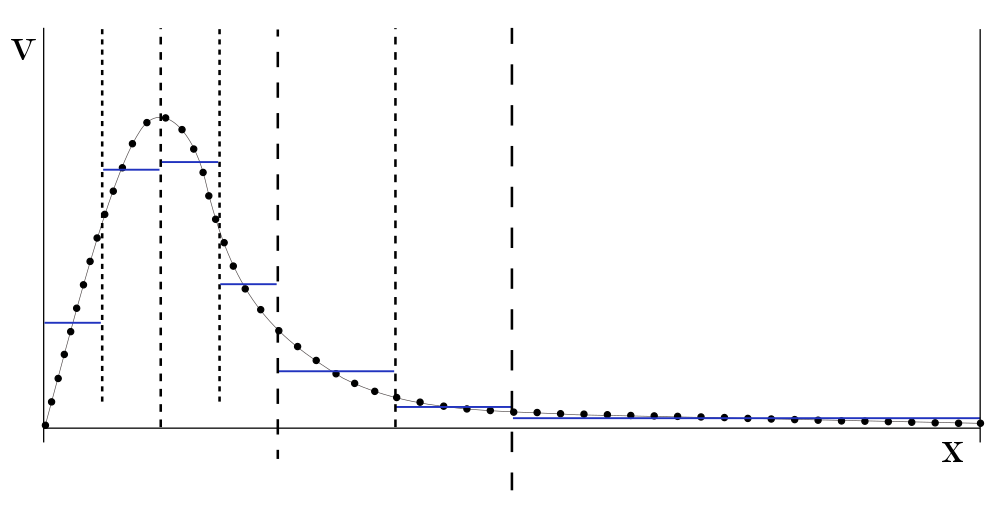
\includegraphics[width=\textwidth]{figures/chapter-approximation/figure4}
  \decoRule
  \caption[Mean value approximation diagram]{Mean value approximation diagram. Dashed lines denote octree division process. Shorter the line the deeper subdivision represents. Mean value is not suitable because of high errors and discontinuities between approximation cells. $v$ stands for function value and $x$ for spatial dimension.}
  \label{fig:mean-value-approx}
  \end{figure}

  \item \textbf{Regression} -- Finds a polynomial that models relationship between a scalar dependent variable and one or more explanatory (independent) variables. In three-dimensional problem there are three independent variables. Polynomial regression models are often fitted using the least squares method. The implementation used in this work is based on solving linear system of equations using LU decomposition. Key thing is that the size of the system does not depend on the number of data values, but on the number of approximation function parameters. Therefore, the algorithm has linear computational complexity and scales well. Several polynomials were tested. In the functions below $x$, $y$, $z$ are spatial coordinates, $c_i$ are parameters which determine the shape of the polynomial and $v$ is the function value.

  \begin{itemize}
    \item \textbf{Linear} -- Hyperplane, only four parameters per octree cell. Value $v$ in the point with coordinates $x$, $y$, $z$ is computed using linear interpolation function in the form
    
    \begin{equation}
    v=c_{1}x + c_{2}y + c_{3}z + c_{4}.
    \end{equation}
    
    Figure \ref{fig:octree-creation} contains example of creation of octree node hierarchy driven by this function.
    
    \item \textbf{Quadratic} -- Parametric shape models known as Hyperquadrics. They have too many parameters per cell (10) and are not suitable to capture continuity between octree cells. Value v in the point with coordinates $x$, $y$, $z$ is computed using quadratic interpolation function in the form

    \begin{equation}
      v=c_{1}x^2 + c_{2}y^2 + c_{3}z^2 + c_{4}xy + c_{5}xz + c_{6}yz + c_{7}x + c_{8}y + c_{9}z + c_{10}.
    \end{equation}

    \item \textbf{Trilinear} -- 8 parameters, the best compromise, consistent with neighboring octree cells, almost “seamless” transitions between octree cells. Also used in the FEM. Value $v$ in the point with coordinate $x$, $y$, $z$ is computed using trilinear interpolation function in the form
    
    \begin{equation}
      v=c_{1}xyz + c_{2}xy + c_{3}xz + c_{4}yz + c_{5}x + c_{6}y + c_{7}z + c_{8}.
    \end{equation}

    The least squares method is applied to find parameters $c_{1},...,c_{8}$. The problem is solved by minimizing the sum of squared residuals $G$ of the linear regression model

    \begin{equation}
      G = \sum_{i=1}^{N}(v_i - (c_{1}x_{i}y_{i}z_{i} + c_{2}x_{i}y_{i} + c_{3}x_{i}z_{i} + c_{4}y_{i}z_{i} + c_{5}x_{i} + c_{6}y_{i} + c_{7}z_{i} + c_{8}))^2,
    \end{equation}
    
    where $N$ is number of values which are interpolated. When the parameters of interpolation are known, value in any point of the approximated volume can be found simply by providing $x$, $y$, and $z$ coordinates of the point in the equation.
    
    \item \textbf{Tri-quadratic} -- Too many describing parameters with no significant benefit over trilinear form.
    
    \item \textbf{Quadrilinear form} -- Generalized trilinear form, extended by temporal dimension, only theoretical option, not implemented.
    

  \end{itemize}

\end{itemize}

\begin{figure}[H]
\centering
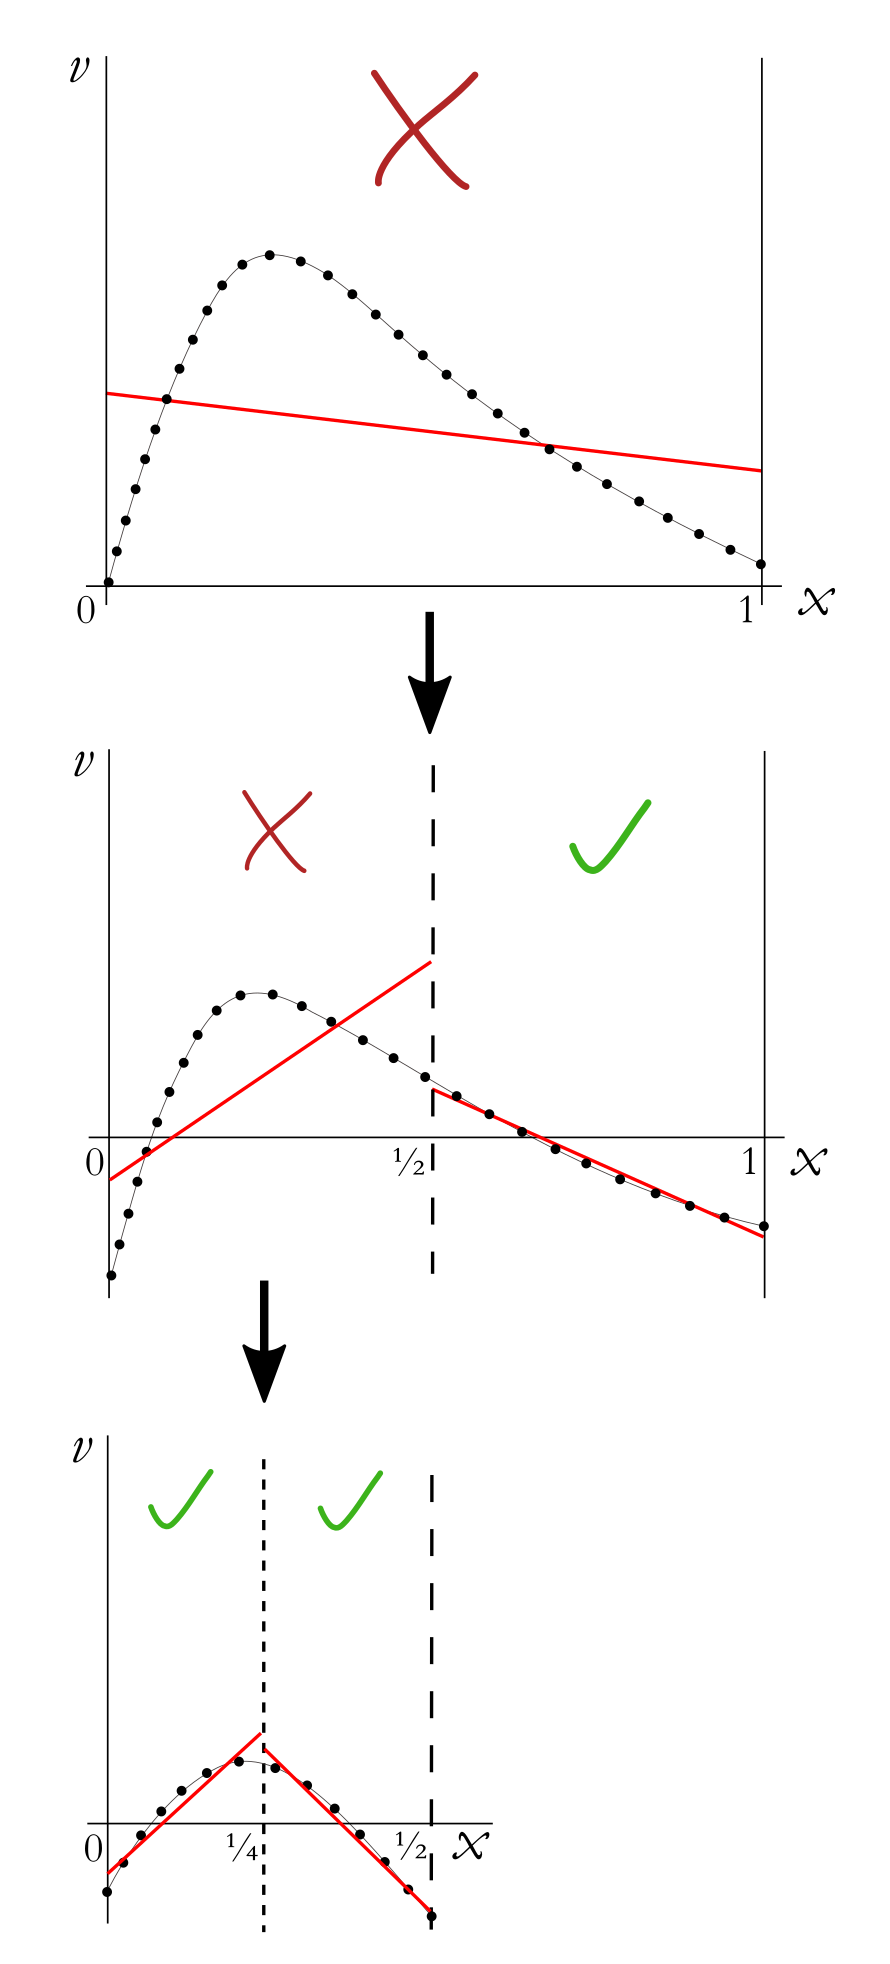
\includegraphics[width=0.5\textwidth]{figures/chapter-approximation/figure5}
\decoRule
\caption[Octree creation]{Octree creation example based on linear approximation error.}
\label{fig:octree-creation}
\end{figure}

\begin{figure}[H]
\centering
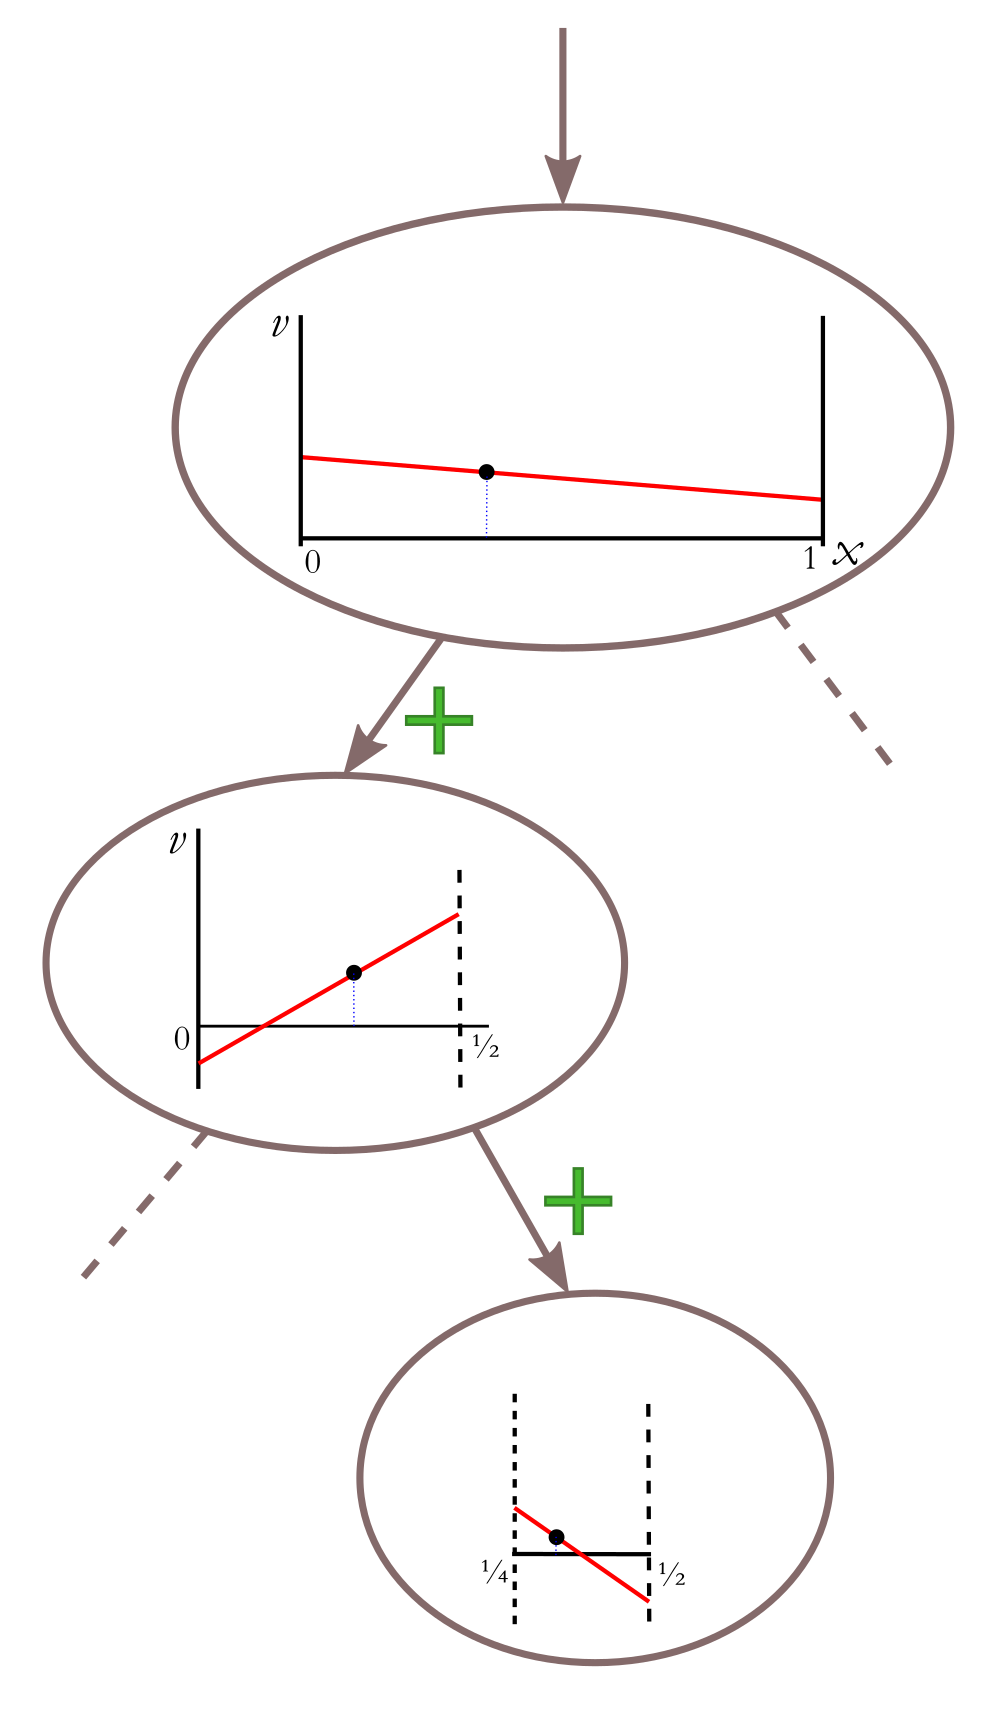
\includegraphics[width=0.5\textwidth]{figures/chapter-approximation/figure6}
\decoRule
\caption[Nodal value computation]{Nodal value computation diagram.}
\label{fig:nodal-value-computation}
\end{figure}

Figure \ref{fig:nodal-value-computation} depicts computation of nodal value via traversing octree from the root to the leaves and simultaneously summing up approximation errors. Root node of the octree contains all data components in all time steps where data value of an arbitrary element node can be computed. If an approximation is not sufficiently accurate in current octree node, correction can be made with the help of data stored in lower levels of the octree and summing up corrections together with initial value to compute final value for the node.

%----------------------------------------------------------------------------------------
%	SUB-SUB-SECTION Results
%----------------------------------------------------------------------------------------

\subsubsection{Results}

The benchmark is designed to compare maximal relative approximation error, average error and compression ratio when using different approximation methods. Two test data sets were chosen (Figure \ref{fig:reactor-vessel-displacements} and Figure \ref{fig:reactor-containment-displacements}), both contain displacement vector values with three components ($u$, $v$ and $w$) and about 30 time steps. Maximal relative approximation error is the highest relative error of an approximation method in single element node across all data components and time steps. Average error is a weighted sum of approximation errors in all nodes and data components divided by the number of these approximations. Compression ratio is memory consumption of the proposed data representation divided by memory consumption of original post-processor that does not use any data approximation techniques. Results are summarized in Table \ref{tab:reactor-vessel-results} and Table \ref{tab:reactor-containment-results}. The mesh topology and result data sets that were used in this benchmark can be found at \cite{XXX-15}.  These files can be opened for reference in program GiD.

\begin{figure}[H]
\centering
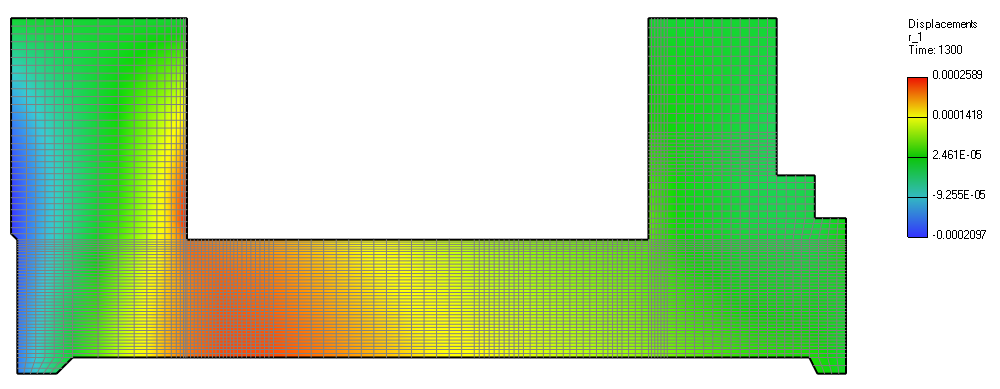
\includegraphics[width=\textwidth]{figures/chapter-approximation/figure7}
\decoRule
\caption[Reactor vessel 2D]{Reactor vessel 2D. Displacements visualization.}
\label{fig:reactor-vessel-displacements}
\end{figure}

\begin{table}[H]
\caption[Approximated results of reactor vessel 2D simulation]{Reactor vessel 2D. Spatial octree approximation results.}
\label{tab:reactor-vessel-results}
\centering
\begin{tabular}{| l | r | r | r |}
\hline
\tabhead{ } & \tabhead{Max error [\%]} & \tabhead{Average error [\%]} & \tabhead{Compression ratio [\%]} \\
\hline
Mean value & 75.28 & 0.6268 & 55.3\\
Linear regression & 44.23 & 0.1842 & 17.7\\
Trilinear regression & 81.27 & 0.1751 & 16.9\\
\hline
\end{tabular}
\end{table}

\begin{figure}[H]
\centering
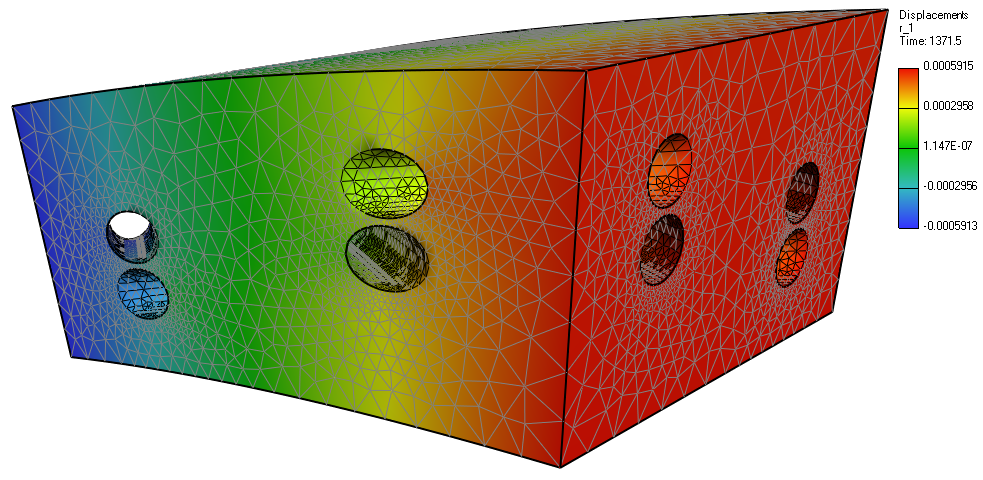
\includegraphics[width=\textwidth]{figures/chapter-approximation/figure8}
\decoRule
\caption[Segment of reactor containment]{Segment of reactor containment. Displacements visualization.}
\label{fig:reactor-containment-displacements}
\end{figure}

\begin{table}[H]
\caption[Approximated results of reactor containment simulation]{Segment of reactor containment. Spatial octree approximation results.}
\label{tab:reactor-containment-results}
\centering
\begin{tabular}{| l | r | r | r |}
\hline
\tabhead{ } & \tabhead{Max error [\%]} & \tabhead{Average error [\%]} & \tabhead{Compression ratio [\%]} \\
\hline
Mean value & 38.62 & 1.667 & 63.1\\
Linear regression & 32.9 & 0.305 & 59.4\\
Trilinear regression & 89.46 & 0.2237 & 56\\
\hline
\end{tabular}
\end{table}

\begin{figure}[H]
\centering
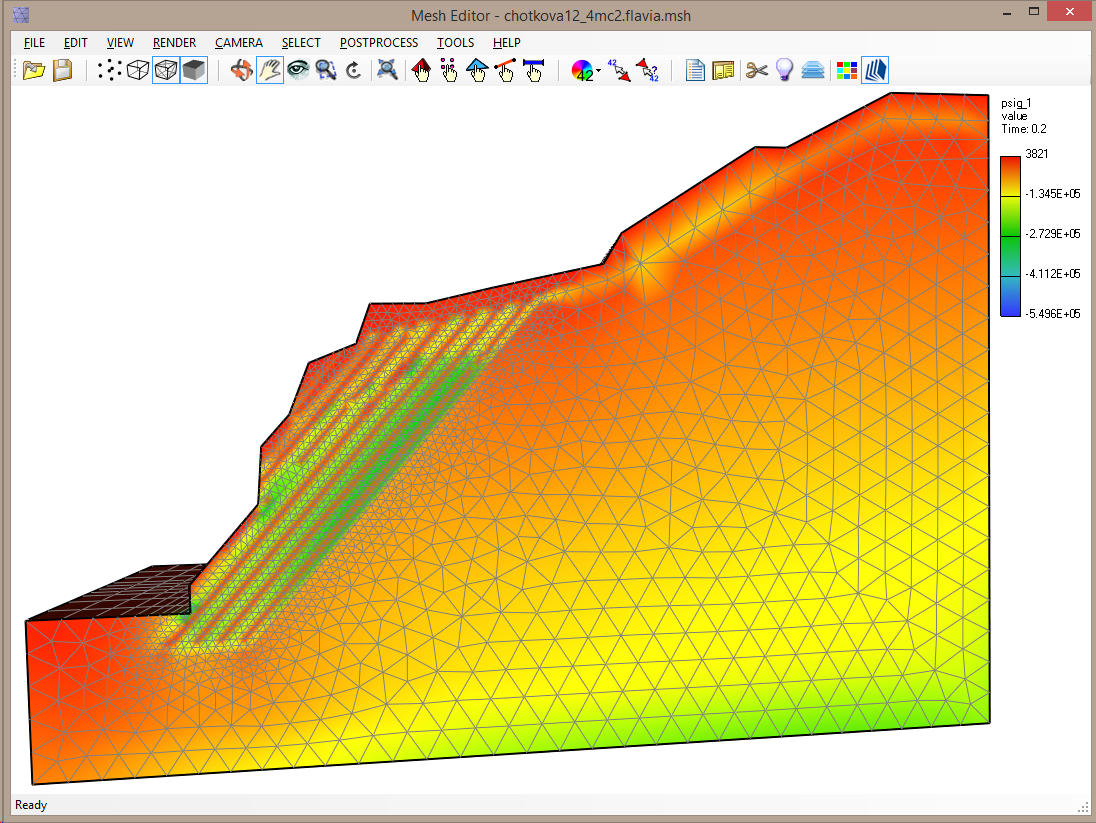
\includegraphics[width=\textwidth]{figures/chapter-approximation/figure9}
\decoRule
\caption[Geological layers simulation results]{Geological layers simulation results. Exact data values, no approximation applied.}
\label{fig:geological-layers-exact}
\end{figure}

\begin{figure}[H]
\centering
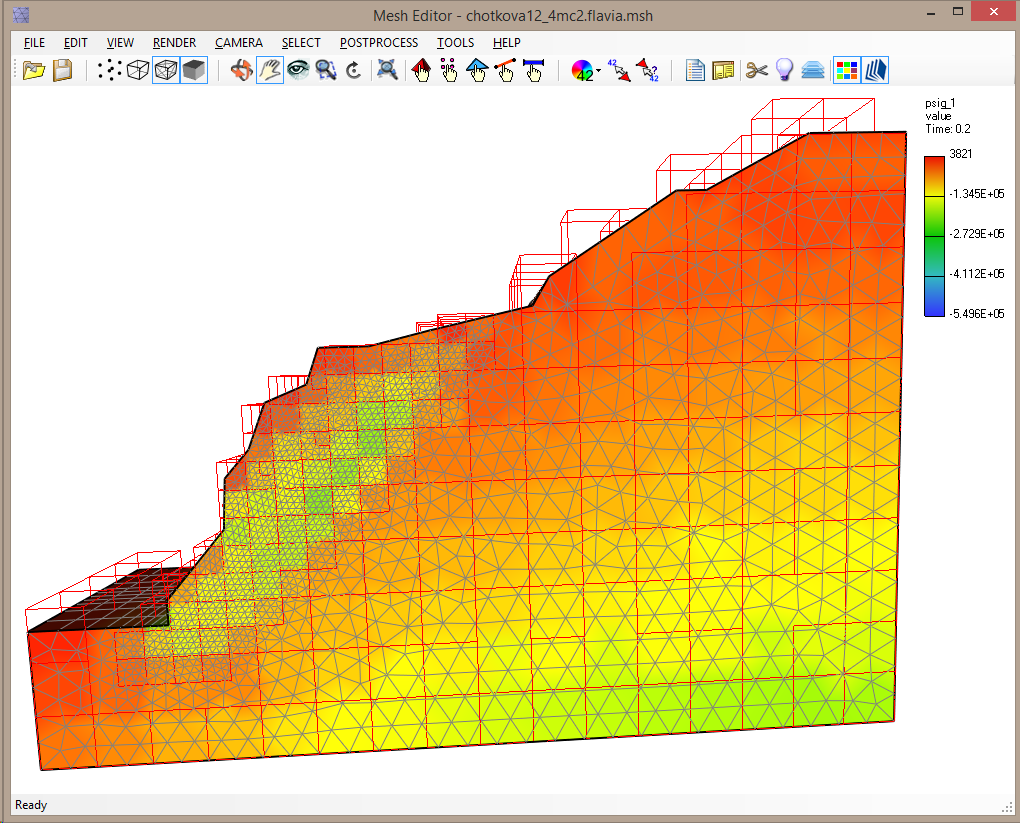
\includegraphics[width=\textwidth]{figures/chapter-approximation/figure10}
\decoRule
\caption[Mean value approximation of geological layers simulation results]{Geological layers simulation results. Mean value approximation of data values. Nodes in each cell have constant approximated value. High average error of an approximation. High memory consumption due to high average depth of the octree. Non-smooth transition between cells.}
\label{fig:geological-layers-mean}
\end{figure}

\begin{figure}[H]
\centering
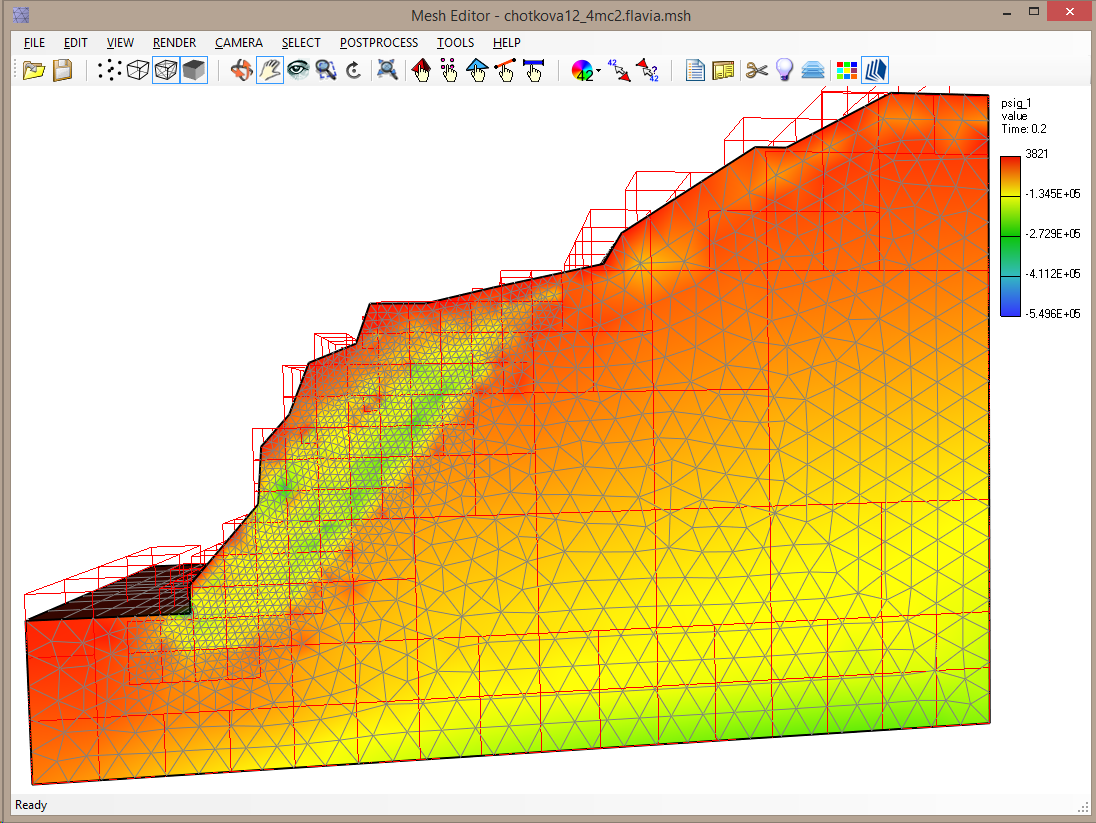
\includegraphics[width=\textwidth]{figures/chapter-approximation/figure11}
\decoRule
\caption[Trilinear approximation of geological layers simulation results]{Geological layers simulation results. Trilinear approximation of data values. Seamless transition between cells. Low depth of the octree in smooth areas. Can't capture high frequent changes in data which is common disadvantage of all lossy compressions.}
\label{fig:geological-layers-trilinear}
\end{figure}

Figure \ref{fig:geological-layers-exact} contains visualization of the exact data values whereas Figure \ref{fig:geological-layers-mean} and Figure \ref{fig:geological-layers-trilinear} contains visualization of approximation of the same data series but for different types of approximation functions to highlight the imperfections of the approximation algorithm. The red lines represent the octree cells.


%----------------------------------------------------------------------------------------
%	SUB-SECTION Approximation in time
%----------------------------------------------------------------------------------------

\subsection{Approximation in time}

Additional data compression can be gained by focusing on temporal dimension of function values. Memory allocation can be lowered by eliminating unimportant time steps. To achieve that, it is necessary to find those time steps, in which function values are steady or are changing linearly and can be therefore interpolated from other time steps.

Figure \ref{fig:interpolation-in-time} illustrates the idea of interpolation in time. Intermediate time steps can be interpolated from the key time steps if they have similar shape -- they are \textit{nearly} linear combinations of each other and therefore data in redundant time steps can be disposed. The decision whether to dispose time step or not is based on difference of two functions compared to experimentally designated threshold value. Mathematical background of this procedure is described later in this section.

\begin{figure}[H]
\centering
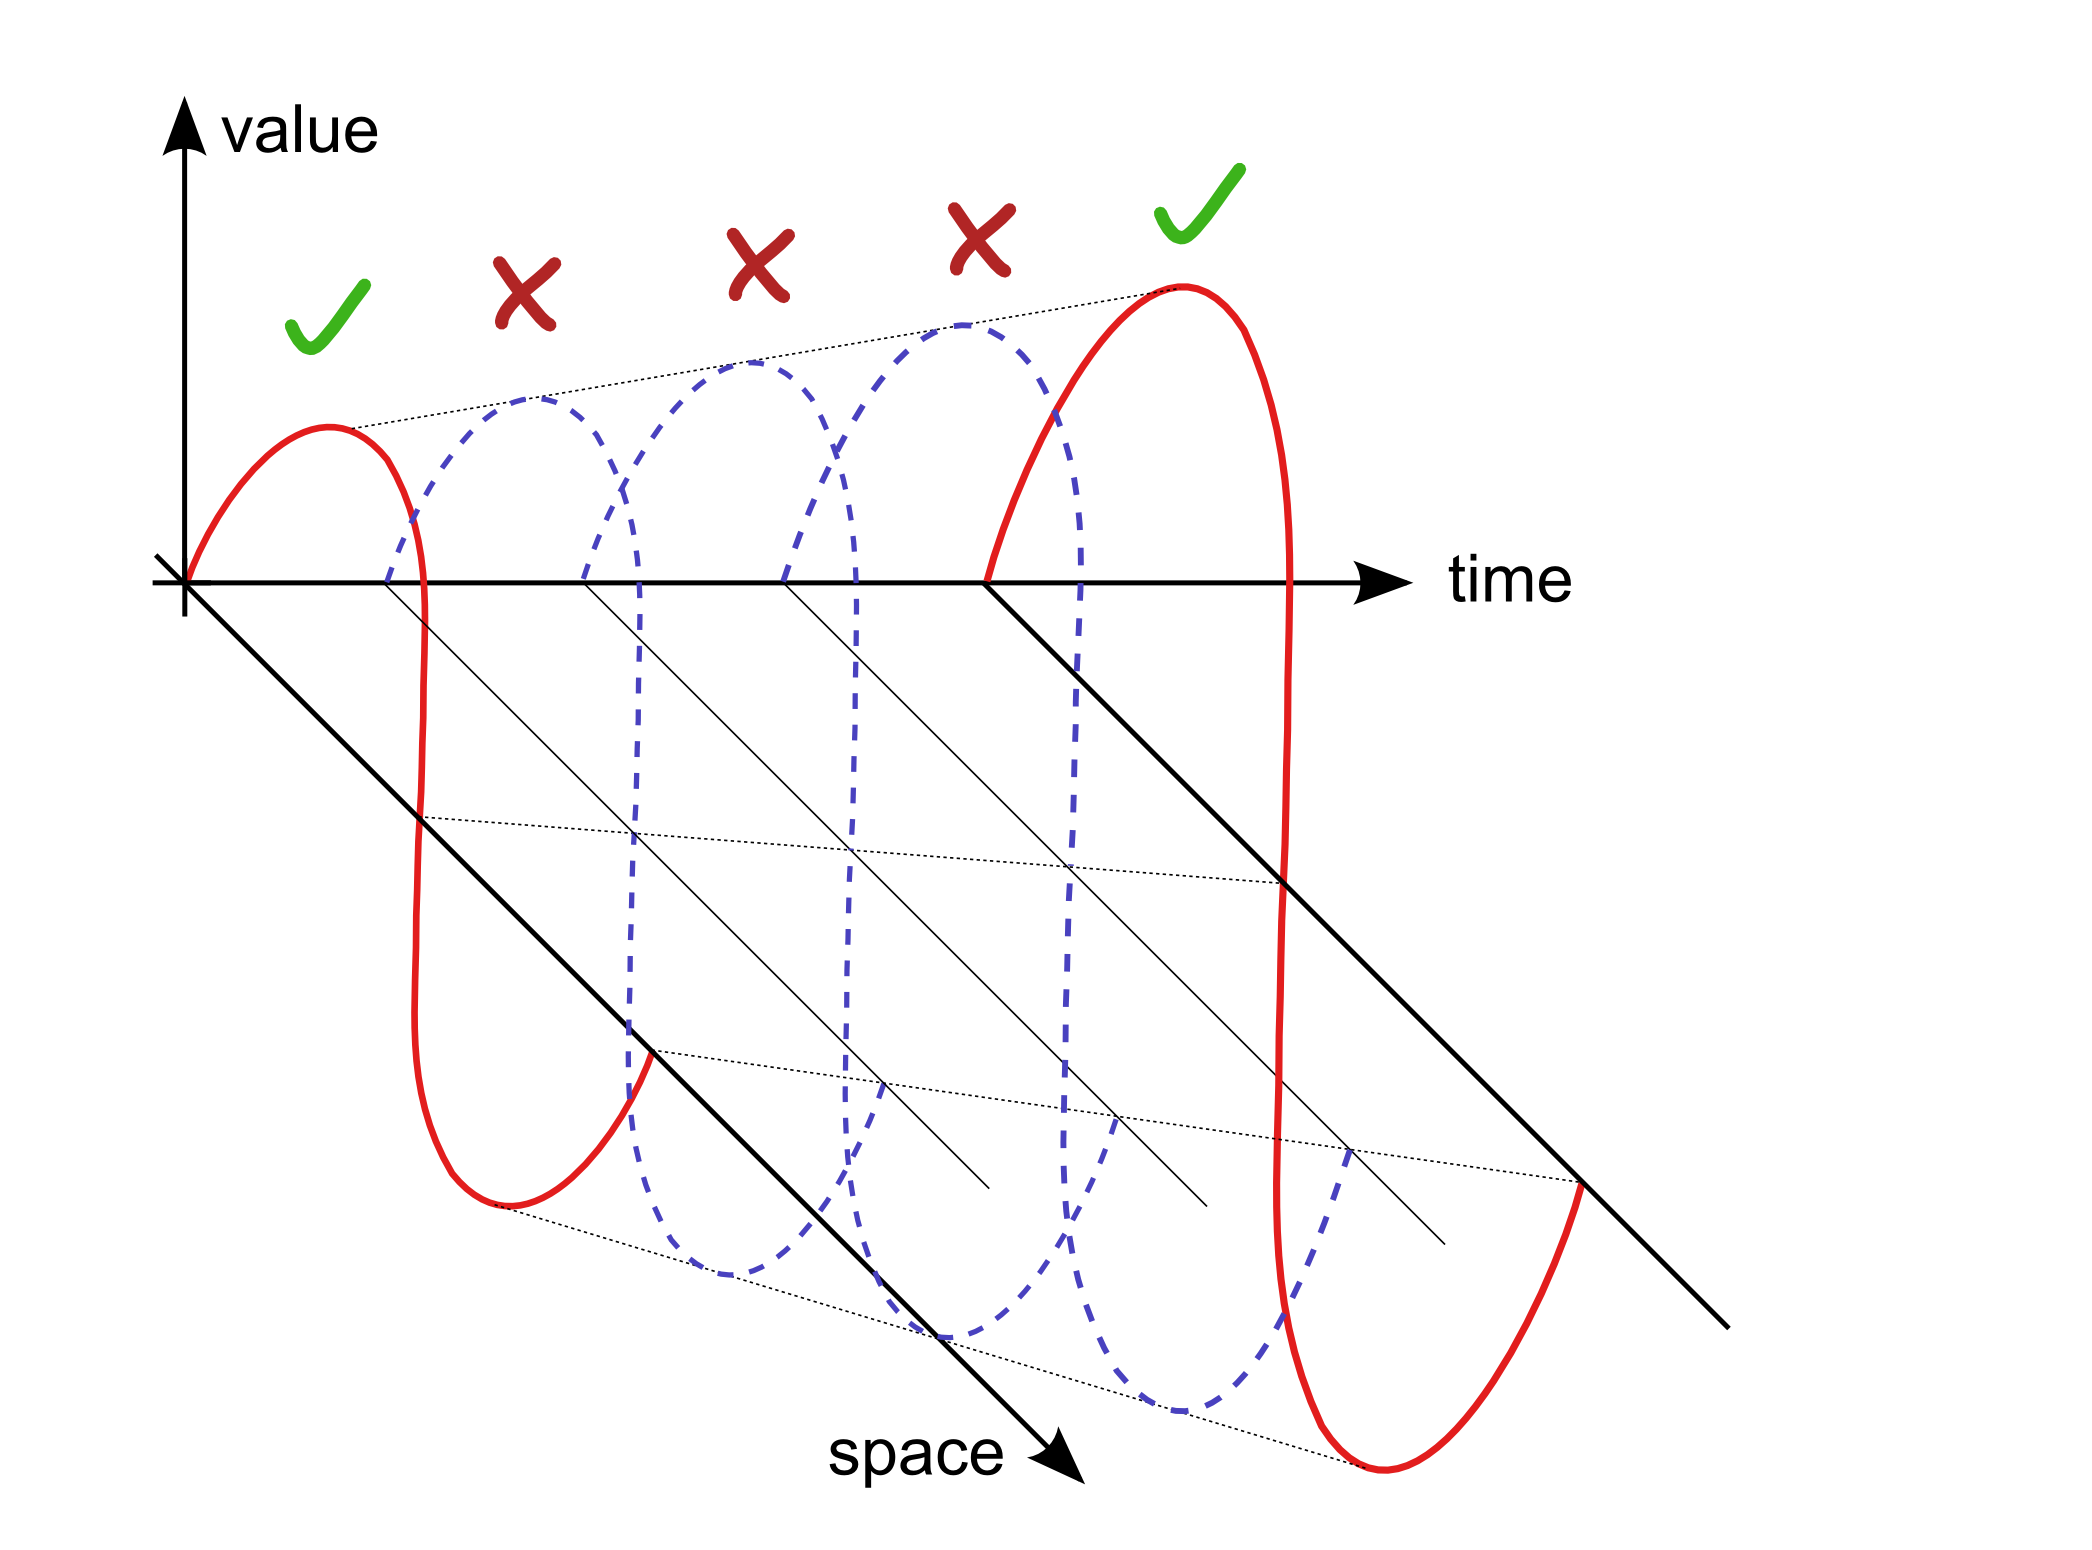
\includegraphics[width=\textwidth]{figures/chapter-approximation/figure12}
\decoRule
\caption[Interpolation in time diagram]{Interpolation in time. Intermediate time steps (blue) can be interpolated from the key time steps (red) if they have similar shape.}
\label{fig:interpolation-in-time}
\end{figure}

Several options to store temporal data were considered.

\begin{itemize}
  \item Sequence of octrees. Each one for single time step.
  \item 4D tree. Extension of octal tree on temporal dimension. Each internal node has 16 children.
  \item Single ordinary octree containing data approximations with time component. Extending the approximation functions by temporal dimension, e.g. quadrilinear form instead of trilinear form.
  \item Combination of octree for spatial decomposition and binary tree for temporal dimension division.
\end{itemize}

Octree for each time frame of an animation is memory inefficient as well as 4D tree \cite{XXX-16}. 4D approximation functions have many parameters and also can’t capture intricate evolution of function in time. Therefore, different solution was suggested -- single octree representing spatial decomposition that is formed by merging sequence of octrees from all time steps. However, the sequence of octrees is just a virtual term. Algorithm 1 treats all data component from all time steps the same and when it finishes its job, only single octree is left with data approximation object for various data component and time steps stored in data catalog in each octree node independent to each other. By merging it is meant the unifying all time steps of a single data component in each octree node into single data sequence object that can be then a subject of the time compression algorithm. This process of merging virtual octrees for each time step into single ``time-tree'' is illustrated in Figure \ref{fig:unifying-time-steps}. Notice that the octree for each time step can have different structure and depth, because in each time step the original function can have different frequency spectrum for which the different sampling rate is needed.

\begin{figure}[H]
\centering
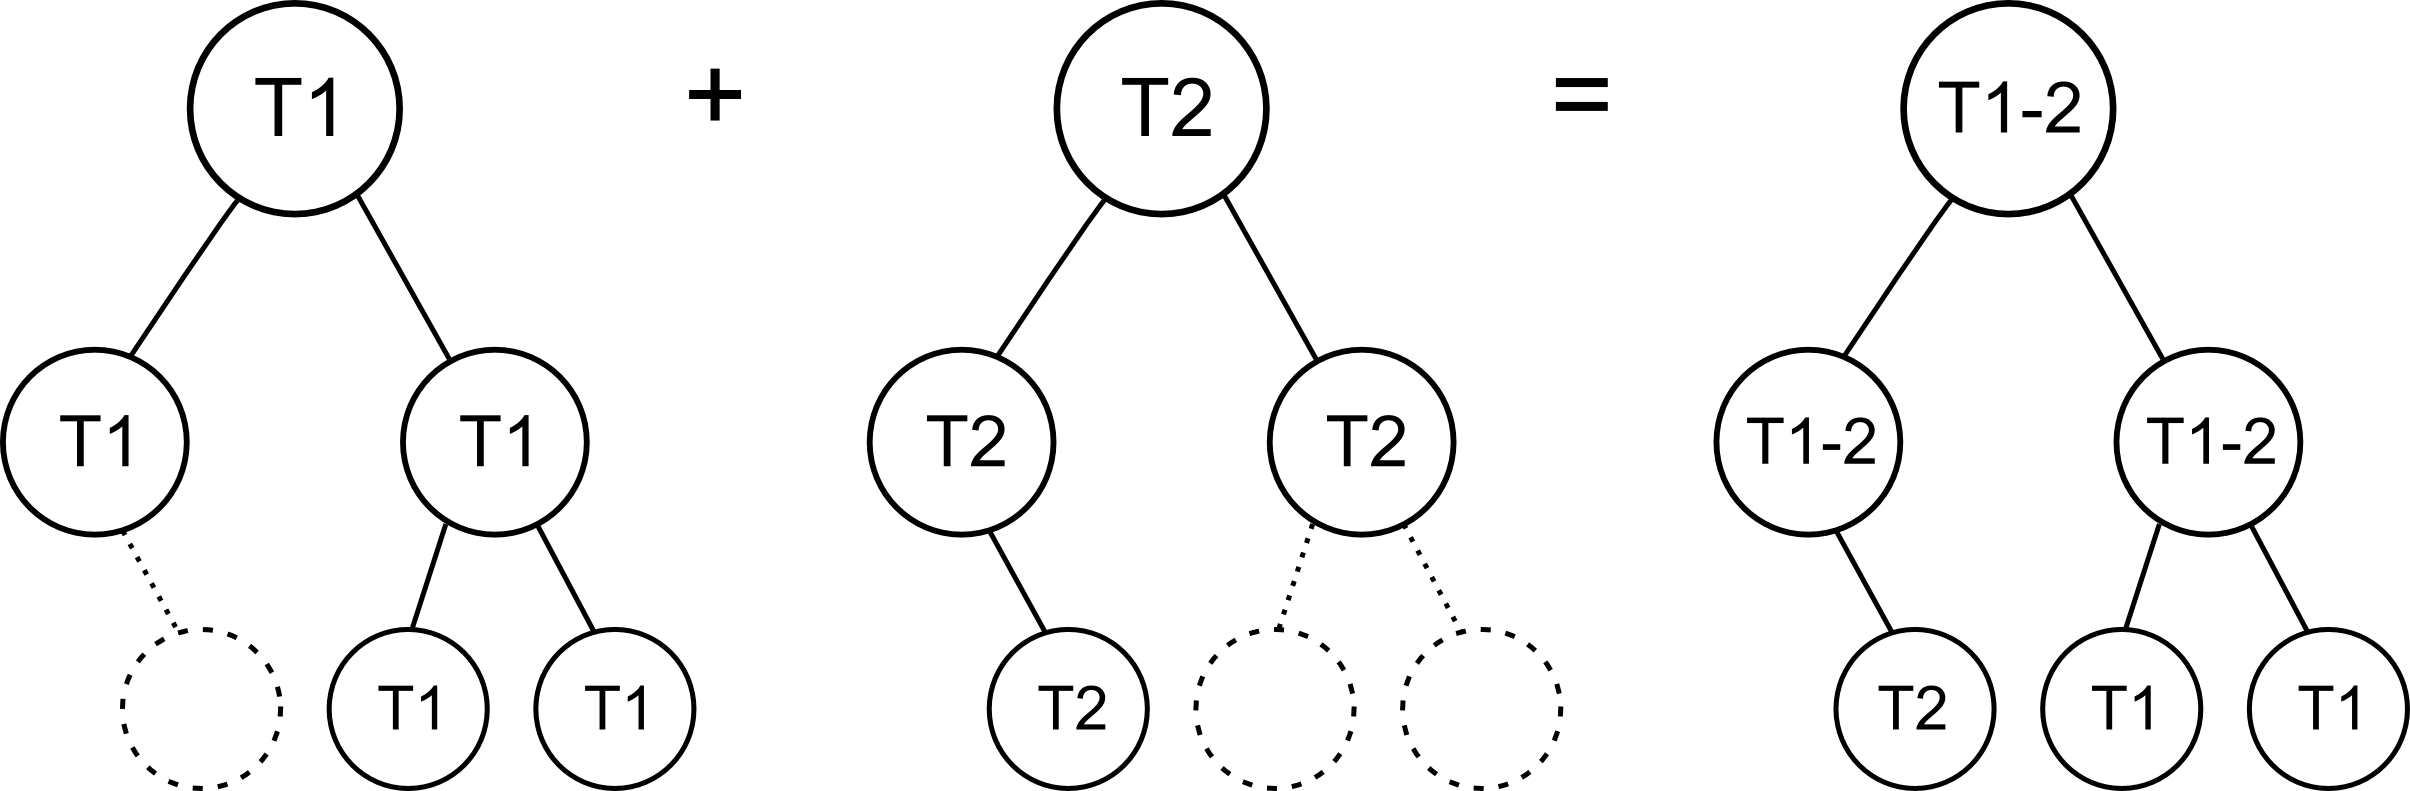
\includegraphics[width=\textwidth]{figures/chapter-approximation/figure13}
\decoRule
\caption[Illustration of unifying time steps in octree nodes]{Illustration of unifying time steps in octree nodes. For the sake of simplicity the binary tree is shown instead of octree. T1 and T2 represent approximation functions of the same data component in different time steps. Result of the union is single octree that contains sequences of corresponding time steps in its nodes.}
\label{fig:unifying-time-steps}
\end{figure}

However, not all approximation functions are preserved during merging. Each octree cell contains list of approximation functions only for key time steps, that are necessary to cover time development of discrete function in area represented by the octree cell. These key (or fixed) time steps are either specified by the user or identified automatically by the algorithm presented in Listing \ref{alg:approximation-in-time}.

Original nodal value retrieving is the same octree traversal as was depicted in Figure \ref{fig:nodal-value-computation} except for the final phase -- calculating value from approximation function in leaf octree nodes. If desired time instant is not present, then it must be interpolated from the key time steps. To find concrete time instant in the list of approximation functions the fast binary search algorithm is used.

Temporal-data-containing-octree is created by algorithm that works with already created octree having approximation functions for all time steps. At first it finds time steps that must be preserved. Those can be explicitly picked by the user or the algorithm itself determines automatically the first and the last time step as key times. Then the program traverses steps between key events of time interval. In each time step the algorithm iterates over space approximations for each loaded quantities and computes difference between each function and function created by interpolation of functions in key intervals. If this difference is lower than some preset fixed value, approximation function in current time step can be disposed because it can be created on demand in the future. Otherwise time interval is divided in current step and algorithm is recursively called on each of both intervals. It is therefore similar algorithm to approximation in space, but instead of octree a binary tree is used because there is only one temporal dimension instead of three spatial dimensions. Pseudo-code of approximation in time is shown in Listing \ref{alg:approximation-in-time}.

\begin{lstlisting}[caption=Approximation in time procedure,label=alg:approximation-in-time]
function compressTimeSteps(fromIndex, toIndex)
{
  // recursion stopping criterion
  if (toIndex - 1 <= fromIndex)
    return

  fromApproximation = timeSteps[fromIndex].Approximation
  toApproximation = timeSteps[toIndex].Approximation
  
  for (index = fromIndex + 1; index < toIndex; index++)
  {
    currentTime = timeSteps[index]
    timeFactor = (currentTime - timeSteps[fromIndex]) / (timeSteps[toIndex] - timeSteps[fromIndex])
    
    testFunction = timeSteps.Values[index].Approximation
    interpolatedFunction = InterpolatePolynomial(fromApproximation, toApproximation, timeFactor)

    sumDiffSqr = 0.0, sumFuncSqr = 0.0

    // compute difference of testFunction and interpolatedFunction
    foreach (testPoint in domainPoints)
    {
      testValue = testFunction.ComputeValue(testPoint)
      interpolatedValue = interpolatedFunction.ComputeValue(testPoint)
      diff = testValue - interpolatedValue
      
      sumDiffSqr += diff * diff
      sumFuncSqr += testValue * testValue
    }

    absoluteError = sqrt(sumDiffSqr)
    absoluteValue = sqrt(sumFuncSqr)
    relativeError = absoluteError / absoluteValue

    // if functions are not similar
    if (relativeError <= MAX_RELATIVE_ERROR)
    {
      // discard current time step
      removeTimeStep(currentTime)
    }
    else
    {
      half = (toIndex + fromIndex) / 2
      // recursive call on first half
      compressTimeSteps(fromIndex, half)
      // recursive call on second half
      compressTimeSteps(half, toIndex)
      return
    }
  }
}

// Approximation in time is called upon holes between fixed (key) time steps
// Fixed time steps are at least first and last time step and any interleaved time step specified by user
for (i = 1; i < fixedTimesIndexes.Count; i++)
{
  compressTimeSteps(fixedTimesIndexes[i - 1], fixedTimesIndexes[i])
}
\end{lstlisting}

In the case of approximation in time, we have two continuous functions that we want to compare to each other. First function is approximation function for the time step that can be potentially removed. This function is already created by spatial approximation algorithm described above. Second function is computed ad-hoc from key time steps to test if it can potentially replace the first function later. If the test succeeds (functions are similar enough) the first function can be removed entirely from octree data structure, because it can be computed from the functions in neighboring time steps.

The process of computing intermediate function from the key time steps is quite straightforward. With regard to the fact that all approximation functions have to be of the same polynomial type, each parameter of the interpolated function can be then computed as interpolation of the related parameters in two boundary functions in key time steps.

Approximation in time is made for each spatial octree node separately instead of globally for the whole mesh, because the quantity can change in time only in some parts of the mesh and in others can be constant.

%----------------------------------------------------------------------------------------
%	SUB-SUB-SECTION Difference between two functions
%----------------------------------------------------------------------------------------

\subsubsection{Difference between two functions}

The algorithm for approximation in time has to compare two continuous approximation functions to determine their similarity.

The difference $d$ of two continuous square-integrable functions $u$ and $v$ is considered as scalar value computed as

\begin{equation}
  d = \sqrt{\int_{\Omega}(u-v)^2 \diff\Omega}.
\end{equation}

If $u \neq 0$ relative difference $\hat{d}$ is then

\begin{equation}
  \hat{d} = \frac{\sqrt{\int_{\Omega}(u-v)^2\diff\Omega}}{\sqrt{\int_{\Omega}u^2\diff\Omega}}.
\end{equation}

To move from continuous to discrete world the integrals can be replaced by sums

\begin{equation}
  \int_{\Omega}f(x)\diff x = \sum_{i=1}^{m}f(x_i) w_i,
\end{equation}

where $w_i$ is the weight of the $i$-th test point with the meaning of volume surrounding the point, $x_i$ is the location of the test point and $m$ is the number of integration points. The test points in the formula are the data points situated in the area represented by approximation function $f$ in the presented algorithm.

Relative error $\tilde{d}$ is then

\begin{equation}
  \tilde{d} = \sqrt{\frac{\sum_{i=1}^{m}(u(x_i)-v(x_i))^2 w_i}{\sum_{i=1}^{m}u(x_i)^2 w_i}}.
\end{equation}

The value of $\tilde{d}$ is then compared to $\epsilon$ value. The value $\epsilon=0.001$ came from the experiments as the best-fitting value. If condition $\tilde{d} \leq \epsilon$ holds, functions $u$ and $v$ are considered equal in terms of approximation in time. The value $\epsilon$ matches \code{MAX\_RELATIVE\_ERROR} parameter in Listing \ref{alg:approximation-in-time}.

%----------------------------------------------------------------------------------------
%	SUB-SUB-SECTION Results
%----------------------------------------------------------------------------------------

\subsubsection{Results}

Results of the approximation in time are summarized in Table \ref{tab:reactor-vessel-spacetime}. For spatial approximation the trilinear regression was chosen as the method with the best results in the previous benchmark. The reactor vessel simulation results were used in the test (see Figure \ref{fig:reactor-vessel-displacements}).

\begin{table}[H]
\caption[Approximated results of reactor vessel 2D simulation (space and time)]{Reactor vessel 2D. Spatial and temporal octree approximation results.}
\label{tab:reactor-vessel-spacetime}
\centering
\begin{tabular}{| l | r | r | r |}
\hline
\tabhead{ } & \tabhead{Max error [\%]} & \tabhead{Average error [\%]} & \tabhead{Compression ratio [\%]} \\
\hline
Mean value & 100.7 \textcolor{negativeColor}{(+25.42)} & 0.7835 \textcolor{negativeColor}{(+0.16)} & 7.53 \textcolor{positiveColor}{(-47.77)}\\
Linear regression & 44.23 \textcolor{neutralColor}{(+0.0)} & 0.2262 \textcolor{negativeColor}{(+0.042)} & 2.57 \textcolor{positiveColor}{(-15.13)}\\
Trilinear regression & 81.41 \textcolor{negativeColor}{(+0.14)} & 0.2158 \textcolor{negativeColor}{(+0.041)} & 2.54 \textcolor{positiveColor}{(-14.34)}\\
\hline
\end{tabular}
\end{table}

Files with mesh topology and FEM results that were used in this benchmark can be found at \cite{XXX-15}. Time compression procedure presented in Listing \ref{alg:approximation-in-time} was applied to already created octree-based structure containing approximations of original data values. Generation of this octree is described in section \ref{sec:approximation-in-space}.
\chapter{SVD used for compression of FEA results}
\label{chapter:SVD}

Singular Value Decomposition (SVD) is a well known factorization method that provides rich information about matrix systems \cite{Baker2005, Kalman1996, Golub1996, Duintjer2012}. One of its many applications is image compression where it can significantly reduce size of data representing image while preserving quality of image appearance. Considering the fact that the results from FEM analyses can be viewed as a series of arbitrary rectangular matrices, the implementation of compression algorithm based on SVD is straightforward as it can be applied to any rectangular matrix. This chapter contains the description of the compression method based on SVD that is the key part of the storage format presented in this thesis. The content of this chapter is also published in \cite{Benes2018}.

%----------------------------------------------------------------------------------------
%	SECTION Mathematical background
%----------------------------------------------------------------------------------------

\section{Mathematical background}

Singular value decomposition is based on a theorem from linear algebra which says that a rectangular matrix $\mtrx{A} \in \mathbb{R}^{m \times n}$ can be decomposed into the product of three matrices - an orthogonal matrix $\mtrx{U} \in \mathbb{R}^{m \times m}$, a diagonal
matrix $\mtrx{S} \in \mathbb{R}^{m \times n}$, and the transpose of an orthogonal matrix $\mtrx{V} \in \mathbb{R}^{n \times n}$:

\begin{equation}
\mtrx{A} = \mtrx{U} \mtrx{S} \mtrx{V}^\mathsf{T},
\label{eq:svd-def}
\end{equation}

\noindent
where $\mtrx{U^\mathsf{T}U} = \mtrx{I}$, $\mtrx{V^\mathsf{T}V} = \mtrx{I}$. The columns of $\mtrx{U}$ are orthonormal eigenvectors of $\mtrx{AA^\mathsf{T}}$, which are called the left singular vectors. The columns of $\mtrx{V}$ are orthonormal eigenvectors of $\mtrx{A^\mathsf{T}A}$ called the right singular vectors. $\mtrx{S}$ (sometimes referred to as $\mtrx{\Sigma}$) is a diagonal matrix containing singular values in descending order, which are at the same time the nonzero square roots of the eigenvalues of $\mtrx{AA^\mathsf{T}}$ and $\mtrx{A^\mathsf{T}A}$.

SVD can be seen as a method for transforming correlated variables into a set of uncorrelated ones. At the same time, SVD is a method for ordering the dimensions based on variation and identifying the dimension with the largest variation. Once this dimension is identified, it is possible to find the best approximation of the original data points using fewer dimensions. Hence, SVD can be seen as a method for data reduction/compression.

\subsection{SVD compression}

This is the basic idea behind SVD: taking a high dimensional, highly variable set of data points and reducing it to a lower dimensional space that exposes the substructure of the original data more clearly and orders it from the largest variation to the least. What makes SVD practical for data compression applications is that variation below a particular threshold can be simply ignored to massively reduce data with assurance that the main relationships of interest have been preserved.

The objective of a compression algorithm is to reduce amount of data representing FEM results and also the ability to reconstruct original data from its smaller representation. This saves storage capacity and also accelerates the data transfer between computers as the analysis itself and the post-processing of results is sometimes done on different workstations.

A compression method can be lossy or lossless. Lossless methods are able to fully reconstruct original data. Lossy methods, on the other hand, produce only approximations of original data.

SVD is used in this thesis as a part of the compression algorithm. The SVD method applied to arbitrary matrix produces decomposition that consists of corresponding singular values and singular vectors. This process is fully reversible (with the assumption that the numerical errors are negligible). The original matrix can be reconstructed by the multiplication of decomposed parts. However, the compression algorithm is based on modification of decomposition to create low-rank approximation matrix. The reconstructed matrix slightly differs from the original matrix and algorithm therefore performs lossy compression.

\subsection{Low-rank approximation matrix}

From the definition of SVD in (\ref{eq:svd-def}) and from the properties of SVD, the fact follows that a matrix can be represented in the form of its SVD components as a sum of $k$ rank-1 matrices

\begin{equation}
\mtrx{A}=\sum_{i=1}^{k} s_{i}\mathbf{u}_{i}\mathbf{v}_{i}^{\mathsf{T}},
\label{eq:svd-expansion}
\end{equation}

\noindent
where $s_i$ is the $i$-th singular value of matrix $\mtrx{A}$, $\mathbf{u}_i$ and $\mathbf{v}_i$ are corresponding singular vectors of matrix $\mtrx{A}$, and $k = \mathrm{min}(m, n)$. Considering the fact that singular values are ordered $s_{1} \geq s_{2} \geq s_{3} \geq ... \geq s_{k}$, the above formula implies that the first term of the sum would have the highest contribution and the last term would have the lowest contribution to matrix~$\mtrx{A}$. Therefore, if we take only first $r$ members of the above summation we get an approximation matrix

\begin{equation}
\mtrx{A'}=\sum_{i=1}^{r} s_{i}\mathbf{u}_{i}\mathbf{v}_{i}^{\mathsf{T}}.
\label{eq:svd-approx-expansion}
\end{equation}

Quality of approximation depends on the magnitude of the singular values omitted from the approximation formula, namely $s_{r+1} ...  s_{k}$. The compression algorithm is based on an assumption that the first singular value is order-of-magnitude higher than singular values at the end of the decomposition sequence. In special cases, when $r=k$, or $s_{i}=0$ for all $i > r$, the omitted singular values do not contribute to the sum and the compression is therefore lossless. In other cases, approximation error has to be calculated and taken into account to avoid loss of important details in data.

The main goal of the compression algorithm is to find a compromise between low approximation error and high compression ratio $c$ which is calculated using the formula

\begin{equation}
c=\frac{r(m+n+1)}{m n},
\label{eq:cr-def}
\end{equation}

\noindent
where $m$ is the number of rows and $n$ is the number of columns of matrix $\mtrx{A}$. Explanation of the compression ratio formula is best done using Figure~\ref{fig:lowrank_svd}. Light color represents the part of matrix decomposition that is to be stored in the output file as a low-rank approximation of the input.

\begin{figure}[H]
\centering
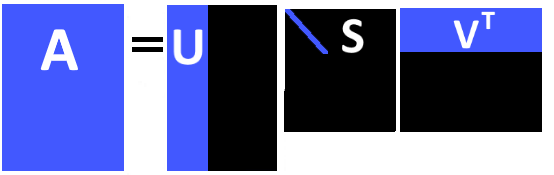
\includegraphics[width=0.7\textwidth]{figures/chapter-SVD/low_rank_decomposition_diagram}
\decoRule
\caption[Singular value decomposition illustration.]{Decomposition of input matrix $\mtrx{A}$ into diagonal matrix of singular values $\mtrx{S}$ and matrices of left and right singular vectors. Light color illustrates low-rank approximation.}
\label{fig:lowrank_svd}
\end{figure}

\subsection{Error estimation}
\label{sec:error-estimation}

Low-rank approximation matrix method, which was described above, is a lossy compression technique. Several error metrics are used to control the quality of results.

\begin{itemize}

\item \textbf{Mean Square Error}
\begin{equation}
\mathit{MSE}=\frac{1}{m n} \sum_{i=1}^{m} \sum_{j=1}^{n} (a_{ij} - a'_{ij})^{2},
\label{eq:mse-def}
\end{equation}

\noindent
where $a_{ij}$ represents an element of the original matrix and $a'_{ij}$ represents an element of the
reconstructed matrix of dimension $m \times n$.

\item \textbf{Rooted Mean Square Deviation}
\begin{equation}
\mathit{RMSD} = \sqrt{\mathit{MSE}}.
\label{eq:rmsd-def}
\end{equation}

\item \textbf{Normalized Rooted Mean Square Deviation}
\begin{equation}
\mathit{NRMSD} = \frac{\mathit{RMSD}}{X_{max}-X_{min}}=\frac{\sqrt{\mathit{MSE}}}{X_{max}-X_{min}},
\label{eq:nrmsd-def}
\end{equation}

\noindent
where $X_{min}$ and $X_{max}$ are elements of input matrix $\mtrx{A}$ with minimum and maximum value, respectively. This error metric is able to measure and compare errors in datasets with different scales. Therefore, it is the main parameter that is used to control the quality of compression in the proposed compression algorithm.

\item \textbf{Peak Signal to Noise Ratio}

$\mathit{PSNR}$ is most commonly used to measure the quality of reconstruction of lossy compression methods (e.g. image compression). The signal in this case is the original data, and the noise is the error introduced by compression. $\mathit{PSNR}$ is an approximation to human perception of reconstruction quality. This metric is not so important in area of FEM analyses, where the human perception of visualizations is not as important as the exact mathematical accuracy of approximations. The reason to include $\mathit{PSNR}$ in results is in particular to allow comparison with other image-related compression methods. $\mathit{PSNR}$ is usually expressed in terms of the logarithmic decibel scale (dB)

\begin{eqnarray}
\mathit{PSNR} &=& 10\log_{10}\frac{(X_{max}-X_{min})^{2}}{\mathit{MSE}} =
\\
&=& 20\log_{10}\frac{X_{max}-X_{min}}{\sqrt{\mathit{MSE}}}=20\log_{10}\frac{1}{\mathit{NRMSD}} = \nonumber
\\
&=& -20\log_{10}\mathit{NRMSD}. \nonumber
\label{eq:psnr-def}
\end{eqnarray}

\item \textbf{Normalized Maximum Error}
\begin{equation}
\mathit{NME} = \frac{\lVert \mtrx{A} - \mtrx{A'} \lVert_{\max}}{X_{max}-X_{min}} = \frac{\max\limits_{ij}(a_{ij} - a'_{ij})}{X_{max}-X_{min}}.
\label{eq:nme-def}
\end{equation}

\end{itemize}

\subsection{Randomized SVD}

There are many algorithms with different approaches to compute singular value decompositions. One approach is based on diagonalization of the matrix which essentially yields the whole decomposition at the same time. The other approach is the use of an iterative algorithm that yields one or several singular values at a time and can be stopped after desired number of singular values and vectors has been computed. Although these algorithms have proven to work very well for relatively small matrices, they are not well suited for using with large data sets. The exact SVD of a $m \times n$ matrix has computational complexity $\mathrm{O}(\mathrm{min}(mn^2, m^2n))$ using the ``big-O'' notation. When applied on large data sets it tends to be very time-consuming. Also, the modern hardware architectures use caches to optimize reading of consecutive memory blocks. As these algorithms often need random access to the memory where the input matrix is stored, it can increase communication between different levels in memory hierarchy, which causes higher latency when accessing data. From a numerical linear algebra perspective, an additional problem resulting from increasing matrix sizes is that noise in the data, and propagation of rounding errors, become increasingly problematic.

In \cite{Candes2011, Woolfe2008, Martinsson2011, Szlam2014}, there are described randomized methods for constructing approximate matrix factorizations which offer significant speedups over classical methods. The particular implementation of the randomized decomposition is based on the algorithm described in \cite{Halko2011}. The authors proposed an algorithm for efficient computation of low-rank approximation to a given matrix. The method uses random sampling to identify a subspace that captures most of the action of a matrix. The input matrix is compressed to this subspace, and deterministic manipulations are then used to obtain the desired low-rank factorization. For a matrix that is too large to fit in fast memory, the randomized techniques require only a constant number of passes over the data, as opposed to $\mathrm{O}(k)$ passes for classical algorithms.

The algorithm can be split into two main computational stages. The first stage is to construct a low-dimensional subspace that captures the action of the matrix. To be more formal, this stage is to compute an approximate basis for the range of the input matrix $\mtrx{A}$. This basis matrix $\mtrx{Q}$ is required to have orthonormal columns and

\begin{equation}
\mtrx{A} \approx \mtrx{Q} \mtrx{Q}^{\mathsf{T}} \mtrx{A}.
\end{equation}

\noindent
Matrix $\mtrx{Q}$ is desired to contain as few columns as possible while producing accurate approximation of matrix $\mtrx{A}$ at the same time.

The second stage is to use $\mtrx{Q}$ to obtain approximate SVD factorization of $\mtrx{A}$. This can be achieved using simple deterministic steps:

\begin{enumerate}
\item Construct $\mtrx{B} = \mtrx{Q}^{\mathsf{T}} \mtrx{A}$.
\item Compute an exact SVD of the small matrix: $\mtrx{B}=\mtrx{W}\mtrx{\widetilde{S}}\mtrx{\widetilde{V}}^{\mathsf{T}}$.
\item Set $\mtrx{\widetilde{U}}=\mtrx{Q}\mtrx{W}$.
\end{enumerate}

The main challenge is therefore to efficiently construct $r$ orthonormal vectors forming the matrix $\mtrx{Q}$ that (nearly) span the range of $\mtrx{A}$; $r$ is the desired rank of approximation and is supposed to be substantially less then both dimensions of $\mtrx{A}$. After that an SVD that closely approximates $\mtrx{A}$ can be constructed (closely in the sense that the spectral norm of the difference between $\mtrx{A}$ and the approximation to $\mtrx{A}$ is small relative to the spectral norm of $\mtrx{A}$).

In order to estimate the range of matrix $\mtrx{A}$, it is applied to a collection of $r$ random vectors. The result of applying $\mtrx{A}$ to any vector is a vector in the range of $\mtrx{A}$, and if the matrix is applied to $r$ random vectors, the results will nearly span the range of $\mtrx{A}$ with extremely high probability. Mathematical proofs given in \cite{Halko2011} and \cite{Witten2015} show that the probability of missing a substantial part of the range of $\mtrx{A}$ is negligible if the vectors to which we apply $\mtrx{A}$ are sufficiently random (i.e. entries of these vectors are independent and identically distributed).

Therefore, the matrix $\mtrx{A}$ is applied to a random Gaussian matrix $\mtrx{\Omega}$ that contains $r$ columns with random normally distributed entries yielding the matrix $\mtrx{Y} = \mtrx{A} \mtrx{\Omega}$. Applying the Gram-Schmidt process (or any other method for constructing QR decomposition) produces the decomposition $\mtrx{Y}=\mtrx{Q}\mtrx{R}$, where columns of $\mtrx{Q}$ are an orthonormal basis for the range of $\mtrx{Y}$, and since columns of $\mtrx{Y}$ nearly span the range of $\mtrx{A}$, $\mtrx{Q}$ is an orthonormal basis for the approximate range of $\mtrx{A}$.

$\mtrx{A}$ is then decomposed as
\begin{equation}
\mtrx{A} \approx \mtrx{Q}\mtrx{Q}^{\mathsf{T}}\mtrx{A} = \mtrx{Q}\mtrx{B} = \mtrx{Q}\mtrx{W}\mtrx{\widetilde{S}}\mtrx{\widetilde{V}}^{\mathsf{T}} = \mtrx{\widetilde{U}}\mtrx{\widetilde{S}}\mtrx{\widetilde{V}}^{\mathsf{T}}.
\end{equation}

\noindent
The algorithm produces matrices $\mtrx{\widetilde{U}}$ and $\mtrx{\widetilde{V}}$ with orthonormal columns being approximations of the left and the right singular vectors of matrix $\mtrx{A}$, and a nonnegative diagonal matrix $\mtrx{\widetilde{S}}$ that contains approximations of the first $r$ singular values of matrix $\mtrx{A}$. For a dense input matrix, randomized SVD algorithm requires $\mathrm{O}(mn \log{r})$ floating-point operations, substantially less than classical algorithms.


%----------------------------------------------------------------------------------------
%	SECTION Implementation
%----------------------------------------------------------------------------------------

\section{Implementation}

% SVD is applied on matrices. The first thing to do is therefore to assemble an input matrix. ...
% As an example, temperature field, vector of nodal displacements, strain tensor evaluated in integration points, etc. can serve. There are two similar sets of results. One is generated by a non-linear algorithms, where several incremental steps are stored and the other is generated by time integration, where results in particular time steps are stored. ...

Results from the finite element method are scalar, vector or tensor fields represented by discrete values calculated in nodes of the mesh or in integration points on finite elements. In order to compress data, an auxiliary matrix~$\mtrx{A}$ has to be assembled from the results. The number of rows of the matrix~$\mtrx{A}$ is equal to the number of incremental or time steps while the number of columns is equal to the number of points in which the results are stored. Such auxiliary matrix is assembled for each scalar field and for each component of the vector and tensor fields. It means, three matrices corresponding to the displacement in the $x$, $y$, and $z$ directions are assembled for the vector of displacements in three-dimensional problems.

There are two main reasons to store particular results in separate matrices. First, the size of matrices is smaller than the size of a matrix which contains all results and therefore SVD will be performed faster. Second, the magnitudes of particular fields are very different (the stress tensor components are several order of magnitude larger than the components of the displacement vector) and the data compression algorithm would suppress the fields with small magnitudes. Once the matrix $\mtrx{A}$ is assembled for each field, the compression algorithm can be applied on it. It is purely algebraic procedure and no information about geometry of the mesh is needed.

Let us assume that the matrix is not empty and is full rank. Then it follows from the formula (\ref{eq:cr-def}) that if $r$ is equal to the rank of matrix $\mtrx{A}$, the compression ratio is always higher than one. In other words the memory consumption of stored decomposition is bigger than the size of the original matrix. To make the compression algorithm applicable, the parameter $r$ must satisfy the condition

\begin{equation}
r<\frac{m n}{m+n+1}.
\label{eq:r-ineq}
\end{equation}

\noindent
Considering the usual shape of matrix containing FEM results, this inequality is easily satisfiable even for the $r$ being close to the rank of the original matrix as in the typical case the number of nodes or integration points is much higher than the number of analysis steps and therefore $m \ll n$.

\subsection{Algorithm description}
Once SVD is calculated, the compression algorithm removes a certain number of singular values and corresponding singular vectors. The remaining singular values and vectors represent the compressed data. There are two strategies that influence the way how to preserve the number of singular values -- resulting size and quality. Each strategy is assigned a control parameter that determines compression ratio or approximation error.

\paragraph{Compression ratio}
If the focus is only on the size of compressed data, the rank $r$ of the approximation matrix can be calculated by the formula

\begin{equation}
r=\ceil*{c \times \frac{m n}{m+n+1}},
\label{eq:rank-from-comp-ratio}
\end{equation}

\noindent
where $c$ is the compression ratio, $0 \leq c \leq 1$ ($0$ results in absolute compression while $1$ results in no compression); $\ceil*{.}$ is the ceiling function.

\paragraph{Approximation error}
In a usual case, the most important measure to take into account is the approximation error. Algorithm is trying to minimize the compression ratio while at the same time ensuring that predefined approximation error threshold is not exceeded. To quantify the error, the Normalized root-mean-square deviation ($\mathit{NRMSD}$) is used. The normalized error metric enables working with various data sets that have different scales. $\mathit{NRMSD}$ is defined in Section \ref{sec:error-estimation}.

To effectively calculate the final rank of the approximation matrix from the desired approximation error, the interesting property of singular values

\begin{equation}
\sum_{i=1}^{m} \sum_{j=1}^{n} (a_{ij})^{2} = \sum_{i=1}^{k}{s_{i}^{2}},
\label{eq:elem-sqr-sigma-sqr}
\end{equation}

\noindent
where $k=\mathrm{min}(m, n)$, i.e. the smallest of two dimensions of the matrix $\mtrx{A}$, is made use of. The above formula states that the sum of squared elements of the matrix $\mtrx{A}$ equals to the sum of squared singular values $s_{i}$ of the same matrix $\mtrx{A}$.

Using formulas \eqref{eq:svd-expansion} and \eqref{eq:svd-approx-expansion} the equation \eqref{eq:elem-sqr-sigma-sqr} can be applied to the difference between original matrix $\mtrx{A}$ and approximation matrix $\mtrx{A'}$

\begin{equation}
\sum_{i=1}^{m} \sum_{j=1}^{n} (a_{ij} - a'_{ij})^{2} = \sum_{i=r+1}^{k}{s_{i}^{2}},
\end{equation}

\noindent
where the term on the right-hand side is the sum of squares of those singular values of the matrix $\mtrx{A}$ that are going to be cut away by the compression algorithm. The equation can be rewritten using the definition of $\mathit{MSE}$ in \eqref{eq:mse-def} to

\begin{equation}
\mathit{MSE} \times m n = \sum_{i=r+1}^{k} s_{i}^{2}
\end{equation}

\noindent
and using \eqref{eq:nrmsd-def} further to

\begin{equation}
(\mathit{NRMSD} \times (X_{max}-X_{min}))^{2} \times m n = \sum_{i=r+1}^{k} s_{i}^{2}.
\end{equation}

Then $\mathit{NRMSD}$ can be used as a quality metric for the compression algorithm because normalization makes it usable for different datasets. Calculation of rank of the approximation matrix is depicted as pseudo-code in Algorithm \ref{alg:rank-calculation}. Algorithm uses the inequality

\begin{equation}
e > \frac{\sqrt[]{\frac{\sum_{i=r+1}^{k} s_{i}^{2}}{m n}}}{X_{max}-X_{min}}
\end{equation}

\noindent
to test whether the desired rank has been reached; $e$ is $\mathit{NRMSD}$ used as an error threshold that can not be exceeded to achieve desired quality of approximation.

\begin{algorithm}
  \caption{Calculation of rank for approximation matrix from maximum allowed error.}\label{rankAlgorithm}
  \label{alg:rank-calculation}
  \begin{algorithmic}[1]
  	\INPUT maximum allowed error ($e: e > 0$), array with singular values ($S: S.length > 0$), element count ($c: c > 0$), maximum element value ($x_{max}$), minimum element value ($x_{min}: x_{max} > x_{min}$)
    \OUTPUT rank of resulting matrix
    \Procedure{CalculateRank}{$e, S, c, x_{max}, x_{min}$}
      \State $\mathit{MSE} \gets 0$
      \State $\mathit{NRMSD} \gets 0$
      \State $rank \gets S.length$
      \While{$\mathit{NRMSD} < e$}\Comment{repeat until max error is reached}
        \State $\mathit{MSE} \gets \mathit{MSE} + S[rank]/c$ \Comment{calculate $\mathit{MSE}$ for current rank}
        \State $\mathit{NRMSD} \gets \sqrt{\mathit{MSE}} / (x_{max} - x_{min})$ \Comment{normalize error}
        \State $rank \gets rank - 1$ \Comment{decrement rank for next loop}
      \EndWhile
      \State \textbf{return} $rank + 1$ \Comment{Add one to not exceed maximum allowed error}
    \EndProcedure
  \end{algorithmic}
\end{algorithm}

\subsection{Optimization}

Computational complexity of the exact SVD algorithm is $\mathrm{O}(m^2n)$, where $m<n$. This theoretical algorithm complexity is confirmed by two benchmarks where the dependency of the execution time on the varying matrix dimension is shown. The results of the benchmarks are depicted in Figure \ref{fig:ExeTime_rows} and Figure \ref{fig:ExeTime_columns}. Several observations were made from the results:

\begin{itemize}
\item The algorithm is most efficient in cases where one dimension of the input matrix is very small compared to the other. However, this is almost always the case when compressing results from FEM -- number of incremental or time steps seldom exceeds hundreds.
\item Moreover, incremental or time steps can be devided into smaller ranges and the algorithm can be applied on each range separately. This will improve performance and can also increase quality of compression if the key time steps on the range boundaries are carefully selected.
\item The randomized SVD algorithm has the same order of algorithmic complexity when full decomposition is required, but yet can significantly reduce execution time. However, the benchmarks are not designed to highlight the benefits of randomized SVD algorithms. The main advantage of the randomized SVD is in the ability to choose the rank of the approximation matrix in advance. In that case only limited number of singular values and corresponding singular vectors are calculated and algorithm performs much faster.
\end{itemize}

Storage size of SVD itself can also be optimized. $\mtrx{S}$, being a diagonal matrix, can be stored as single list of singular values $s_{i}$, or can be even multiplied with the matrix of left singular vectors $\mtrx{U}$.


%----------------------------------------------------------------------------------------
%	SECTION Results
%----------------------------------------------------------------------------------------

\section{Results}

All procedures presented here were tested on a common PC having Intel Core i5-4690K @ 3.5GHz CPU with 16GB RAM, running on Microsoft Windows 10 64-bit operating system.

The first benchmark was designed to measure computational complexity of the SVD algorithm. Series of 100 random matrices with standard distribution were generated and execution times were recorded and averaged. The execution time with respect to the number of the stored incremental or time steps (the number of rows in the matrix $\mtrx{A}$) is depicted in Figure \ref{fig:ExeTime_rows} while the execution time with respect to the number of points, where the results are stored (the number of columns of the matrix $\mtrx{A}$), is depicted in Figure \ref{fig:ExeTime_columns}. Especially in Figure \ref{fig:ExeTime_columns}, it is clearly visible that the randomized SVD algorithm is much faster than the classical one.

These results confirm that the SVD implementation has computational complexity $\mathrm{O}(m^2n)$, where $m$ is number of rows, $n$ is number of columns, and $m < n$. In case of $m > n$ the complexity would be $\mathrm{O}(mn^2)$ as the algorithm takes advantage of non-squareness in that its complexity is quadratic only in the smaller dimension.

\begin{figure}[H]
\centering
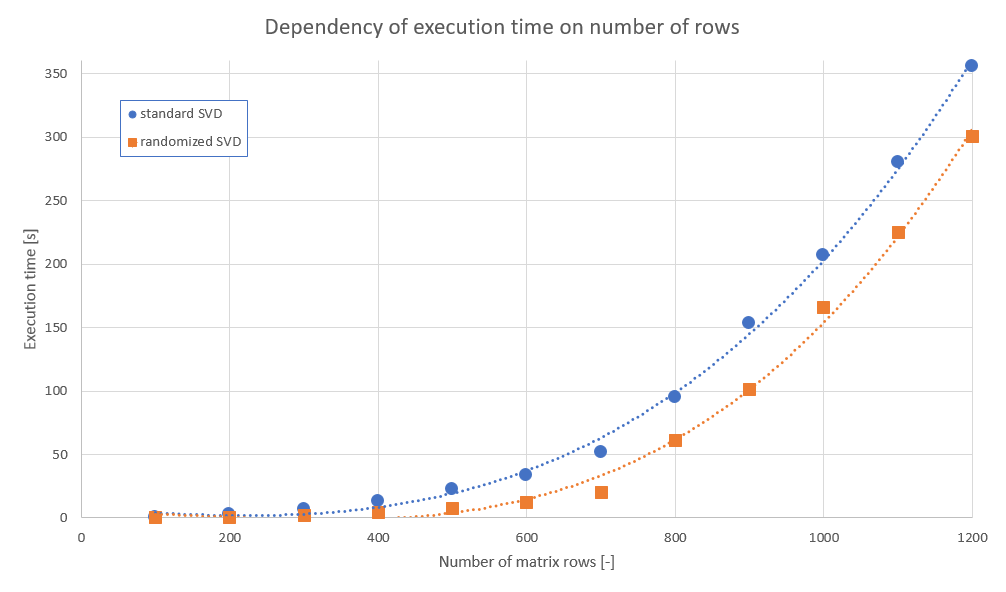
\includegraphics[width=\textwidth]{figures/chapter-SVD/executionTime_varyingRows}
\decoRule
\caption[Dependency of SVD execution time on number of rows.]{Dependency of SVD execution time on $m$ (having fixed $n = 10000$ and $r=min(m,n)$).}
\label{fig:ExeTime_rows}
\end{figure}

\begin{figure}[H]
\centering
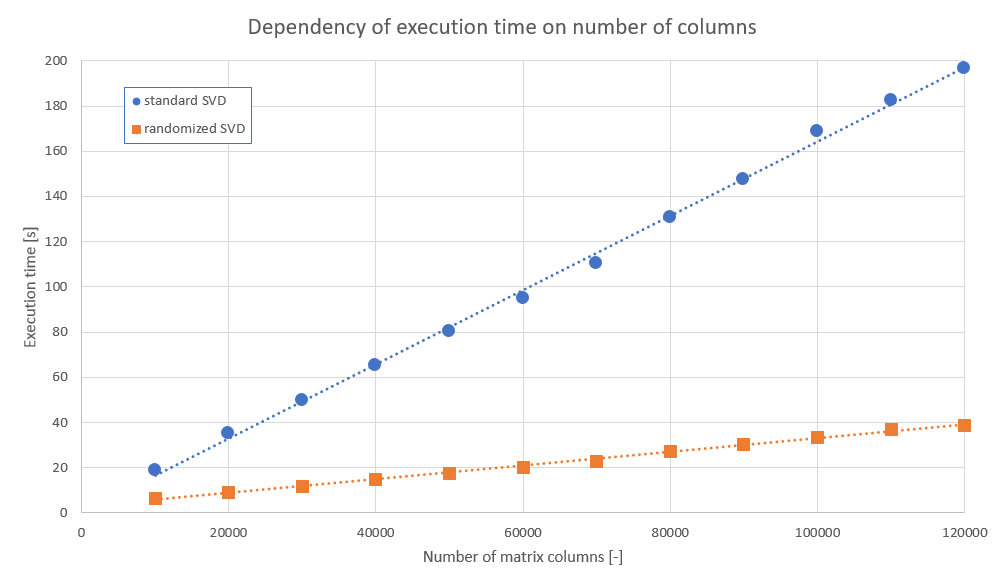
\includegraphics[width=\textwidth]{figures/chapter-SVD/executionTime_varyingColumns}
\decoRule
\caption[Dependency of SVD execution time on number of columns.]{Dependency of SVD execution time on $n$ (having fixed $m = 100$ and $r=min(m,n)$).}
\label{fig:ExeTime_columns}
\end{figure}

% reactor containment
Behavior of the compression strategy introduced is presented on three real world examples. First example is an analysis of aging of nuclear power plant's containment made from prestressed concrete. Finite element mesh used in this analysis is in Figure \ref{fig:temelin:mesh}. More details about the analysis can be found in \cite{Kruis2012} and \cite{Koudelka2009}. This analysis includes high number of analysis time steps (thousands) with very little differences between them. There is therefore potential for compression to be very effective (compression ratio to be very low) as proven in Figure \ref{fig:temelin:NRMSD} that examines the impact of changes in the compression ratio to the mean error of approximation.

\begin{figure}[H]
\centering
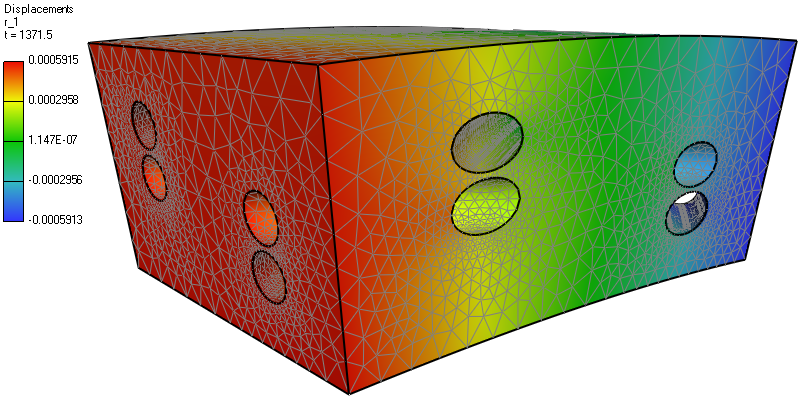
\includegraphics[width=\textwidth]{figures/chapter-SVD/temelin_screenshot}
\decoRule
\caption[Results visualization: reactor containment 3D.]{Segment of reactor containment analyzed. Results visualization (displacement field, x component).}
\label{fig:temelin:mesh}
\end{figure}

\begin{figure}[H]
\centering
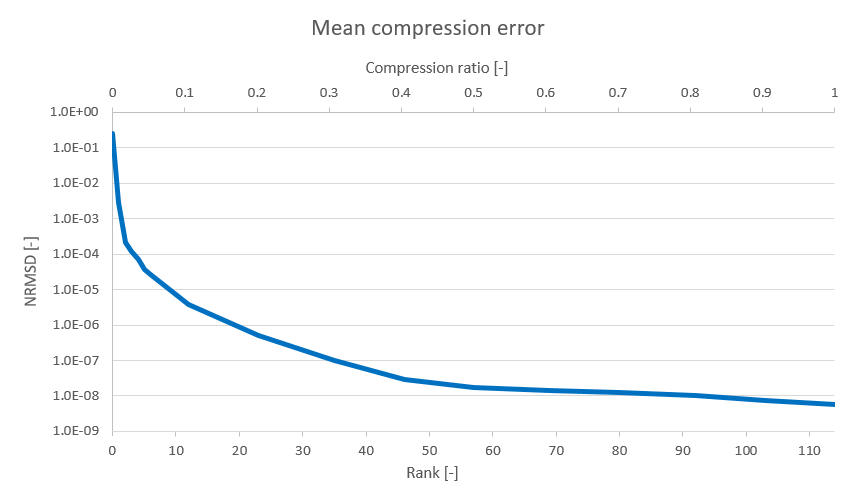
\includegraphics[width=\textwidth]{figures/chapter-SVD/temelin_NRMSD}
\decoRule
\caption[Dependence of NRMSD on compression ratio and rank (reactor containment 3D).]{Dependence of $\mathit{NRMSD}$ on $c$ and $r$ for reactor containment analysis results.} % ...$c$ (and $r$)...
\label{fig:temelin:NRMSD}
\end{figure}

% geological layers
Figure \ref{fig:chotkova:mesh} shows results from an analysis of geological layers which was based on theory of plasticity. More details can be found in \cite{Koudelka2006}. This project was chosen mainly to study behavior of compression algorithm when dealing with high discontinuities in data in spatial dimension (as can be seen in visualization). As summarized in Figure \ref{fig:chotkova:NRMSD} and Figure \ref{fig:chotkova:MaxError} this has negligible effect ($\mathit{NRMSD}$ and $\mathit{NME}$ are bellow 1\% even for very small $r$ -- 3 out of 22) on quality of compression.

\begin{figure}[H]
\centering
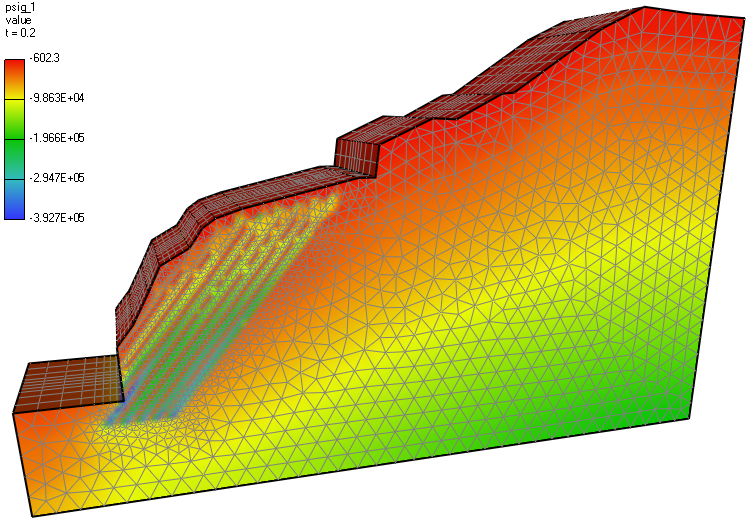
\includegraphics[width=\textwidth]{figures/chapter-SVD/chotkova_screenshot}
\decoRule
\caption[Results visualization: geological layers.]{Analysis of geological layers. Results visualization (stress field, sigma XX component).}
\label{fig:chotkova:mesh}
\end{figure}

\begin{figure}[H]
\centering
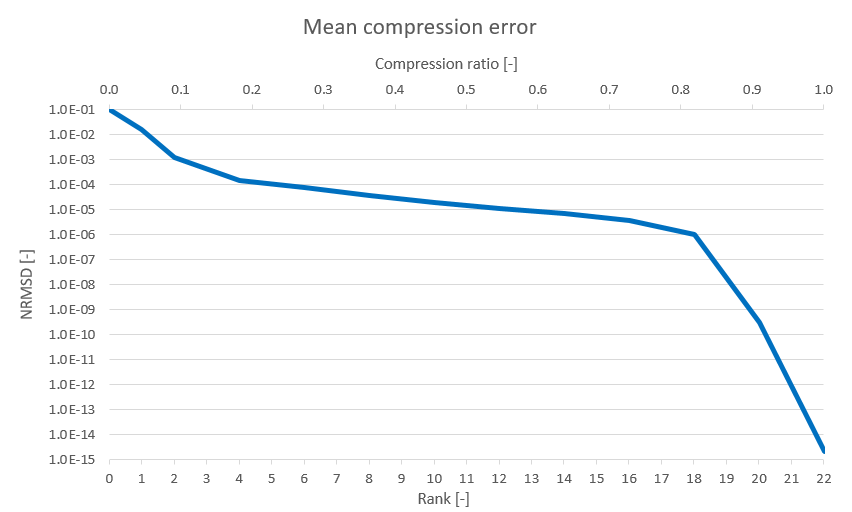
\includegraphics[width=\textwidth]{figures/chapter-SVD/chotkova_NRMSD}
\decoRule
\caption[Dependence of NRMSD on compression ratio and rank (geological layers).]{Dependence of $\mathit{NRMSD}$ on $c$ and $r$ for results of geological layers project.}
\label{fig:chotkova:NRMSD}
\end{figure}

\begin{figure}[H]
\centering
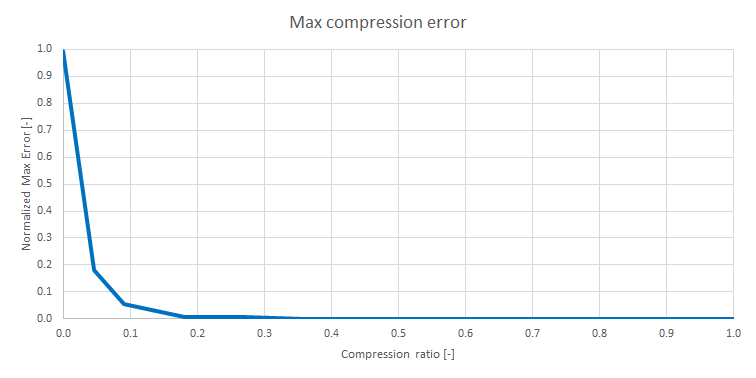
\includegraphics[width=\textwidth]{figures/chapter-SVD/chotkova_MaxError}
\decoRule
\caption[Dependence of NME on compression ratio and rank (geological layers).]{Dependence of $\mathit{NME}$ on $c$ and $r$ for results of geological layers project.}
\label{fig:chotkova:MaxError}
\end{figure}

% reactor vessel 2D
Figure \ref{fig:mechaxisym:mesh} contains visualization of results of two-dimensional analysis, where axisymmetric description was used for analysis of aging of a reactor vessel. Details about the analysis can be found in \cite{Kruis2005}. There are exactly 232 analysis time steps. The resulting data has linear function character with several discontinuities in temporal dimension. There are few time steps in which resulting discrete functions have very different values compared to neighboring time steps. This was supposed to have negative impact on the quality of compression. However, as can be seen in Figure \ref{fig:mechaxisym:NRMSD}, the quality is better than expected; e.g., if the rank of approximation matrix is set to 3 (compared to 232 being the rank of the original matrix) the normalized relative error ($\mathit{NRMSD}$) does not exceed $10^{-5}$.

\begin{figure}[H]
\centering
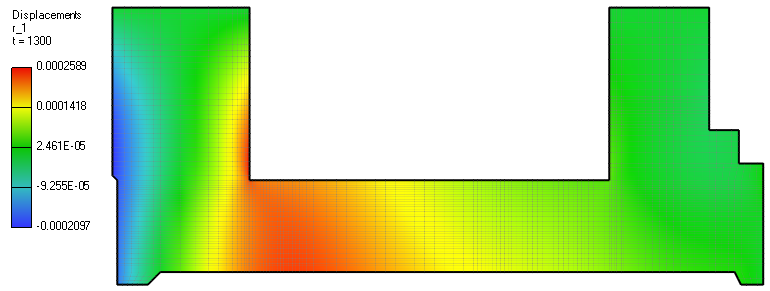
\includegraphics[width=\textwidth]{figures/chapter-SVD/mechaxisym_screenshot}
\decoRule
\caption[Results visualization: reactor vessel 2D.]{2D model of a reactor vessel. Results visualization (displacement field, x component).}
\label{fig:mechaxisym:mesh}
\end{figure}

\begin{figure}[H]
\centering
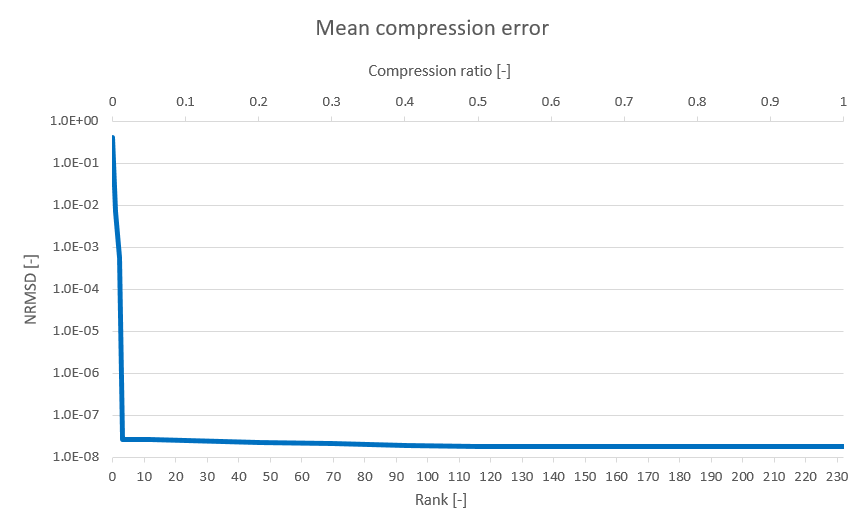
\includegraphics[width=\textwidth]{figures/chapter-SVD/mechaxisym_NRMSD}
\decoRule
\caption[Dependence of NRMSD on compression ratio and rank (reactor vessel 2D).]{Dependence of $\mathit{NRMSD}$ on $c$ and $r$ for reactor vessel analysis results.}
\label{fig:mechaxisym:NRMSD}
\end{figure}

% PSNR
Figure \ref{fig:PSNR} summarizes the compression error for all three benchmarks using $\mathit{PSNR}$ metric. $\mathit{PSNR}$ is defined using logarithm (see Equation (\ref{eq:psnr-def}) for definition), and is included here mainly as a comparison to other image-related compression methods whose quality is often expressed by $\mathit{PSNR}$. Figure \ref{fig:PSNR_rand} contains the same information for the randomized SVD algorithm.

\begin{figure}[H]
\centering
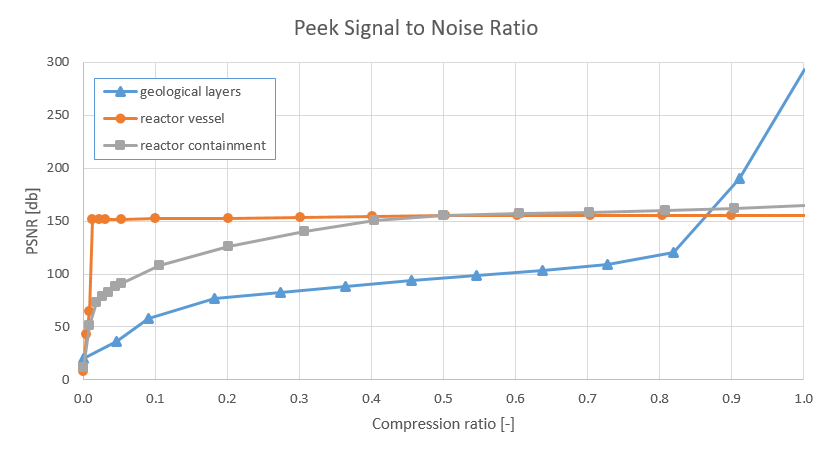
\includegraphics[width=\textwidth]{figures/chapter-SVD/PSNR}
\decoRule
\caption[Dependence of PSNR on compression ratio and rank.]{Dependence of $\mathit{PSNR}$ value on $c$ and $r$ calculated for different SVD decompositions.}
\label{fig:PSNR}
\end{figure}

\begin{figure}[H]
\centering
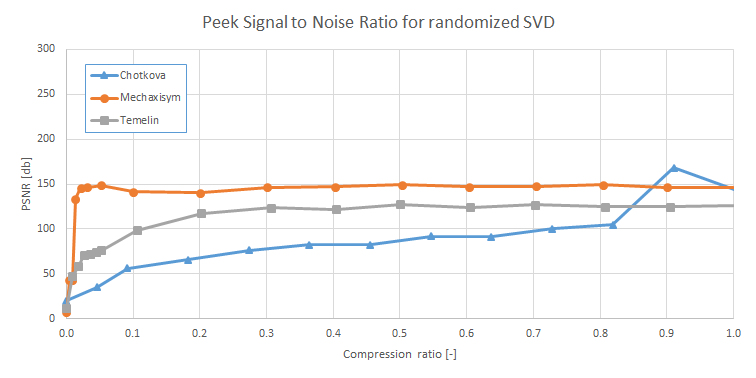
\includegraphics[width=\textwidth]{figures/chapter-SVD/PSNR_rand}
\decoRule
\caption[Dependence of PSNR on compression ratio and rank (randomized SVD).]{Dependence of $\mathit{PSNR}$ value on $c$ and $r$ calculated for different randomized SVD decompositions.}
\label{fig:PSNR_rand}
\end{figure}

% Execution times
Besides the error also the execution speed of compression algorithm was measured. In Figure \ref{fig:temelin:ExeTime}, there is a comparison of execution times for standard versus randomized SVD compression algorithms. Interestingly, execution time of standard SVD is independent of target rank whereas execution time of randomized SVD decreases linearly with decreasing target rank. If the rank is known ahead, the fact can be taken advantage of.

\begin{figure}[H]
\centering
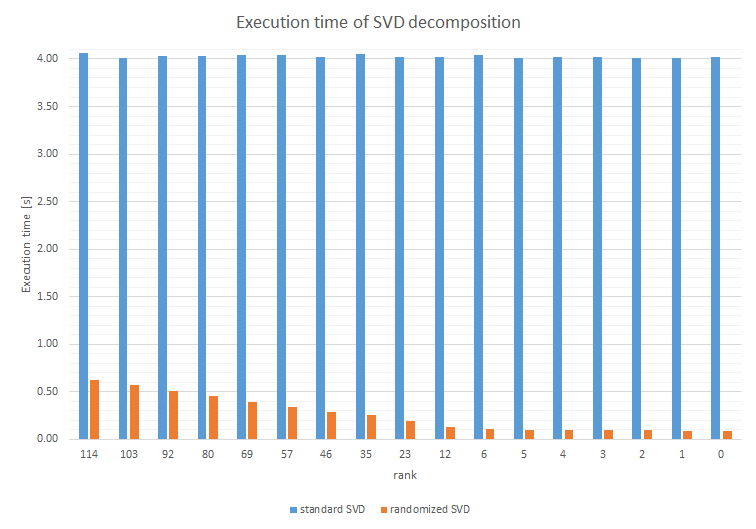
\includegraphics[width=\textwidth]{figures/chapter-SVD/temelin_ExecutionTime}
\decoRule
\caption[Execution time of standard and randomized SVD decompositions.]{Variation of execution time of standard and randomized SVD decompositions calculated for reactor containment analysis results.}
\label{fig:temelin:ExeTime}
\end{figure}

The memory consumption of compressed results for reactor containment analysis is summarized in Table \ref{tab:mem-consum}. For different values of compression ratio it shows memory size in megabytes. In this benchmark, the compression ratio $c$ is an input parameter to the compression algorithm. As follows from the Equation (\ref{eq:rank-from-comp-ratio}), the value of the compression ratio directly affects the amount of singular values ought to be removed from SVD. Size factor describes the final outcome of compression when compared to the original size.

\begin{table}[H]
\caption{Memory consumption of compressed results. 3D reactor containment analysis.}
\label{tab:mem-consum}
\centering
\begin{tabular}{| r | r | r |}
\hline
\tabhead{compression ratio (\textit{\textbf{c}})} & \tabhead{memory consumption [MB]} & \tabhead{size factor} \\
\hline
1.00 & 2002.1 & 1 \\
0.50 & 1006.9 & 0.5002 \\
0.10& 211.9 & 0.1053 \\
0.01 & 35.3 & 0.0176 \\
\hline
\end{tabular}
\end{table}

\chapter{Conclusions}
\label{chapter:conclusions}

\todo{TODO: Final remarks \ldots}\\
% Vsechny cile splneny!
\todo{Vyjmenovat cile z kapitoly Aims a ke kazdemu napsat, jak se povedlo splneni. Dolozit to vysledkami z kapitoly Overlall results.}\\
\todo{Zopakovat proc jsem vlastne delal co jsem delal. Proc jsem vynalezal novy format. Proc jsem resil kompresi dat.}\\
\todo{Shrnuti, co se povedlo, co se nepovedlo (nedostatky jednotlivych metod reseni - aproximace nevhodna napr pro diskontinuity, SVD super).}\\
\todo{Porovnani s jinymi resenimi predstavenymi v kapitole related work. Kompresi meshe (napr. PM, LoD) jsem vlastne uplne odmitnul - nevyplati se, je vypocetne narocne, soustredim se pouze na kompresi vysledku}\\
\todo{Future work? moznosti pro vylepseni SVD komprese: main features for optimization: key time steps (time step span compression), Randomized SVD, Parallelization, Sparse matrix of details, prenasobeni U matice singularnimi cisly, trochu usetrim pamet, mohu pouzit vzorkovani...}\\


%----------------------------------------------------------------------------------------
%	THESIS CONTENT - APPENDICES
%----------------------------------------------------------------------------------------

\appendix % Cue to tell LaTeX that the following "chapters" are Appendices

\chapter{Data format for storage and transport of FEM results}
\label{appendix:data-format}

% Examples of solution.json, summary.json, mesh.json, attribute.json, and result.json files

Listing \ref{lst:solution.json} ...

\begin{lstlisting}[style=json,caption=Example of solution.json document,label=lst:solution.json]
{
    "Id": 42,
    "ProjectName": "Shear beam 3D",
    "Location": "https://fea-cloud-service.net/postprocess/42",
    "Results": [
      {
        "MeshRecordNames": [
          "beam.msh"
        ],
        "DataRecordNames": [
          "beam.res"
        ]
      }
    ],
    "Layers": [
      {
        "Id": "5b585758-9f64-4790-a765-64709951931a",
        "Name": "master",
        "FilterType": null,
        "Children": [
          {
            "Id": "09dfdc8c-a75b-48e1-b319-a9624312a5a5",
            "Name": "deformation (scale: 0.6)",
            "FilterType": "Deformation",
            "Children": [
              {
                "Id": "ee52969e-f862-4daf-85b9-5a8224197669",
                "Name": "slice (offset: -0.1569261)",
                "FilterType": "Slice"
              },
              {
                "Id": "a86486b1-53eb-43cc-aa22-d670bcdea163",
                "Name": "slice (offset: -0.4757478)",
                "FilterType": "Slice"
              },
              {
                "Id": "6c6c4b8a-2280-4b4b-a51f-fcd5149f1d94",
                "Name": "slice (offset: -0.8751443)",
                "FilterType": "Slice"
              }
            ]
          },
          {
            "Id": "96ca950c-0767-4439-b57a-35384ea351a7",
            "Name": "isosurface DISPLACEMENTS/X(1) = -0.0001",
            "FilterType": "IsoSurface"
          },
          {
            "Id": "2a3c47be-2f06-48f5-adfd-30777aea092c",
            "Name": "isosurface DISPLACEMENTS/X(1) = -0.0003",
            "FilterType": "IsoSurface"
          },
          {
            "Id": "7e5f043b-9900-427e-8d38-839ff1b8e27c",
            "Name": "isosurface DISPLACEMENTS/X(1) = -0.0007",
            "FilterType": "IsoSurface"
          }
        ]
      }
    ]
}
\end{lstlisting}

Listing \ref{lst:summary.json} ...

\begin{lstlisting}[style=json,caption=Example of summary.json document,label=lst:summary.json]
{
    "Id": "5b585758-9f64-4790-a765-64709951931a",
    "Name": "master",
    "ParentId": null,
    "Filter": null,
    "Meshes": [
      {
        "Index": 1,
        "TimeSteps": [1.0, 2.0, 3.0, 4.0, 5.0, 6.0],
        "Attributes": [
          {
            "Index": 1,
            "FieldName": "ElementProperty",
            "Location": "Cells"
          }
        ]
      }
    ],
    "Fields": {
      "CRACK_WIDTH": { ... } ,
      "DISPLACEMENTS": {
        "Components": {
          "X(1)": {
            "TimeSteps": {
              "1": { "MeshIndex": 1, "DataIndex": 4 },
              "2": { "MeshIndex": 1, "DataIndex": 4 },
              "3": { "MeshIndex": 1, "DataIndex": 4 },
              "4": { "MeshIndex": 1, "DataIndex": 4 },
              "5": { "MeshIndex": 1, "DataIndex": 4 },
              "6": { "MeshIndex": 1, "DataIndex": 4 }
            }
          },
          "X(2)": {
            "TimeSteps": {
              "1": { "MeshIndex": 1, "DataIndex": 5 },
              "2": { "MeshIndex": 1, "DataIndex": 5 },
              "3": { "MeshIndex": 1, "DataIndex": 5 },
              "4": { "MeshIndex": 1, "DataIndex": 5 },
              "5": { "MeshIndex": 1, "DataIndex": 5 },
              "6": { "MeshIndex": 1, "DataIndex": 5 }
            }
          },
          "X(3)": {
            "TimeSteps": {
              "1": { "MeshIndex": 1, "DataIndex": 6 },
              "2": { "MeshIndex": 1, "DataIndex": 6 },
              "3": { "MeshIndex": 1, "DataIndex": 6 },
              "4": { "MeshIndex": 1, "DataIndex": 6 },
              "5": { "MeshIndex": 1, "DataIndex": 6 },
              "6": { "MeshIndex": 1, "DataIndex": 6 }
            }
          }
        }
      },
      "EXTERNAL_FORCES": { ... },
      "STRAIN": { ... },
      "STRESS": { ... }
    }
}
\end{lstlisting}

Listing \ref{lst:mesh.json} ...

\begin{lstlisting}[style=json,caption=Example of mesh.json document,label=lst:mesh.json]
{
    "LayerId": "5b585758-9f64-4790-a765-64709951931a",
    "Index": 1,
    "NumberOfPoints": 434,
    "NumberOfCells": 324,
    "NumberOfEdges": 0,
    "Center": [0.6375, 0.095, 0.16],
    "Radius": 0.6719607,
    "PointCoordinates": "//9/MwAAADIK16M+//9/MwAAADJvEoM+gDSjPQAAADIK16M+//9/M1yPwj0K16M+gDSjPQAAAD...",
    "CellTypes": "DAwMDAwMDAwMDAwMDAwMDAwMDAwMDAwMDAwMDAwMDAwMDAwMDAwMDAwMDAwMDAwMDAwMDAwMDAwMDAwMD..."
}
\end{lstlisting}

Listing \ref{lst:attribute.json} ...

\begin{lstlisting}[style=json,caption=Example of attribute.json document,label=lst:attribute.json]
{
    "LayerId": "5b585758-9f64-4790-a765-64709951931a",
    "Index": 1,
    "MeshIndex": 1,
    "FieldName": "ElementProperty",
    "Location": "Cells",
    "Compression": null,
    "Encoding": {
      "DataType": "Int32",
      "OriginalLength": 324,
      "Offset": 160,
      "Length": 164,
      "DefaultValue": "18"
    },
    "Data": "EwAAABMAAAATAAAAEwAAABMAAAATAAAAEwAAABMAAAATAAAAEwAAABMAAAATAAAAEwAAABMAAAATAAAAEwAAAB..."
}
\end{lstlisting}

Listing \ref{lst:result.json} ...

\begin{lstlisting}[style=json,caption=Example of result.json document,label=lst:result.json]
{
    "LayerId": "5b585758-9f64-4790-a765-64709951931a",
    "Index": 4,
    "MeshIndex": 1,
    "FieldName": "DISPLACEMENTS",
    "ComponentName": "X(1)",
    "TimeSteps": [1.0, 2.0, 3.0, 4.0, 5.0, 6.0],
    "Location": "Points",
    "Compression": {
      "Method": "SVD",
      "Rows": 6,
      "Columns": 434,
      "Rank": 3
    },
    "Encoding": {
      "DataType": "Float64",
      "OriginalLength": 2640,
      "Offset": 0,
      "Length": 2640
    },
    "Data": "47HYqWHLML9OLoc9P8tAv5nfIqKPa1S/BoMRvASgbL+E47yyIMJ5v47IymmBdYK/ZcAwsn55IL+uuEUHN3swv1..."
}
\end{lstlisting}

%----------------------------------------------------------------------------------------
%	BIBLIOGRAPHY
%----------------------------------------------------------------------------------------

%\nocite{*} % check for unused references (package refcheck); comment out to filter out unused references

\printbibliography[heading=bibintoc]

%----------------------------------------------------------------------------------------

\end{document}
